\documentclass[12pt,a4paper,oneside]{book} % twoside for draf

\usepackage[utf8]{inputenc}
\usepackage[T5]{fontenc}
\usepackage{tgtermes}

\usepackage{amsmath}
\usepackage{amssymb}
\usepackage{fancyhdr}

\usepackage{titlesec}
\usepackage{titletoc}
\usepackage{listings}
\usepackage[bookmarks=true]{hyperref}
\usepackage[left=3cm,right=2cm,top=2.5cm,bottom=3cm]{geometry}
\usepackage{graphicx}
\usepackage{hyperref}
\usepackage{tikz}
\usepackage{varwidth}
\usepackage{float}
\usepackage{color}
\usepackage{multirow}
\usepackage{booktabs}
\usepackage[linesnumbered,lined,ruled,resetcount,algochapter,procnumbered]{algorithm2e}
\usepackage{svg}
\usepackage{tabularx}
\usepackage{nomencl}
\usepackage{scrfontsizes}
\usepackage{longtable}
\usepackage{multicol}
% \usepackage[toc,page]{appendix}
\usepackage{tocbibind}
\usepackage{adjustbox}
\usepackage[numbers]{natbib}
\usepackage{makecell}
\usepackage{longtable}
\usepackage{multirow}
% \usepackage{algpseudocode}
\usepackage{settings/uetthesis}
\usepackage[toc]{appendix}
\usepackage{bm}
\usepackage{dirtytalk}
\usepackage{slashbox}
\usepackage{subcaption}
\usepackage{glossaries}
\setcitestyle{square}

\counterwithin{figure}{chapter}
\usepackage{xpatch}
\usepackage{setspace}

\makeatletter
% \input{numeric.bbx}
\makeatother

\setlength{\parskip}{6pt}

\usetikzlibrary{calc}

\setlength{\parindent}{10mm}
\renewcommand{\baselinestretch}{1.31}
\graphicspath{{images/}}
\renewcommand{\listalgorithmcfname}{Danh sách thuật toán}
\renewcommand{\algorithmcfname}{Thuật toán}
\renewcommand{\nomname}{Danh sách ký hiệu, viết tắt}
\renewcommand\appendixtocname{Phụ lục}

\newenvironment{procalgorithm}[1][htb]
  {\renewcommand{\algorithmcfname}{Thủ tục}% Update algorithm name
   \begin{algorithm}[#1]
  }{\end{algorithm}}

\newtheorem{definition}{Định nghĩa}
\SetKwRepeat{Do}{do}{while}%

\titlecontents{chapter}%
[0pt]%
{\vspace{1ex}}%
{\bfseries Chương \thecontentslabel\quad}%
{\bfseries}%
{\bfseries\hfill\contentspage}


\let\chapappname\chaptername


\definecolor{dkgreen}{rgb}{0,0.6,0}
\definecolor{gray}{rgb}{0.5,0.5,0.5}
\definecolor{mauve}{rgb}{0.58,0,0.82}




\renewcommand{\lstlistingname}{Source}
\renewcommand\thechapter{\arabic{chapter}}
\renewcommand\thesection{\thechapter.\arabic{section}}
\renewcommand\thesubsection{\thesection.\arabic{subsection}}
% \renewcommand\thesubsubsection{\thesection.\thesubsection.\arabic{subsubsection}}
\renewcommand{\thetable}{\thechapter.\arabic{table}}
\renewcommand{\thefigure}{\thechapter.\arabic{figure}}
\renewcommand{\thealgocf}{\thechapter.\arabic{algocf}}
\renewcommand{\thedefinition}{\thechapter.\arabic{definition}}

\begin{document}



%======================================================
\titleclass{\subsubsubsection}{straight}[\subsection]

\newcounter{subsubsubsection}[subsubsection]
\renewcommand\thesubsubsubsection{\thesubsubsection.\arabic{subsubsubsection}}
\renewcommand\theparagraph{\thesubsubsubsection.\arabic{paragraph}} % optional; useful if paragraphs are to be numbered

\titleformat{\subsubsubsection}
{\normalfont\normalsize\bfseries}{\thesubsubsubsection}{1em}{}
\titlespacing*{\subsubsubsection}
{0pt}{3.25ex plus 1ex minus .2ex}{1.5ex plus .2ex}

\makeatletter
\renewcommand\paragraph{\@startsection{paragraph}{5}{\z@}%
	{3.25ex \@plus1ex \@minus.2ex}%
	{-1em}%
	{\normalfont\normalsize\bfseries}}
\renewcommand\subparagraph{\@startsection{subparagraph}{6}{\parindent}%
	{3.25ex \@plus1ex \@minus .2ex}%
	{-1em}%
	{\normalfont\normalsize\bfseries}}
\def\toclevel@subsubsubsection{4}
\def\toclevel@paragraph{5}
\def\toclevel@paragraph{6}
\def\l@subsubsubsection{\@dottedtocline{4}{7em}{4em}}
\def\l@paragraph{\@dottedtocline{5}{10em}{5em}}
\def\l@subparagraph{\@dottedtocline{6}{14em}{6em}}

\setcounter{secnumdepth}{5}

\makeatother
%===============================================================



\pagestyle{plain}
\frontmatter

% ----------------------TRANG BÌA----------------------
%-------TITLE PAGE 1------%
\begin{titlepage}
	\center
	\begin{tikzpicture}[overlay,remember picture]
		\draw [line width=3pt,rounded corners=0pt,]
		($ (current page.north west) + (25mm,-25mm) $)
		rectangle
		($ (current page.south east) + (-15mm,25mm) $);
		\draw [line width=1pt,rounded corners=0pt]
		($ (current page.north west) + (26.5mm,-26.5mm) $)
		rectangle
		($ (current page.south east) + (-16.5mm,26.5mm) $);
	\end{tikzpicture}
	
	{\bfseries ĐẠI HỌC QUỐC GIA HÀ NỘI\\ TRƯỜNG ĐẠI HỌC CÔNG NGHỆ}\\[1cm]
	
\includegraphics[width=0.25\linewidth]{uet_logo.png}\\[1cm]
	{\Large  \bfseries Phan Tiến Đạt}\\[1.5cm]
	
	{ \LARGE \bfseries ARGOS: ORCHESTRATING GRAPH REASONING WITH ADAPTIVE AGENTS FOR ROBUST CONVERSATIONAL RECOMMENDATION }\\[0.05cm]
    
	\hfill\\[2cm]
	{\large \bfseries KHÓA LUẬN TỐT NGHIỆP ĐẠI HỌC HỆ CHÍNH QUY }\\	
	\vspace{4mm}
	{\large \bfseries Ngành: Hệ thống Thông tin}	
	\hfill\\[4.3cm]	
	{\bfseries HÀ NỘI - 2026}\\	
	\vfill
\end{titlepage}
%-------TITLE PAGE 2------%
\begin{titlepage}
	\center
	\begin{tikzpicture}[overlay,remember picture]
	\draw [line width=3pt,rounded corners=0pt,]
	($ (current page.north west) + (25mm,-25mm) $)
	rectangle
	($ (current page.south east) + (-15mm,25mm) $);
	\draw [line width=1pt,rounded corners=0pt]
	($ (current page.north west) + (26.5mm,-26.5mm) $)
	rectangle
	($ (current page.south east) + (-16.5mm,26.5mm) $);
	\end{tikzpicture}
	
	{\bfseries ĐẠI HỌC QUỐC GIA HÀ NỘI\\ TRƯỜNG ĐẠI HỌC CÔNG NGHỆ}\\[2cm]
	
	{\Large  \bfseries Phan Tiến Đạt}\\[2cm]
		{ \LARGE \bfseries ARGOS: ORCHESTRATING GRAPH REASONING WITH ADAPTIVE AGENTS FOR ROBUST CONVERSATIONAL RECOMMENDATION }\\[0.05cm]
	\hfill\\[1.5cm]
	{\large \bfseries KHÓA LUẬN TỐT NGHIỆP ĐẠI HỌC HỆ CHÍNH QUY }\\	
	\vspace{4mm}
	{\large \bfseries Ngành: Hệ thống Thông tin}
	\hfill\\[2.cm]
	\begin{flushleft}
	    	{\large \bfseries Cán bộ hướng dẫn: TS. Nguyễn Thị Hậu}
	\end{flushleft}
        \hfill\\[0.6cm]
        % \begin{flushleft}
	    % {\large \bfseries Cán bộ đồng hướng dẫn: }
	% \end{flushleft}

        \vspace{3.0cm}
        \vfill	  
	{\bfseries HÀ NỘI - 2026}\\		
	\vfill		
\end{titlepage}
%-------TITLE PAGE 3 (English)------%
\begin{titlepage}
	\center
	\begin{tikzpicture}[overlay,remember picture]
	\draw [line width=3pt,rounded corners=0pt,]
	($ (current page.north west) + (25mm,-25mm) $)
	rectangle
	($ (current page.south east) + (-15mm,25mm) $);
	\draw [line width=1pt,rounded corners=0pt]
	($ (current page.north west) + (26.5mm,-26.5mm) $)
	rectangle
	($ (current page.south east) + (-16.5mm,26.5mm) $);
	\end{tikzpicture}
	
	{\bfseries VIETNAM NATIONAL UNIVERSITY, HANOI\\ UNIVERSITY OF ENGINEERING AND TECHNOLOGY}\\[2cm]
	
	{\Large \bfseries Phan Tien Dat}\\[2cm]
	\begin{spacing}{1.8}
		{\LARGE \bfseries
		ARGOS: ORCHESTRATING GRAPH REASONING WITH ADAPTIVE AGENTS FOR ROBUST CONVERSATIONAL RECOMMENDATION}
	\end{spacing}
	\hfill\\[1.5cm]
	% {\large \bfseries GRADUATION THESIS}\\	
	% \vspace{4mm}
	{\Large \bfseries Major: Information System}
	\hfill\\[3cm]
	\begin{flushleft}
		{\large \bfseries Supervisor: Dr. Nguyen Thi Hau}
	\end{flushleft}
	\hfill\\[1.2cm]
	% \begin{flushleft}
	% 	{\large \bfseries Co-Supervisor: }
	% \end{flushleft}

	\hfill\\[2.4cm]	
	{\bfseries HANOI - 2026}\\		
	\vfill		
\end{titlepage}

% ----------------------LỜI CẢM ƠN----------------------
\chapter*{Lời cảm ơn}
\addcontentsline{toc}{chapter}{Lời cảm ơn}

Trước hết, tôi xin bày tỏ lòng biết ơn sâu sắc đến TS. Nguyễn Thị Hậu vì sự hỗ trợ kiên định, sự dìu dắt vô giá và những định hướng khoa học sâu sắc trong suốt quá trình tôi thực hiện khóa luận này. Sự tận tâm và chuyên môn của cô không chỉ là kim chỉ nam giúp tôi hoàn thiện công trình nghiên cứu, mà còn đóng vai trò nền tảng trong sự phát triển tư duy cá nhân của tôi. Nếu không có sự động viên không ngừng và sự dẫn dắt chu đáo của cô, nghiên cứu này đã không thể trở thành hiện thực.

Bên cạnh đó, tôi xin được bày tỏ lòng biết ơn sâu sắc đến toàn thể các thầy cô tại Trường Đại học Công nghệ - Đại học Quốc gia Hà Nội. Trong suốt 4 năm học tập tại trường, tôi đã được nuôi dưỡng trong một môi trường giáo dục chuyên nghiệp, đầy cảm hứng và nhân văn. Sự tận tâm trong giảng dạy cùng những khối kiến thức mà các thầy cô truyền đạt đã giúp tôi xây dựng một nền tảng tri thức vững chắc.

Cuối cùng, tôi xin trân trọng cảm ơn gia đình và tất cả những người thân yêu đã luôn đồng hành, là chỗ dựa tinh thần vững chắc và tạo mọi điều kiện tốt nhất để tôi có thể hoàn thành khóa luận tốt nghiệp này.

% ----------------------CAM ĐOAN----------------------
\chapter*{Lời cam đoan}
\addcontentsline{toc}{chapter}{Lời cam đoan}

Tôi xin cam đoan rằng luận văn này là kết quả nghiên cứu của chính bản thân tôi, được thực hiện dưới sự hướng dẫn khoa học của các thầy cô. Toàn bộ nội dung, số liệu, kết quả và các phân tích trong luận văn đều do tôi trực tiếp thực hiện, hoặc được tham khảo từ những nguồn tài liệu khoa học đáng tin cậy và đã được trích dẫn, ghi rõ nguồn theo đúng quy định.  

Tôi khẳng định rằng luận văn này không sao chép của bất kỳ công trình nào khác, không vi phạm bản quyền của cá nhân hay tổ chức nào. Mọi ý tưởng, phương pháp, hay tài liệu sử dụng từ các công trình nghiên cứu của người khác đều đã được tôi trích dẫn và ghi nhận đầy đủ.  

Tôi cam kết rằng tất cả những tuyên bố trên đều là sự thật. Tôi xin hoàn toàn chịu trách nhiệm trước pháp luật cũng như các quy định của Trường Đại học Công nghệ - Đại học Quốc gia Hà Nội về những cam đoan trên.
\\

\begin{flushright}
	\begin{varwidth}{\linewidth}\centering
		Hà Nội, ngày \ldots\space tháng \ldots\space năm 2026\\
		\bigbreak
		Sinh viên\\[1.5cm]
		Phan Tiến Đạt
	\end{varwidth}
\end{flushright}


% ----------------------MỤC LỤC----------------------
\renewcommand{\contentsname}{Mục lục}
\tableofcontents

% ----------------------- Abstract -----------------
\chapter*{Tóm tắt}
\addcontentsline{toc}{chapter}{Tóm tắt}
\changefontsizes[16pt]{13pt}

Hệ thống gợi ý hội thoại (Conversational Recommender System - CRS) đóng vai trò trung tâm trong việc giải quyết bài toán thông tin cá nhân hóa thông qua tương tác ngôn ngữ tự nhiên. Tuy nhiên, sự kết hợp giữa các Mô hình ngôn ngữ lớn (LLM) và các kho tri thức cấu trúc vẫn tồn tại những rào cản về tính xác thực của dữ liệu và năng lực suy luận linh hoạt trong các kịch bản thực tế.

Khóa luận này đề xuất hệ thống \textbf{ARGOS} (Adaptive Reasoning and Graph Orchestration System), một khung làm việc đa tác tử được kế thừa và phát triển từ mô hình tiền đề \textbf{GRACE} (công trình nghiên cứu của chính tác giả đã được công bố tại hội nghị quốc tế SOICT 2025). Khác với các kiến trúc dòng chảy tĩnh vốn dễ gặp bế tắc khi đối mặt với các yêu cầu phức tạp, ARGOS vận hành dựa trên cơ chế cộng tác giữa các tác tử chuyên biệt: Orchestrator (Điều phối), Graph Agent (Suy luận đồ thị), Critic Agent (Kiểm định) và Relaxation Agent (Thỏa hiệp). Kiến trúc này cho phép hệ thống thực thi các vòng lặp phản hồi để tự phát hiện ảo giác, đồng thời tự động điều chỉnh chiến lược truy xuất khi gặp phải các ràng buộc mâu thuẫn từ phía người dùng.

Kết quả đánh giá thực nghiệm trên các bộ dữ liệu tiêu chuẩn ReDial và INSPIRED chứng minh rằng ARGOS không chỉ bảo toàn tính chính xác tuyệt đối nhờ sự ràng buộc vào Đồ thị tri thức, mà còn cải thiện đáng kể khả năng hiểu ý định và tính linh hoạt trong hội thoại so với kiến trúc tiền đề. Nghiên cứu này khẳng định tính hiệu quả của phương pháp tiếp cận đa tác tử trong việc xây dựng các hệ thống gợi ý hội thoại thông minh, tin cậy và có khả năng mở rộng.

\vspace{-0.5cm}
\begin{flushleft}
  \textit{\textbf{Từ khóa:} Hệ thống gợi ý hội thoại, Đồ thị tri thức, Mô hình ngôn ngữ lớn, Hệ thống đa tác tử (Multi-Agent System), GRACE, ARGOS.}

\end{flushleft}



\thispagestyle{empty}

\renewcommand{\listfigurename}{Danh sách hình vẽ}
\listoffigures

\renewcommand{\listtablename}{Danh sách bảng}
\listoftables

% ----------------------CHÚ THÍCH VIẾT TẮT----------------------
\chapter*{Thuật ngữ}
\addcontentsline{toc}{chapter}{Thuật ngữ}
\begin{table}[h!]

\resizebox{\textwidth}{!}{
\begin{tabular}{|c|c|p{0.5\textwidth}|}
\hline
\multicolumn{1}{|c|}{\textbf{Từ viết tắt}} & \multicolumn{1}{c|}{\textbf{Thuật ngữ}}                                                 & \multicolumn{1}{c|}{\textbf{Ý nghĩa}}                                                                         \\ \hline
CRS & Conversational Recommender System  & Hệ thống gợi ý hội thoại \\ \hline
KG & Knowledge Graph  & Đồ thị tri thức \\ \hline
LLM & Large Language Model & Mô hình ngôn ngữ lớn \\ \hline
SLM & Small Language Model  & Mô hình ngôn ngữ kích thước nhỏ \\ \hline
RAG & Retrieval-Augmented Generation  & Sinh văn bản tăng cường truy xuất \\ \hline
ReAct & Reasoning and Acting  & Mô hình kết hợp Suy luận và Hành động \\ \hline
WRRF & Weighted Reciprocal Rank Fusion & Thuật toán hợp nhất thứ hạng có trọng số \\ \hline
SOTA & State-Of-The-Art & Các kỹ thuật/mô hình tiên tiến nhất hiện nay \\ \hline
Multi-Agent & Multi-Agent System & Hệ thống cấu thành từ nhiều tác tử độc lập \\ \hline
Recall & Recall & Độ bao phủ (Tỷ lệ tìm thấy các đối tượng phù hợp) \\ \hline
Precision & Precision & Độ chính xác (Tỷ lệ đối tượng phù hợp trong số được tìm thấy) \\ \hline
API & Application Programming Interface & Giao diện lập trình ứng dụng \\ \hline
GDBMS & Graph Database Management System & Hệ quản trị cơ sở dữ liệu đồ thị \\ \hline
\end{tabular}
}
\end{table}

\clearpage

\mainmatter
\changefontsizes[16pt]{13pt}
\pagestyle{plain}

% Đánh số 
\pagenumbering{arabic}

% ----------------------MỞ ĐẦU----------------------
\chapter*{Mở đầu}
\addcontentsline{toc}{chapter}{Mở đầu}

Sự bùng nổ của thông tin số cùng nhu cầu cá nhân hóa ngày càng cao đã thúc đẩy sự chuyển dịch mạnh mẽ từ các hệ thống gợi ý tĩnh truyền thống sang các hệ thống gợi ý hội thoại (Conversational Recommender System - CRS). Bằng cách sử dụng ngôn ngữ tự nhiên làm phương thức tương tác chủ đạo, CRS cho phép hệ thống khai thác các sở thích phức tạp, linh hoạt và xử lý các nhu cầu mơ hồ của người dùng thông qua nhiều lượt đối thoại \cite{li2018towards, christakopoulou2016towardscrs}. Các bài toán lõi của CRS bao gồm việc nắm bắt chính xác ý định người dùng từ ngữ cảnh hội thoại, sinh ra các mục gợi ý phù hợp và tạo ra phản hồi ngôn ngữ tự nhiên để tương tác. Đây là một lĩnh vực thu hút sự quan tâm lớn từ cộng đồng nghiên cứu. Việc cá nhân hóa hội thoại đóng vai trò then chốt trong việc nâng cao trải nghiệm người dùng, giữ chân khách hàng và trực tiếp thúc đẩy giá trị thương mại cho các nền tảng dịch vụ.

Tuy nhiên, việc xây dựng một hệ thống CRS hoàn thiện đưa ra những thách thức đặc biệt. Sự xuất hiện của các Mô hình ngôn ngữ lớn (LLMs) đã cách mạng hóa năng lực xử lý ngôn ngữ, nhưng việc tích hợp LLM vào CRS hiện nay vẫn vấp phải rào cản cốt lõi: Tính tin cậy của thông tin (hiện tượng ảo giác) và giới hạn về năng lực suy luận đa bước. Khác với các hệ thống phân lớp hoặc dự đoán thông thường, hệ thống gợi ý hội thoại đòi hỏi hệ thống phải liên tục đối soát ý định của người dùng với cơ sở dữ liệu thực tế (như Đồ thị tri thức) để đảm bảo không gợi ý những mục không tồn tại.

Trong các nghiên cứu trước đây, nhiều kỹ thuật và kiến trúc khác nhau đã được đề xuất nhằm giải quyết bài toán này. Các hệ thống truyền thống tăng cường tri thức như KBRD \cite{chen-etal-2019-towards}, KGSF \cite{zhou2020improvingcrs} hay KERL \cite{Qiu_2025} đã tận dụng Đồ thị tri thức nhưng lại gặp hạn chế về khả năng hiểu ngôn ngữ linh hoạt. Các phương pháp dựa trên LLM theo hướng Zero-Shot (như LLM-ReDial \cite{liang-etal-2024-llm}) tỏ ra linh hoạt nhưng rất dễ sinh ra ảo giác do phụ thuộc hoàn toàn vào trí nhớ tham số. Các phương pháp tinh chỉnh như TallRec \cite{bao2023tallrec} hay ReFICR \cite{yang-2024-reficr} mang lại độ chính xác cao nhưng tốn kém tài nguyên và thiếu linh hoạt khi cập nhật dữ liệu mới. Gần đây, việc áp dụng kỹ thuật Truy xuất tăng cường sinh (Retrieval-Augmented Generation - RAG) trên Đồ thị tri thức đã cho thấy những kết quả đầy hứa hẹn. Điển hình, kiến trúc tiền đề GRACE (Graph-Reasoning Augmented Conversational Engine) đã giải quyết hiệu quả vấn đề ảo giác thông qua luồng truy xuất lai và sử dụng mô hình ngôn ngữ nhỏ để xếp hạng lại. Tuy nhiên, GRACE và các hệ thống RAG hiện tại vẫn hoạt động theo một "đường ống tĩnh". Khi đối mặt với các kịch bản hội thoại đa tầng, nơi các ràng buộc của người dùng mâu thuẫn nhau hoặc các truy vấn không có kết quả khớp tuyệt đối, kiến trúc tĩnh bộc lộ sự hạn chế: chúng thiếu đi cơ chế tự đánh giá, tự sửa lỗi và thỏa hiệp, dẫn đến việc trả về kết quả rỗng hoặc chất lượng thấp, làm gián đoạn mạch hội thoại.

Nhìn chung, các kiến trúc tĩnh hiện tại thiếu khả năng nhận thức tình huống và không thể phân rã, đối soát các yêu cầu phức tạp một cách độc lập. Để giải quyết những hạn chế đã nêu, khóa luận được thực hiện nhằm mục đích đề xuất hệ thống \textbf{ARGOS} (Adaptive Reasoning and Graph Orchestration System) chuyển đổi từ mô hình xử lý tuyến tính sang mô hình đa tác tử. Bằng cách phân chia các chức năng vào các tác tử chuyên biệt và thiết lập vòng lặp phản hồi, khóa luận hướng tới các đóng góp chính như sau:

(1) \textbf{Chuyển đổi kiến trúc từ tĩnh sang đa tác tử thích nghi:} Khóa luận đề xuất kiến trúc cộng tác giữa các tác tử: Orchestrator, Graph Agent, Critic Agent và Relaxation Agent. Khung làm việc này loại bỏ hoàn toàn điểm nghẽn của RAG dòng chảy tĩnh bằng cách đưa vào các vòng lặp phản hồi nội bộ. Hệ thống có khả năng tự động đánh giá lại chiến lược tìm kiếm, sử dụng cơ chế dự báo trọng số động để điều phối luồng truy xuất (Semantic, Content, Graph) dựa trên phân tích hình thái ngôn ngữ của truy vấn. Khóa luận xác thực tính hiệu quả của mô hình thông qua hai bộ dữ liệu hội thoại tiêu chuẩn là ReDial và INSPIRED.

(2) \textbf{Thiết lập cơ chế kiểm định nghiêm ngặt và triệt tiêu ảo giác:} Khóa luận trình bày một phương pháp đối soát chéo độc lập thông qua tác tử \textit{Critic Agent}. Bằng cách tách rời khâu trích xuất ràng buộc cứng và khâu kiểm định, mọi ứng viên được sinh ra đều phải trải qua bộ lọc của Critic Agent đối chiếu trực tiếp với Đồ thị tri thức Neo4j. Phương pháp này loại bỏ hoàn toàn các thực thể ảo giác do LLM tự sinh, đảm bảo độ chính xác và tính minh bạch tuyệt đối cho các gợi ý.

(3) \textbf{Khả năng tự sửa lỗi và thỏa hiệp thông minh:} Khi đối diện với các yêu cầu khắt khe dẫn đến tập kết quả rỗng, \textit{Relaxation Agent} được kích hoạt. Dựa trên thuật toán phân cấp ưu tiên, hệ thống có khả năng tự động phân tích điểm nghẽn, nới lỏng các ràng buộc ít quan trọng (ví dụ: năm phát hành) và giữ lại các giá trị cốt lõi (ví dụ: phong cách đạo diễn). Khả năng tự khởi động lại luồng truy vấn với ý định đã được tái cấu trúc giúp hệ thống khôi phục hội thoại một cách tự nhiên mà không cần đến sự can thiệp thủ công từ người dùng.

(4) \textbf{Tối ưu hóa độ trễ qua cơ chế Xếp hạng hai giai đoạn:} Nhằm đảm bảo khả năng đáp ứng thời gian thực, hệ thống đề xuất tách rời quá trình xếp hạng. Việc kết hợp mô hình Reranker thương mại nhẹ gọn cho vòng lọc đầu và giới hạn sự can thiệp của LLM lớn ở vòng suy luận cuối giúp giảm thiểu đáng kể chi phí tính toán và độ trễ, trong khi vẫn duy trì được hiệu suất gợi ý vượt trội. Thông qua cơ chế này, hệ thống thiết lập mốc hiệu năng SOTA mới so với các mô hình tinh chỉnh hàng đầu.

Phần còn lại của khóa luận được tổ chức như sau:

Chương 1 giới thiệu tổng quan, đặt vấn đề, tổng hợp các nghiên cứu liên quan, xác định khoảng trống nghiên cứu cùng mục tiêu và đóng góp của khóa luận. Chi tiết các kiến thức nền tảng về Hệ thống gợi ý hội thoại, Đồ thị tri thức, Mô hình ngôn ngữ lớn và kiến trúc Đa tác tử được trình bày tại Chương 2. Chương 3 đi sâu phân tích hệ thống tiền đề GRACE, chỉ ra những ưu điểm và định vị các điểm nghẽn của kiến trúc RAG tĩnh. Chi tiết các bước và cơ chế hoạt động của khung làm việc đa tác tử đề xuất ARGOS được mô tả kỹ lưỡng tại Chương 4. Chương 5 thể hiện kịch bản, thiết lập và các kết quả thực nghiệm, bao gồm phân tích chuyên sâu thông qua các chỉ số hiệu suất và so sánh với kết quả của các nghiên cứu hàng đầu hiện nay. Phần Kết luận được trình bày tại Chương 6, tóm lược các thành tựu chính đạt được và đề xuất các hướng phát triển trong tương lai.

Các nghiên cứu phân tích và cấu trúc mô hình tiền đề của khóa luận đã đóng góp vào nền tảng của bài báo khoa học\footnote{Thông tin bài báo: Phan Tiến Đạt, Trần Vỹ Anh, Hoàng Bảo Long, Trương Thị Minh Ngọc, Nguyễn Thị Hậu. "GRACE: A Knowledge Graph--Enhanced Conversational Recommendation System via Retrieval-Augmented Generation", Hội nghị Quốc tế về Công nghệ Thông tin và Truyền thông lần thứ 14 (SOICT 2025).} do người viết là tác giả chính \cite{phan2025grace}. Sự ghi nhận bước đầu về mặt học thuật này khẳng định tính đúng đắn của hướng nghiên cứu, đồng thời là cơ sở thực tiễn quan trọng để người viết tiếp tục phát triển và tối ưu hóa kiến trúc hệ thống đa tác tử trong phạm vi khóa luận này.






% ----------------------CHƯƠNG 1----------------------
\chapter{Giới thiệu chung}\label{chap:introduction}

Chương này xác định bài toán Hệ thống gợi ý hội thoại (CRS) và các thách thức còn tồn tại, tổng quan các hướng nghiên cứu liên quan, chỉ ra khoảng trống nghiên cứu, và trình bày mục tiêu cùng đóng góp kỹ thuật của khóa luận.


\section{Đặt vấn đề và Động lực nghiên cứu}

Khi khối lượng nội dung số bùng nổ và các nền tảng giải trí, thương mại điện tử ngày càng đa dạng, các hệ thống gợi ý truyền thống (Recommender Systems - RS) đang đối mặt với giới hạn cấu trúc khó vượt qua. Các mô hình lọc cộng tác và dựa trên nội dung vốn chỉ khai thác lịch sử tương tác một chiều (click, view, purchase), không thể nắm bắt sở thích tức thời hay các nhu cầu ngữ cảnh phức tạp phát sinh trong thực tế \cite{li2018towards, christakopoulou2016towardscrs}. Hệ thống gợi ý hội thoại (Conversational Recommender System - CRS) ra đời để lấp đầy khoảng trống này: thông qua giao tiếp bằng ngôn ngữ tự nhiên, CRS cho phép hệ thống chủ động làm rõ nhu cầu của người dùng và cung cấp các gợi ý có tính thuyết phục qua nhiều lượt tương tác.

Sự trưởng thành của các Mô hình ngôn ngữ lớn (Large Language Models - LLMs) mở ra cơ hội lớn cho CRS nhờ năng lực hiểu và sinh ngôn ngữ tự nhiên vượt trội. Tuy nhiên, ứng dụng trực tiếp LLM vào CRS bộc lộ hai rào cản cốt lõi. Về \textit{tính tin cậy}, LLM sinh văn bản theo phân phối xác suất chứ không truy xuất dữ liệu thực tế, khiến chúng dễ phát sinh hiện tượng "ảo giác" (hallucination), tự bịa ra các thực thể không tồn tại như tên phim, đạo diễn hay năm phát hành. Về \textit{hiệu quả vận hành}, việc tinh chỉnh LLM cho mỗi thay đổi dữ liệu tốn kém tài nguyên; ngược lại, nếu đưa toàn bộ tri thức vào context window thì chi phí API và độ trễ tăng vọt, ảnh hưởng trực tiếp đến khả năng phản hồi thời gian thực.

Để giải quyết bài toán ảo giác mà không cần huấn luyện lại mô hình, các kiến trúc kết hợp RAG (Retrieval-Augmented Generation) với Đồ thị tri thức (Knowledge Graph - KG) đã được đề xuất. Tiêu biểu trong số này là kiến trúc GRACE (Graph-Reasoning Augmented Conversational Engine) \cite{phan2025grace}, nghiên cứu tiền đề của chính tác giả đã được công bố tại SOICT 2025, vận hành bằng cách đối soát (grounding) kết quả sinh bởi LLM với dữ liệu thực trong KG thông qua cơ chế Truy xuất lai. Mặc dù giải quyết hiệu quả vấn đề ảo giác, GRACE và các hệ thống RAG tương tự vẫn hoạt động theo kiến trúc đường ống tĩnh (Static Pipeline), bộc lộ hạn chế rõ rệt khi đối mặt với các truy vấn yêu cầu suy luận đa bước hoặc chứa các ràng buộc mâu thuẫn, tình huống phổ biến trong hội thoại thực tế.

Điểm mấu chốt bị thiếu trong các hệ thống RAG tĩnh là \textit{cơ chế phản hồi nội bộ}: khi một bước xử lý thất bại (truy xuất rỗng, thực thể sai), toàn bộ pipeline bị tắc mà không có khả năng tự điều chỉnh. Đây là động lực để khóa luận đề xuất hệ thống \textbf{ARGOS} (Adaptive Reasoning and Graph Orchestration System), một khung làm việc đa tác tử có khả năng tự phát hiện điểm nghẽn, điều chỉnh chiến lược truy xuất và duy trì mạch hội thoại ngay cả trong các tình huống phức tạp.

\section{Tổng quan các nghiên cứu liên quan}

Nghiên cứu về Hệ thống Gợi ý Hội thoại đã trải qua ba thế hệ tiếp cận rõ rệt, mỗi thế hệ giải quyết hạn chế của thế hệ trước nhưng đồng thời mang theo những ràng buộc mới.

\subsection{Hệ thống CRS truyền thống tăng cường tri thức}
Các hệ thống CRS thế hệ đầu mô hình hóa luồng hội thoại bằng mạng nơ-ron hồi quy (RNN) để trích xuất sở thích và thực hiện gợi ý. Mô hình nền tảng ReDial \cite{li2018towards} kết hợp bộ tự mã hóa (autoencoder) với phân tích cảm xúc, song thường sinh ra các phản hồi "an toàn", chung chung và thiếu cá nhân hóa.

Nhận thấy hạn chế này, các nghiên cứu tiếp theo tích hợp Đồ thị Tri thức (KG) làm nguồn dữ liệu bổ trợ:
\begin{itemize}
    \item \textbf{KBRD \cite{chen-etal-2019-towards}:} Ánh xạ thực thể trong hội thoại vào đồ thị DBpedia và dùng GNN để lan truyền thông tin qua các quan hệ liên kết, cải thiện đáng kể độ chính xác so với ReDial.
    \item \textbf{KGSF \cite{zhou2020improvingcrs}:} Giải quyết sự mất kết nối giữa không gian từ vựng và không gian thực thể bằng cơ chế hợp nhất thông tin tương hỗ (Mutual Information Maximization), đồng bộ hóa biểu diễn giữa KG và mạng đồ thị từ vựng.
    \item \textbf{CR-Walker \cite{ma2021crwalker} và KERL \cite{Qiu_2025}:} Chuyển từ tính toán vector thuần túy sang mô hình hóa suy luận như chuỗi duyệt cây trên đồ thị. KERL còn sử dụng Học tăng cường (Reinforcement Learning) để tìm đường đi tối ưu trên KG.
\end{itemize}
Hạn chế cốt lõi của thế hệ này nằm ở module NLU cứng nhắc: phụ thuộc vào thuật toán nhận diện thực thể theo quy tắc khớp chuỗi (exact match), dễ bỏ sót thông tin khi người dùng diễn đạt ẩn ý hoặc dùng cách nói không chuẩn. Ngoài ra, mỗi tập dữ liệu mới đòi huấn luyện lại từ đầu với chi phí tài nguyên lớn.

\subsection{Mô hình Ngôn ngữ Lớn trong Hệ thống gợi ý}
LLM (GPT-4, LLaMA, Gemini) thay thế toàn bộ các module NLU và NLG truyền thống, cho phép hiểu ngữ cảnh phức tạp mà không cần quy tắc thủ công. Ba hướng tiếp cận chính được phân loại theo mức độ can thiệp vào trọng số mô hình:
\begin{itemize}
    \item \textbf{Zero/Few-Shot Prompting:} LLM-ReDial \cite{liang-etal-2024-llm} và LLM-ZCR \cite{he2023largelanguagemodels} giữ nguyên trọng số (frozen weights), chỉ thiết kế prompt. Triển khai nhanh nhưng hoàn toàn phụ thuộc vào trí nhớ tham số của LLM, dẫn đến ảo giác nghiêm trọng khi domain knowledge không được cập nhật.
    \item \textbf{Fine-tuning:} TallRec \cite{bao2023tallrec} đóng gói bài toán thành phân loại nhị phân; ReFICR \cite{yang-2024-reficr} dùng instruction tuning. Cả hai cải thiện độ chính xác nhưng kém linh hoạt khi có item mới, và chi phí tái huấn luyện liên tục là rào cản thực tiễn \cite{meng2025balancingfinetuning}.
    \item \textbf{Knowledge-Augmented Prompting:} UniCRS \cite{Wang_2022}, MESE \cite{yang-etal-2022-improving} và PECRS \cite{ravaut-etal-2024-parameter} tiêm tri thức đồ thị vào context của LLM. Giải pháp trung dung nhưng bị giới hạn bởi context window, chỉ có thể trích xuất đồ thị ở độ sâu 1-hop, đánh mất khả năng suy luận đa bước.
\end{itemize}

\subsection{Các kiến trúc lai và tăng cường truy xuất (RAG)}
RAG biến LLM từ "người học thuộc lòng" thành "người tra cứu tài liệu theo thời gian thực", vừa giảm ảo giác vừa tránh được chi phí fine-tuning:
\begin{itemize}
    \item \textbf{DCRS \cite{dao2024broadening}:} Dùng bộ truy xuất tương phản (Contrastive Retriever) để ánh xạ tín hiệu cộng tác (item-item) vào không gian vector của LLM, song vẫn gặp khó khăn với các truy vấn ngôn ngữ tự do.
    \item \textbf{COLA \cite{Lin_Wang_Li_2023}:} Cải thiện tích hợp cộng tác từ giai đoạn huấn luyện sớm, nhưng phạm vi chỉ xoay quanh ReDial.
    \item \textbf{G-CRS \cite{qiu2025graphragllm}:} Tiên phong dùng RAG trực tiếp trên KG: truy vấn ý định người dùng để quét KG, trích xuất mạng con (subgraph) liên quan rồi giao LLM đánh giá.
\end{itemize}

Điểm nghẽn chung của các kiến trúc RAG là khâu re-ranking: đưa hàng chục ứng viên kèm metadata vào Generative LLM làm tăng vọt độ trễ và chi phí API. Kiến trúc GRACE \cite{phan2025grace} đã giải quyết điểm này bằng cách kết hợp Hybrid Retrieval với cơ chế re-ranking dùng Generative LLM theo lô (batching), đạt hiệu năng vượt trội. Tuy nhiên, toàn bộ các hệ thống kể trên, kể cả GRACE, đều hoạt động theo đường ống tĩnh: dữ liệu chỉ chảy một chiều và không có cơ chế xử lý khi pipeline thất bại giữa chừng.

\section{Khoảng trống nghiên cứu và Sự cần thiết của hệ thống đa tác tử}

Bảng \ref{tab:related_work_summary} hệ thống hóa các hướng tiếp cận CRS theo bốn chiều so sánh. Nhìn vào bức tranh tổng thể, một hạn chế cấu trúc xuyên suốt tất cả các thế hệ: \textbf{tất cả đều vận hành theo cơ chế đường ống tĩnh (Static Pipeline)}.

\begin{table}[h!]
    \centering
    \caption{Tổng hợp các nghiên cứu liên quan trong lĩnh vực Hệ thống gợi ý hội thoại.}
    \label{tab:related_work_summary}
    \small
    \renewcommand{\arraystretch}{1.5}
    \begin{tabular}{@{}
        >{\raggedright\arraybackslash}p{2.6cm}
        >{\raggedright\arraybackslash}p{3.2cm}
        >{\raggedright\arraybackslash}p{4.6cm}
        >{\raggedright\arraybackslash}p{1.8cm}
        >{\raggedright\arraybackslash}p{1.6cm}
        @{}}
        \toprule
        \textbf{Phân loại} & \textbf{Mô hình tiêu biểu}                                                                             & \textbf{Phương pháp cốt lõi}                                      & \textbf{Dataset}          & \textbf{Cần huấn luyện} \\
        \midrule

        \multirow{3}{=}{\textbf{Truyền thống \& Tích hợp KG}}
                           & ReDial \cite{li2018towards}                                                                            & Bộ tự mã hóa RNN kết hợp phân tích cảm xúc.                       & ReDial                    & Có                      \\
        \cmidrule{2-5}
                           & KBRD \cite{chen-etal-2019-towards}, KGSF \cite{zhou2020improvingcrs}                                   & Tích hợp KG làm giàu biểu diễn người dùng.                        & ReDial, INSPIRED          & Có                      \\
        \cmidrule{2-5}
                           & CR-Walker \cite{ma2021crwalker}, KERL \cite{Qiu_2025}                                                  & Suy luận trên cấu trúc cây của KG và văn bản.                     & ReDial, INSPIRED          & Có                      \\
        \midrule

        \multirow{3}{=}{\textbf{LLM (Prompt/ Fine-tune)}}
                           & LLM-ZCR \cite{he2023largelanguagemodels}, LLM-ReDial \cite{liang-etal-2024-llm}                        & Prompt zero-shot/few-shot giữ đóng băng trọng số LLM.             & ReDial                    & Không                   \\
        \cmidrule{2-5}
                           & TallRec \cite{bao2023tallrec}, ReFICR \cite{yang-2024-reficr}                                          & Tinh chỉnh toàn bộ trọng số (Fine-tune).                          & Nhiều                     & Có                      \\
        \cmidrule{2-5}
                           & UniCRS \cite{Wang_2022}, MESE \cite{yang-etal-2022-improving}, PECRS \cite{ravaut-etal-2024-parameter} & Tăng cường kiến thức qua trích xuất KG tĩnh.                      & ReDial, INSPIRED          & Linh hoạt               \\
        \midrule

        \multirow{4}{=}{\textbf{Kiến trúc Lai \& RAG}}
                           & DCRS \cite{dao2024broadening}                                                                          & Bộ truy xuất tương phản (Contrastive Retriever).                  & ReDial, INSPIRED          & Có                      \\
        \cmidrule{2-5}
                           & COLA \cite{Lin_Wang_Li_2023}                                                                           & Tăng cường cộng tác huấn luyện từ đầu.                            & ReDial                    & Có                      \\
        \cmidrule{2-5}
                           & G-CRS \cite{qiu2025graphragllm}                                                                        & Graph RAG kết hợp với LLM nền tảng.                               & ReDial, INSPIRED          & Không                   \\
        \cmidrule{2-5}
                           & \textbf{GRACE (Baseline)}                                                                              & \textbf{Truy xuất lai (Sem+Content+Graph) kết hợp SLM Re-ranker.} & \textbf{ReDial, INSPIRED} & \textbf{Không}          \\
        \bottomrule
    \end{tabular}
\end{table}

Trong các pipeline tĩnh, dữ liệu chảy một chiều: phân tích ý định $\rightarrow$ truy xuất KG $\rightarrow$ xếp hạng $\rightarrow$ sinh phản hồi. Khi bất kỳ bước nào gặp sự cố (truy xuất không trả kết quả vì điều kiện quá khắt khe, hoặc LLM trích xuất nhầm thực thể), toàn bộ pipeline tắc mà không có cơ chế tự điều chỉnh. Kết quả là hệ thống hoặc trả về tập rỗng, hoặc sinh gợi ý chất lượng thấp, làm gián đoạn mạch hội thoại.

Phân tích kỹ hơn, hai khoảng trống nghiên cứu cụ thể được xác định:

\textbf{(1) Thiếu cơ chế tự kiểm định (Self-Correction):} Không có hệ thống CRS hiện tại nào có khả năng phát hiện và sửa lỗi nội bộ trong quá trình xử lý. Ví dụ cụ thể: nếu LLM trích xuất sai tên thực thể và gợi ý không tồn tại trong KG, hệ thống không thể nhận biết và loại bỏ ứng viên đó trước khi trả về người dùng.

\textbf{(2) Thiếu khả năng thỏa hiệp ràng buộc (Constraint Relaxation):} Khi người dùng đặt ra các điều kiện mâu thuẫn hoặc quá hạn hẹp, các hệ thống tĩnh không thể tự quyết định nên nới lỏng ràng buộc nào để đưa ra gợi ý xấp xỉ; thay vào đó chúng trả về kết quả rỗng, một trải nghiệm người dùng rất kém.

Trong khi đó, nghiên cứu về kiến trúc đa tác tử dựa trên LLM \cite{xi2023rise} đã chứng minh rằng việc phân tách hệ thống thành các tác tử chuyên biệt với vòng lặp phản hồi (feedback loop) có thể xử lý hiệu quả các bài toán đòi hỏi suy luận đa bước và tự sửa lỗi. Tuy nhiên, hướng tiếp cận này \textit{chưa được áp dụng vào bài toán CRS kết hợp Đồ thị tri thức}, đây chính là khoảng trống mà khóa luận đề xuất lấp đầy thông qua hệ thống \textbf{ARGOS}.

\section{Mục tiêu nghiên cứu}

Khóa luận đặt ra bốn mục tiêu nghiên cứu:
\begin{itemize}
    \item \textbf{Mục tiêu 1:} Phân tích và định lượng các điểm nghẽn của kiến trúc RAG tĩnh trong hệ thống CRS, cụ thể qua mô hình GRACE, để tạo cơ sở thực nghiệm cho việc đề xuất cơ chế mới.
    \item \textbf{Mục tiêu 2:} Thiết kế kiến trúc đa tác tử ARGOS với cơ chế phân phối nhiệm vụ và vòng lặp phản hồi nội bộ, giải quyết hạn chế của pipeline tĩnh mà không yêu cầu huấn luyện lại mô hình.
    \item \textbf{Mục tiêu 3:} Phát triển và tích hợp cơ chế Critic-Relaxation (bao gồm Critic Agent kiểm định tính xác thực và Relaxation Agent nới lỏng ràng buộc) vào vòng lặp suy luận của ARGOS.
    \item \textbf{Mục tiêu 4:} Đánh giá toàn diện ARGOS trên hai bộ dữ liệu chuẩn ReDial và INSPIRED, so sánh với các mô hình tiên tiến nhất hiện nay, và phân tích định lượng đóng góp của từng thành phần.
\end{itemize}

\section{Đóng góp của khóa luận}

Khóa luận mang lại ba đóng góp kỹ thuật mới cho lĩnh vực CRS:
\begin{enumerate}
    \item \textbf{Kiến trúc đa tác tử ARGOS:} Lần đầu tiên áp dụng mô hình Multi-Agent với vòng lặp suy luận-hành động vào hệ thống CRS kết hợp Đồ thị tri thức. ARGOS phân tách pipeline thành năm tác tử chuyên biệt (Profiler Agent, Orchestrator, Graph Agent, Critic Agent, Relaxation Agent) và sử dụng Dynamic Weighting để điều phối chiến lược truy xuất theo hình thái ngôn ngữ của truy vấn, cơ chế chưa xuất hiện trong các hệ thống CRS prior work.
    \item \textbf{Cơ chế Critic-Relaxation:} Phương pháp tự kiểm định và thỏa hiệp ràng buộc tự động trong CRS. Critic Agent đối chiếu trực tiếp ứng viên với KG Neo4j để loại bỏ hallucination; Relaxation Agent áp dụng thuật toán phân cấp ưu tiên (Sacrifice Hierarchy) để tái cấu trúc truy vấn khi gặp tập kết quả rỗng. Đây là đóng góp kỹ thuật độc lập, có thể tách rời và ứng dụng cho các hệ thống RAG khác ngoài CRS.
    \item \textbf{Kết quả thực nghiệm và mã nguồn mở:} ARGOS cải thiện đáng kể so với kiến trúc tiền đề GRACE và đạt kết quả cạnh tranh với các hệ thống tiên tiến trên ReDial và INSPIRED về chỉ số Recall@K. Toàn bộ mã nguồn và dữ liệu thực nghiệm được công bố công khai tại \url{https://github.com/DatPhan06/GRACE}, tạo nền tảng cho các nghiên cứu tiếp theo trong lĩnh vực.
\end{enumerate}

\section*{Kết luận chương}

Chương 1 đã xác lập nền tảng định hướng cho toàn bộ khóa luận. Xuất phát từ hạn chế cốt lõi của các hệ thống CRS hiện tại (thiếu tính linh hoạt của thế hệ truyền thống và hiện tượng ảo giác của các LLM thuần túy), phân tích cho thấy các kiến trúc RAG, dù đã cải thiện đáng kể, vẫn bị ràng buộc bởi cơ chế đường ống tĩnh. Khoảng trống về khả năng tự kiểm định và thỏa hiệp ràng buộc là cơ sở kỹ thuật rõ ràng để đề xuất hệ thống ARGOS. Các kiến thức nền tảng cần thiết để hiểu kiến trúc ARGOS sẽ được trình bày chi tiết trong Chương 2.


% ----------------------CHƯƠNG 2----------------------
% !TEX root = ../main.tex
\chapter{Kiến thức nền tảng}\label{chap:background}

Chương này trình bày các khái niệm và kỹ thuật nền tảng mà hệ thống ARGOS được xây dựng trên đó. Mỗi mục được trình bày ở mức độ đủ để người đọc theo dõi các phân tích kiến trúc ở các chương sau: từ định nghĩa bài toán CRS, cấu trúc Đồ thị tri thức, kỹ thuật LLM và RAG, đến mô hình Đa tác tử và các thang đo đánh giá.

\section{Định nghĩa bài toán Hệ thống Gợi ý Hội thoại (CRS)}
Không giống các hệ thống gợi ý truyền thống vốn chỉ nhận đầu vào là lịch sử tương tác ngầm (implicit feedback), CRS tương tác trực tiếp với người dùng qua ngôn ngữ tự nhiên để khai thác sở thích một cách chủ động \cite{li2018towards, christakopoulou2016towardscrs}. Trọng tâm là khả năng duy trì mạch hội thoại đa lượt: hệ thống đặt câu hỏi để làm rõ nhu cầu (preference elicitation), cập nhật hiểu biết về người dùng sau mỗi lượt và đưa ra gợi ý kèm lý giải thuyết phục. CRS đặc biệt có giá trị trong tình huống cold-start, khi hệ thống chưa có dữ liệu tương tác lịch sử của người dùng mới.

Về kiến trúc, một CRS truyền thống gồm ba module cốt lõi: NLU (Natural Language Understanding) trích xuất ý định, DST (Dialogue State Tracking) theo dõi trạng thái hội thoại, và NLG (Natural Language Generation) sinh phản hồi.

Bài toán CRS được hình thức hóa như sau: cho tập item $\mathcal{I}$ và ngữ cảnh hội thoại tại lượt $t$, $C_t = \{u_1, s_1, \dots, u_t\}$, trong đó $u_i$ là phát ngôn người dùng và $s_i$ là phản hồi hệ thống ở lượt $i$, hệ thống thực hiện hai nhiệm vụ song song:
\begin{enumerate}
    \item \textbf{Gợi ý (Recommendation):} Dự đoán tập con $I_{rec} \subset \mathcal{I}$ phù hợp nhất với hồ sơ sở thích động của người dùng, liên tục cập nhật theo phản hồi chấp nhận/từ chối ở các lượt trước.
    \item \textbf{Sinh hội thoại (Dialogue Generation):} Sinh phản hồi $s_t$: hoặc là câu hỏi khai thác thêm thông tin khi độ tin cậy chưa đủ, hoặc là lời giới thiệu tích hợp các item trong $I_{rec}$ cùng lý do giải thích để tăng mức độ tin tưởng của người dùng.
\end{enumerate}

Hình \ref{fig:crs_dialogue_example} minh họa một đoạn hội thoại CRS điển hình, cho thấy hệ thống luân phiên đặt câu hỏi khai thác sở thích và đưa ra gợi ý qua nhiều lượt trao đổi với người dùng.

\begin{figure}[htbp]
    \centering
    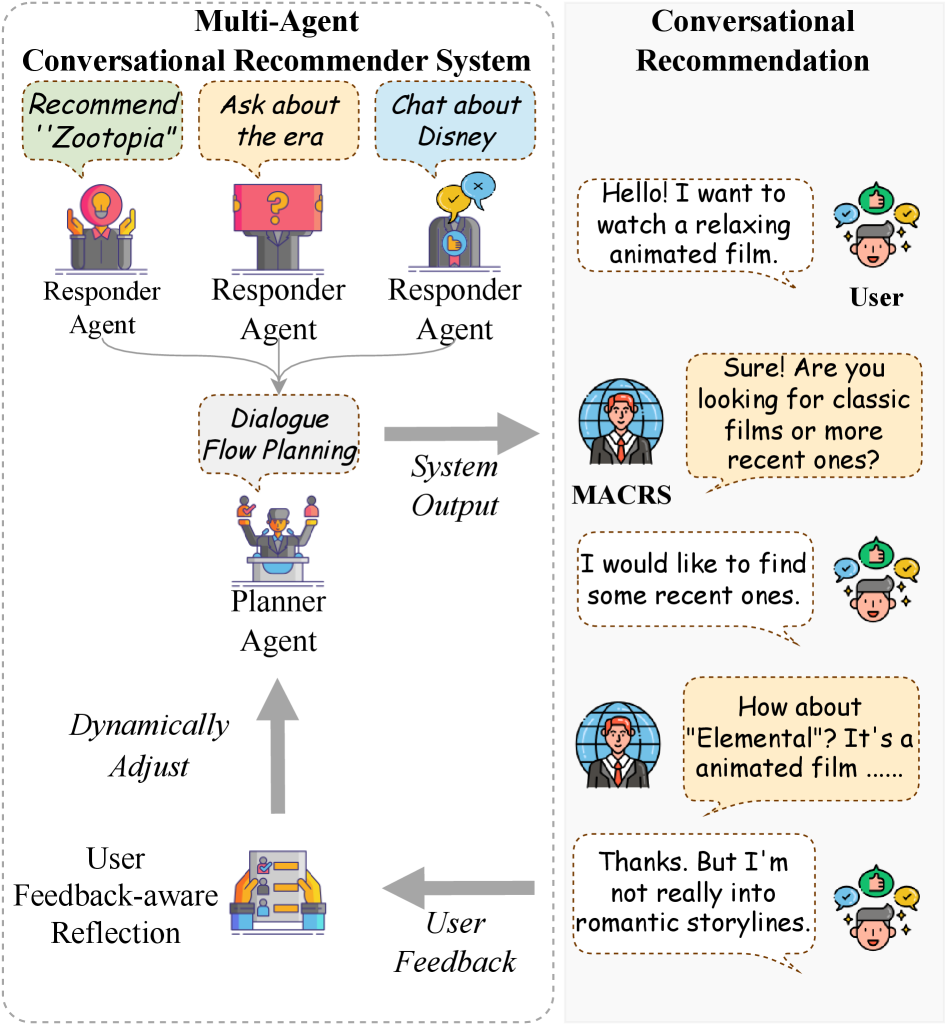
\includegraphics[width=\linewidth]{Chap2/images/crs_dialogue_example.png}
    \caption{Ví dụ hội thoại nhiều lượt trong Hệ thống gợi ý hội thoại. Hệ thống chủ động đặt câu hỏi làm rõ sở thích, cập nhật trạng thái hội thoại và đưa ra gợi ý kèm giải thích qua từng lượt tương tác \cite{fang2024multiagentconversationalrecommender}.}
    \label{fig:crs_dialogue_example}
\end{figure}

\section{Đồ thị Tri thức (Knowledge Graph - KG)}
Đồ thị tri thức (KG) biểu diễn tri thức thực thể dưới dạng tập hợp các bộ ba có hướng:
\begin{equation}
    \mathcal{G} = \{(h, r, t) \mid h, t \in \mathcal{E}, r \in \mathcal{R}\}
\end{equation}
trong đó $\mathcal{E}$ là tập thực thể (Phim, Đạo diễn, Thể loại, Diễn viên), $\mathcal{R}$ là tập quan hệ (đạo\_diễn\_bởi, thuộc\_thể\_loại, đóng\_vai), $h$ (head) và $t$ (tail) là thực thể gốc và đích, $r$ là quan hệ có hướng nối giữa chúng \cite{zhou2020improvingcrs}.

Trong ngữ cảnh CRS, dữ liệu tương tác người dùng - item thường rất thưa thớt (data sparsity). KG đóng ba vai trò bổ sung mà lịch sử tương tác đơn thuần không thể cung cấp:
\begin{itemize}
    \item \textbf{Nguồn dữ liệu thực chứng (Grounding):} Mọi thực thể được gợi ý đều có thể kiểm tra sự tồn tại trực tiếp trong KG, là nền tảng để loại bỏ hallucination từ LLM.
    \item \textbf{Suy luận đa bước (Multi-hop Reasoning):} Duyệt qua các cạnh đồ thị ở độ sâu $> 1$ cho phép phát hiện sở thích tiềm ẩn mà lịch sử tương tác trực tiếp không thể hiện (ví dụ: Phim $\rightarrow$ Diễn viên $\rightarrow$ Phim khác cùng diễn viên).
    \item \textbf{Nền tảng cho Truy xuất lai (Hybrid Retrieval):} KG hiện đại lưu trữ song song cả liên kết cấu trúc và vector nhúng (embeddings) của nội dung văn bản (tóm tắt cốt truyện, mô tả thực thể), cho phép kết hợp truy xuất ngữ nghĩa và truy xuất đồ thị trong cùng một hệ thống.
\end{itemize}

Hình \ref{fig:kg_structure_bg} minh họa cụ thể cách một node Phim được tổ chức trong KG, với các cạnh có hướng nối tới các thực thể liên quan như Đạo diễn, Diễn viên và Thể loại, thể hiện trực quan cấu trúc bộ ba $(h, r, t)$ được định nghĩa ở trên.

\begin{figure}[htbp]
    \centering
    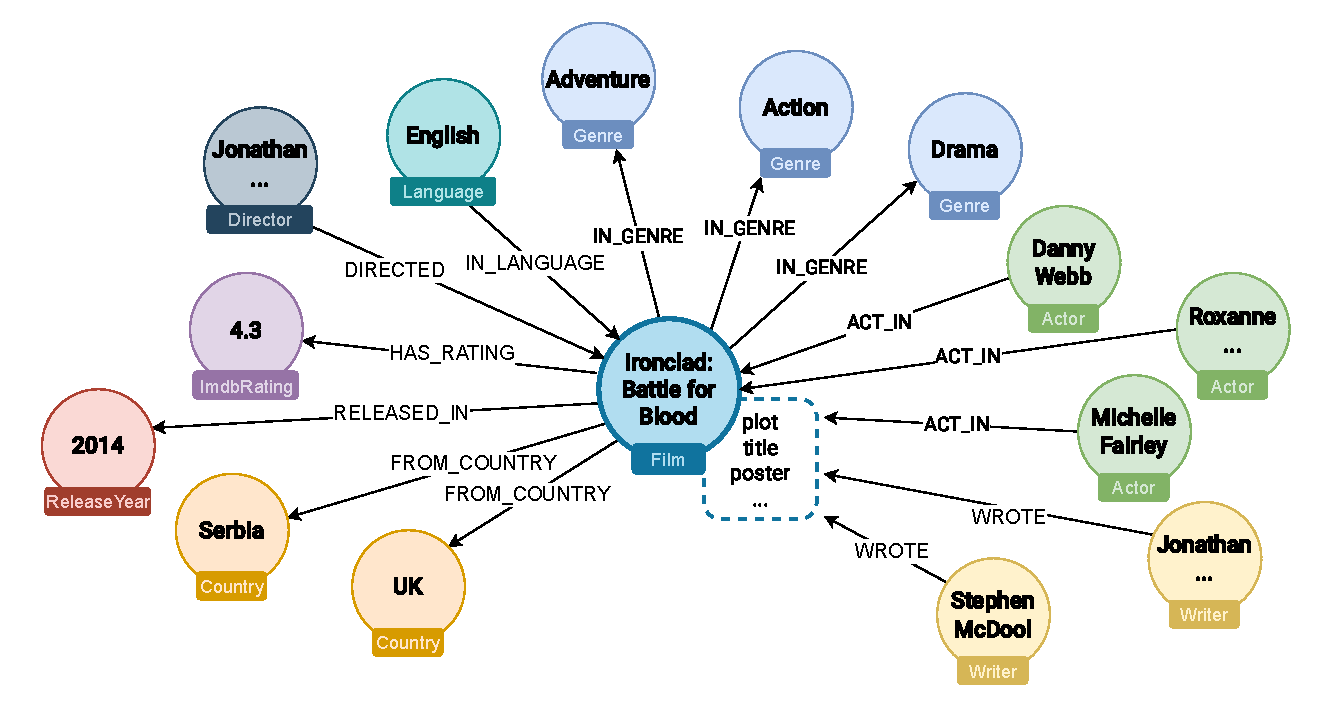
\includegraphics[width=0.75\linewidth]{Chap3/images/KG_node.pdf}
    \caption{Ví dụ cấu trúc một node Phim trong Đồ thị tri thức, liên kết với các thực thể Đạo diễn, Diễn viên, Thể loại và các thuộc tính định lượng. Mỗi bộ ba $(h, r, t)$ biểu diễn một quan hệ có hướng giữa hai thực thể trong đồ thị.}
    \label{fig:kg_structure_bg}
\end{figure}

\section{Mô hình Ngôn ngữ Lớn (LLMs) và Kỹ thuật RAG}

\subsection{Mô hình Ngôn ngữ Lớn (LLMs)}
LLM là các mô hình Transformer được huấn luyện trên khối lượng văn bản khổng lồ, có khả năng hiểu và sinh ngôn ngữ tự nhiên theo ngữ cảnh \cite{min2023recent}. Trong hệ thống CRS, LLM đảm nhận ba chức năng chính: (1) phân tích ý định và trích xuất ràng buộc từ lịch sử hội thoại, (2) suy luận về độ phù hợp của các ứng viên, và (3) sinh phản hồi ngôn ngữ tự nhiên \cite{zhao2024recommender}.

Hạn chế căn bản của LLM trong CRS là \textit{hallucination}: vì sinh văn bản theo phân phối xác suất, LLM có thể tự tạo ra các thực thể không tồn tại (phim bịa, đạo diễn sai) nhưng hoàn toàn hợp lý về mặt ngôn ngữ. Đây là lý do cần neo giữ (ground) đầu ra của LLM vào một nguồn dữ liệu thực chứng bên ngoài, vai trò mà KG đảm nhận trong hệ thống ARGOS.

\subsection{Kỹ thuật RAG (Retrieval-Augmented Generation)}
RAG giải quyết hạn chế của LLM bằng cách tách biệt lưu trữ tri thức (trong cơ sở dữ liệu ngoài) khỏi năng lực suy luận (của LLM) \cite{singh2026agenticretrievalaugmentedgenerationsurvey}. Thay vì học thuộc dữ liệu vào trọng số, LLM nhận tri thức liên quan theo thời gian thực qua hai pha:
\begin{enumerate}
    \item \textbf{Truy xuất (Retrieval):} Dựa trên truy vấn $q$, tìm kiếm tập tài liệu/thực thể $D$ liên quan từ kho dữ liệu ngoài (KG, vector database).
    \item \textbf{Sinh có điều kiện (Conditioned Generation):} LLM sinh phản hồi dựa trên $q$ và $D$ kết hợp, câu trả lời được neo giữ vào dữ liệu thực chứng thay vì chỉ dựa vào phân phối tham số.
\end{enumerate}

Luồng hoạt động tổng thể của pipeline RAG được minh họa trong Hình \ref{fig:rag_pipeline}.

\begin{figure}[htbp]
    \centering
    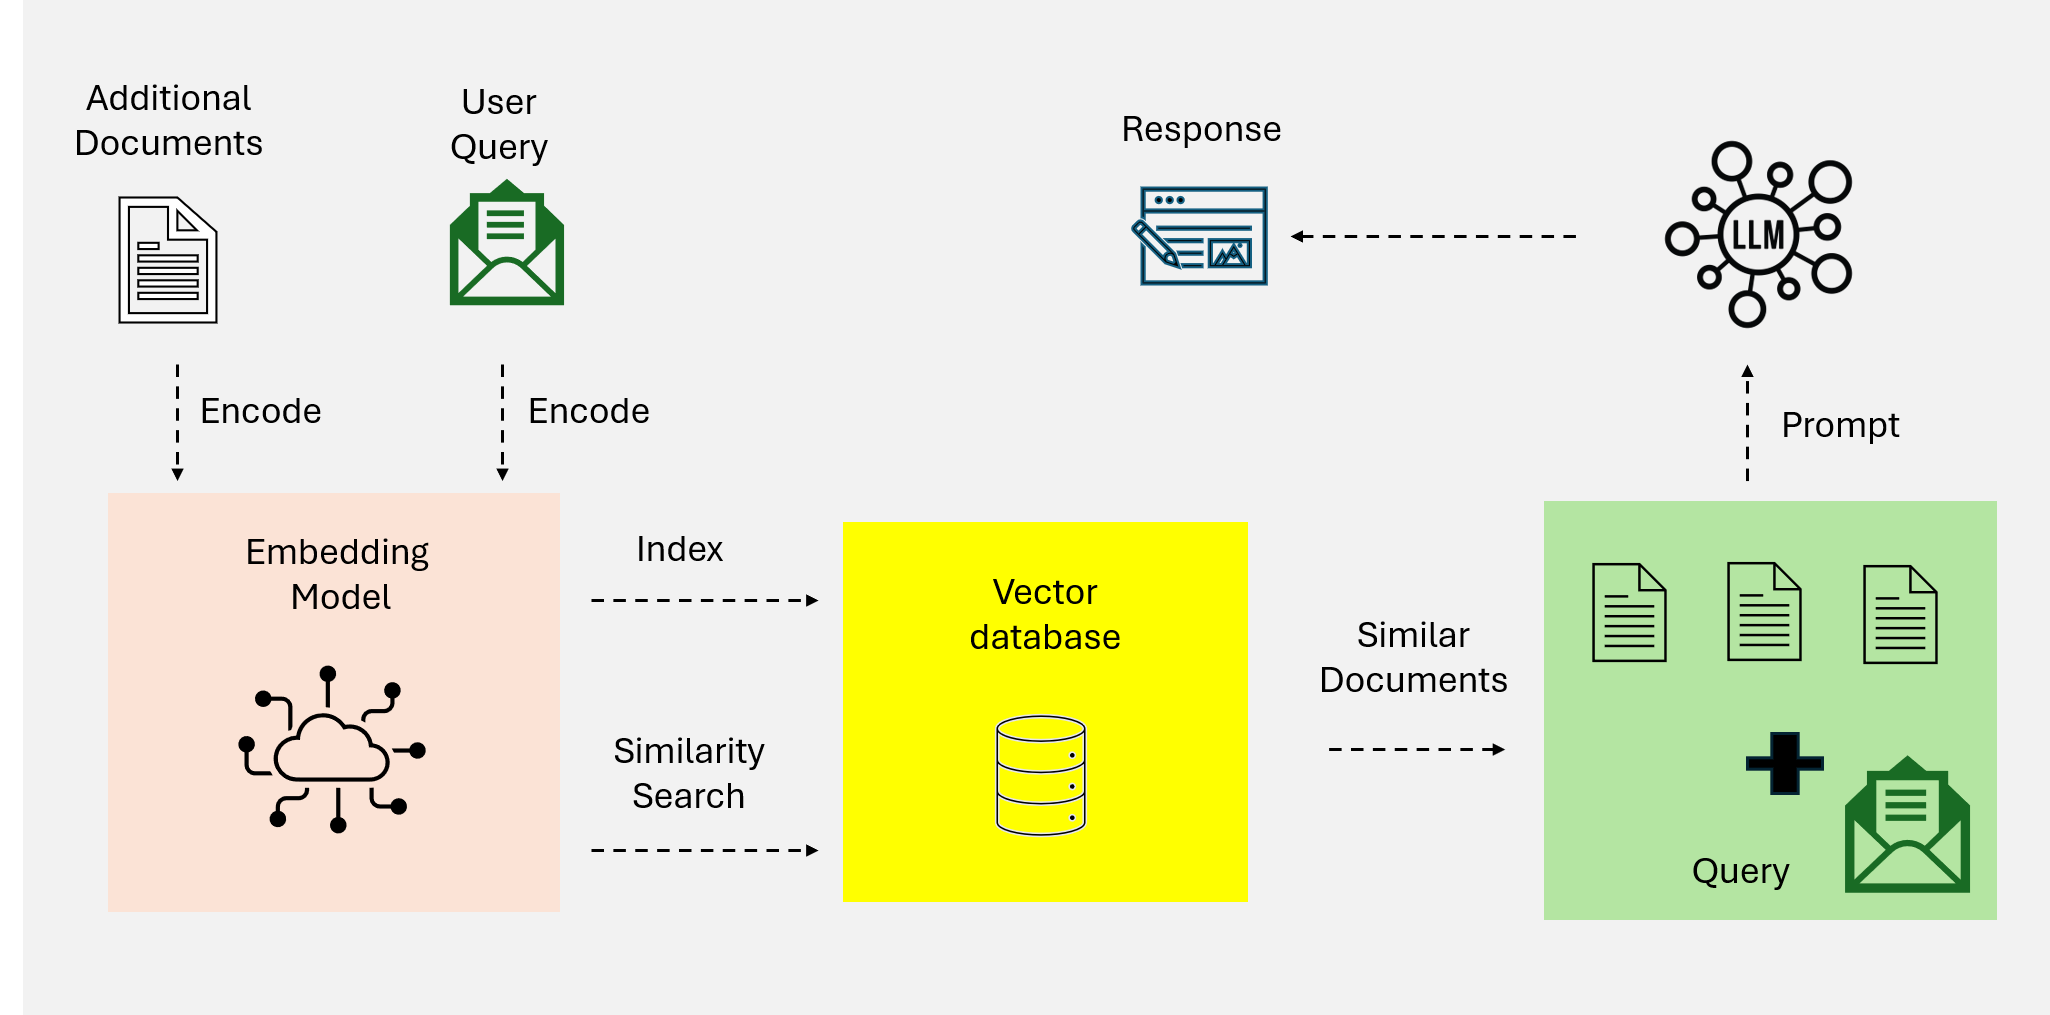
\includegraphics[width=\linewidth]{Chap2/images/rag_pipeline.png}
    \caption{Pipeline RAG cơ bản gồm ba giai đoạn: \textit{Retrieval} (truy xuất tài liệu liên quan từ kho dữ liệu ngoài), \textit{Augmentation} (tích hợp tài liệu vào ngữ cảnh) và \textit{Generation} (LLM sinh câu trả lời được neo giữ vào dữ liệu thực chứng) \cite{singh2026agenticretrievalaugmentedgenerationsurvey}.}
    \label{fig:rag_pipeline}
\end{figure}

RAG đặc biệt phù hợp với bài toán CRS vì ba lý do thực tiễn: (i) danh mục item thay đổi liên tục: RAG chỉ cần cập nhật KG mà không cần fine-tune lại LLM; (ii) mỗi gợi ý đều cần có cơ sở thực chứng: đường dẫn truy xuất của RAG cung cấp trực tiếp khả năng giải thích (explainability); (iii) chi phí thấp hơn đáng kể so với fine-tuning khi quy mô dữ liệu lớn.

\section{Kiến trúc Hệ thống Đa tác tử (Multi-Agent System) và ReAct}

\subsection{Hệ thống Đa tác tử dựa trên LLM}
Kiến trúc đa tác tử dựa trên LLM phân tách một hệ thống phức tạp thành nhiều tác tử (agents) tự trị, mỗi tác tử chuyên trách một nhiệm vụ cụ thể với prompt riêng và quyền truy cập vào các công cụ được chỉ định \cite{xi2023rise}. Nghiên cứu gần đây cho thấy cách tiếp cận này vượt trội so với kiến trúc đơn tác tử trong các bài toán đòi hỏi phân tích đa chiều, tự sửa lỗi và phối hợp giữa các nguồn thông tin dị dạng, đặc điểm phù hợp với tính chất phức tạp của hội thoại gợi ý thực tế.

\subsection{Vòng lặp ReAct (Reasoning and Acting)}
ReAct \cite{yao2022react} là framework cho phép tác tử xen kẽ giữa suy luận (Thought) và hành động tương tác với môi trường (Action-Observation) trong một vòng lặp liên tục:
\begin{itemize}
    \item \textbf{Thought:} Tác tử phân tích trạng thái hiện tại và lập kế hoạch bước tiếp theo.
    \item \textbf{Action:} Gọi công cụ cụ thể (truy vấn KG, gọi API) với tham số phù hợp.
    \item \textbf{Observation:} Nhận kết quả từ công cụ, cập nhật ngữ cảnh và lặp lại.
\end{itemize}

Hình \ref{fig:react_loop} so sánh trực quan vòng lặp ReAct với các phương pháp prompting khác, làm rõ cách xen kẽ giữa Thought và Action-Observation tạo nên khả năng tự điều chỉnh mà các phương pháp đơn thuần không có.

\begin{figure}[htbp]
    \centering
    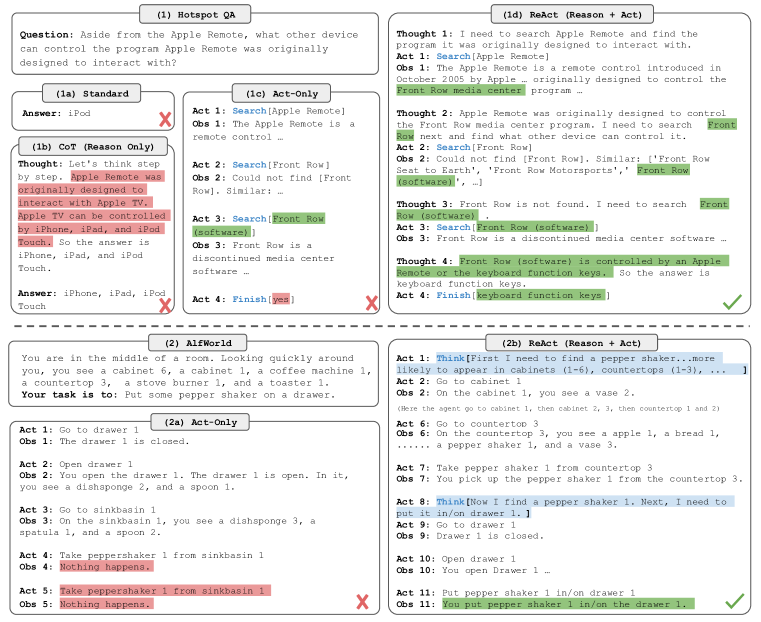
\includegraphics[width=\linewidth]{Chap2/images/react_loop.png}
    \caption{So sánh các phương pháp prompting LLM: Standard, Chain-of-Thought, Act-only và \textbf{ReAct}. ReAct xen kẽ giữa suy luận (Thought) và hành động tương tác với môi trường (Action-Observation), cho phép tác tử tự điều chỉnh chiến lược dựa trên phản hồi từ môi trường \cite{yao2022react}.}
    \label{fig:react_loop}
\end{figure}

ReAct phù hợp đặc biệt với bài toán CRS vì bản chất tương tác đa lượt của hội thoại đòi hỏi hệ thống phải liên tục quan sát, điều chỉnh, hành động trong vòng lặp, chứ không thể xử lý một lần rồi kết thúc như pipeline tĩnh. Cụ thể, khi một bước truy xuất KG thất bại, ReAct cho phép tác tử nhận biết sự cố qua Observation, suy luận nguyên nhân qua Thought tiếp theo, và thử chiến lược truy xuất khác qua Action mới, thay vì dừng hẳn và trả về kết quả rỗng. Đây chính xác là cơ chế mà các pipeline tĩnh đang thiếu.

\section{Bộ dữ liệu thực nghiệm}

Toàn bộ quá trình đánh giá trong khóa luận sử dụng hai bộ dữ liệu hội thoại chuẩn của lĩnh vực CRS:

\textbf{ReDial} \cite{li2018towards} là bộ dữ liệu hội thoại gợi ý phim tiếng Anh được thu thập qua Amazon Mechanical Turk, gồm hơn 10.000 hội thoại đa lượt giữa người hỏi và người trả lời. Mỗi hội thoại chứa ít nhất một lượt gợi ý phim với nhãn xác nhận (accepted/rejected), tạo thành ground truth rõ ràng cho đánh giá Recall@K.

\textbf{INSPIRED} \cite{hayati-etal-2020-inspired} là bộ dữ liệu hội thoại gợi ý phim tập trung vào chiến lược thuyết phục xã hội (social influence strategies), gồm 1.001 hội thoại với ngôn ngữ tự nhiên, cảm xúc và phong cách giao tiếp đa dạng hơn ReDial. Bộ dữ liệu này kiểm tra khả năng hiểu ngôn ngữ linh hoạt và hội thoại phi cấu trúc của hệ thống.

Hai bộ dữ liệu bổ sung cho nhau: ReDial đánh giá hiệu năng ở quy mô lớn với phân phối cân bằng, còn INSPIRED kiểm tra khả năng xử lý các truy vấn cảm xúc và ngôn ngữ đời thường. Giao thức đánh giá chi tiết (chiến lược lấy mẫu, kiểm định thống kê) được trình bày trong Chương 5.

\section{Các phương pháp đánh giá hệ thống (Evaluation Metrics)}
Nghiên cứu này sử dụng thang đo tiêu chuẩn \textbf{Recall@K} trong lĩnh vực gợi ý để đánh giá module Recommendation của ARGOS. Thang đo này phù hợp với bài toán CRS vì mỗi lượt hội thoại thường chỉ có một mục ground truth duy nhất, nên việc đo tỷ lệ xuất hiện trong top-K là chỉ số đánh giá trực tiếp và có ý nghĩa nhất.

\textbf{Recall@K} đo tỷ lệ item mục tiêu (ground truth) xuất hiện trong top-K gợi ý. Ký hiệu $V_u$ là tập item thực tế người dùng quan tâm, $R_u@K$ là top-K gợi ý của hệ thống:
\begin{equation}
    \text{Recall@K} = \frac{1}{|U|} \sum_{u \in U} \frac{|R_u@K \cap V_u|}{|V_u|}
\end{equation}

Thang đo được tính tại bốn ngưỡng $K \in \{1, 5, 10, 50\}$ trên hai bộ dữ liệu chuẩn ReDial \cite{li2018towards} và INSPIRED \cite{hayati-etal-2020-inspired}, nhất quán với giao thức đánh giá của các hệ thống SOTA được đối sánh trong Chương 5.

\section*{Kết luận chương}

Chương 2 đã thiết lập bốn nhóm kiến thức cốt lõi phục vụ cho việc hiểu và đánh giá hệ thống ARGOS. Bài toán CRS xác lập không gian vấn đề với hai nhiệm vụ song song mà ARGOS phải giải quyết. Đồ thị tri thức là nguồn dữ liệu thực chứng trung tâm, đảm bảo mọi gợi ý đều có cơ sở kiểm chứng và là nền tảng cho Hybrid Retrieval. LLM kết hợp RAG cung cấp năng lực suy luận ngôn ngữ mà không cần fine-tuning khi dữ liệu thay đổi. Kiến trúc đa tác tử với ReAct là mô hình tổ chức cho phép thiết lập vòng lặp phản hồi nội bộ, thành phần then chốt mà các hệ thống RAG tĩnh đang thiếu, và là nền tảng kỹ thuật của ARGOS.

Chương 3 tiếp theo phân tích chi tiết mô hình tiền đề GRACE, nơi RAG kết hợp KG lần đầu được áp dụng vào CRS của chính tác giả, để định lượng chính xác các điểm nghẽn mà ARGOS cần khắc phục.


% ----------------------CHƯƠNG 3----------------------
\chapter{Nghiên cứu tiền đề: Hệ thống GRACE}\label{chap:grace_baseline}

Chương này phân tích chi tiết hệ thống \textit{GRACE} (Graph-Reasoning Augmented Conversational Engine), nghiên cứu tiền đề của chính tác giả đã được công bố tại hội nghị quốc tế SOICT 2025 \cite{phan2025grace}. Thay vì chỉ tóm tắt lại nội dung bài báo, chương tập trung làm rõ từng thành phần kỹ thuật cụ thể và chỉ ra các giới hạn cấu trúc mà GRACE chưa giải quyết được, đây là cơ sở trực tiếp để đề xuất hệ thống ARGOS trong chương tiếp theo.

\section{Tổng quan kiến trúc GRACE}

GRACE được thiết kế theo mô hình hai giai đoạn công nghiệp tiêu chuẩn: Tạo ứng viên (Candidate Generation) và Xếp hạng lại (Re-ranking). Toàn bộ quy trình hoạt động theo cơ chế đường ống tĩnh (Static Pipeline) và không yêu cầu tinh chỉnh (fine-tune) trọng số của bất kỳ mô hình ngôn ngữ nào.

\begin{figure}[H]
    \centering
    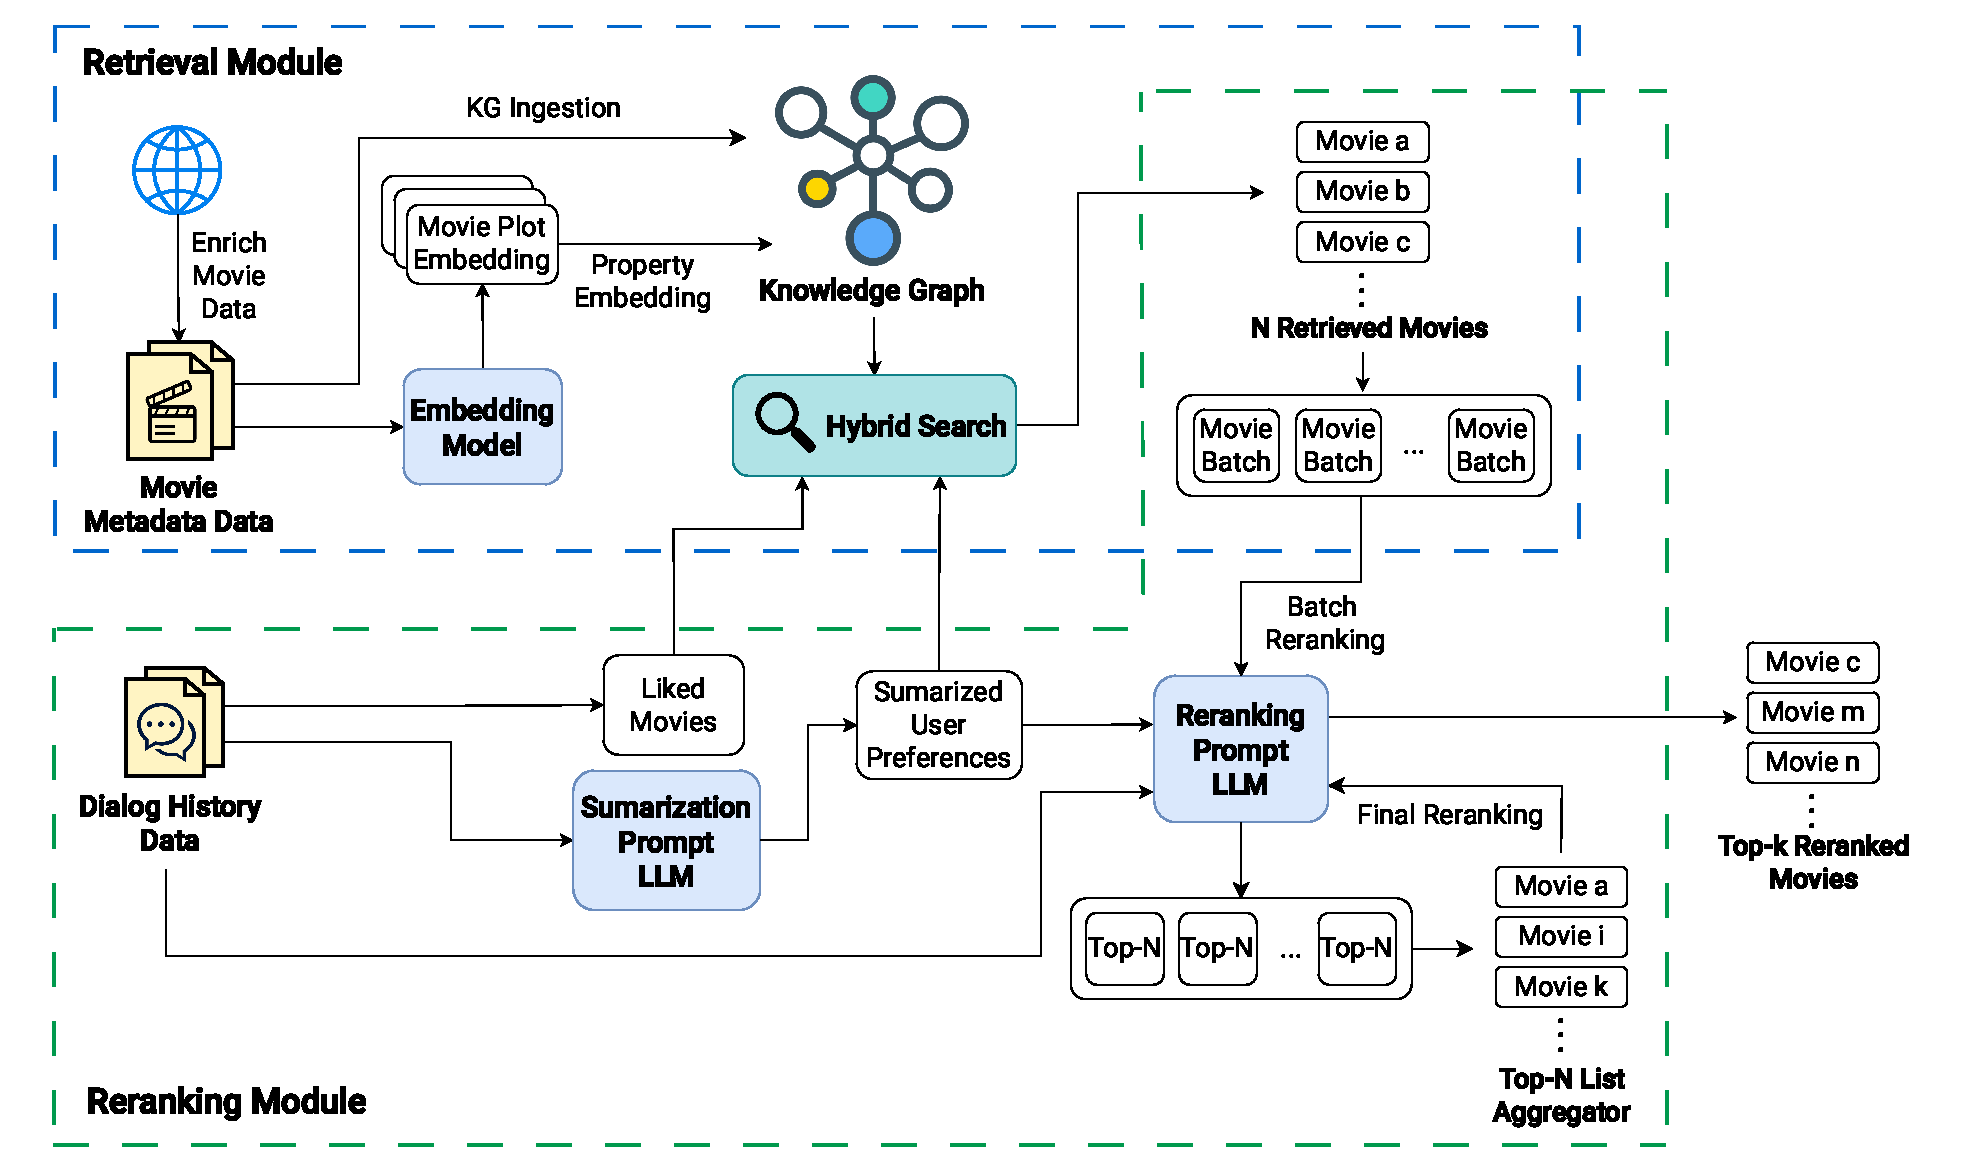
\includegraphics[width=\linewidth]{Chap3/images/grace.pdf}
    \caption{Tổng quan kiến trúc hệ thống tiền đề GRACE, bao gồm hai module chính: LLM Retriever và LLM Re-ranker.}
    \label{fig:grace_framework}
\end{figure}

Như minh họa trong Hình \ref{fig:grace_framework}, luồng hoạt động của GRACE gồm bốn bước tuần tự: (1) LLM tóm tắt lịch sử hội thoại thành một hồ sơ sở thích (Preference Profile); (2) ba chiến lược truy xuất song song (ngữ nghĩa, nội dung, đồ thị) tạo ra tập ứng viên; (3) các tập được hợp nhất và xếp hạng bằng Weighted Reciprocal Rank Fusion; (4) Generative LLM đánh giá lại và chọn ra kết quả cuối cùng. Kiến trúc này đảm bảo mọi thực thể trong tập ứng viên đều tồn tại trong KG vì chúng được truy xuất trực tiếp — loại trừ khả năng LLM tự bịa ra phim không tồn tại. Tuy nhiên, pipeline không kiểm tra liệu các ứng viên này có thỏa mãn toàn bộ ràng buộc cứng mà người dùng đặt ra trong hội thoại (danh sách loại trừ, ngưỡng điểm đánh giá) hay không — đây là khoảng trống mà Critic Agent trong ARGOS được thiết kế để lấp đầy.

\section{Xây dựng Đồ thị tri thức (Knowledge Graph Construction)}

Hiệu quả của GRACE phụ thuộc trực tiếp vào cấu trúc của Đồ thị tri thức (KG). Đồ thị này thống nhất siêu dữ liệu có cấu trúc và biểu diễn ngữ nghĩa cốt truyện vào cùng một không gian truy vấn.

\begin{figure}[H]
    \centering
    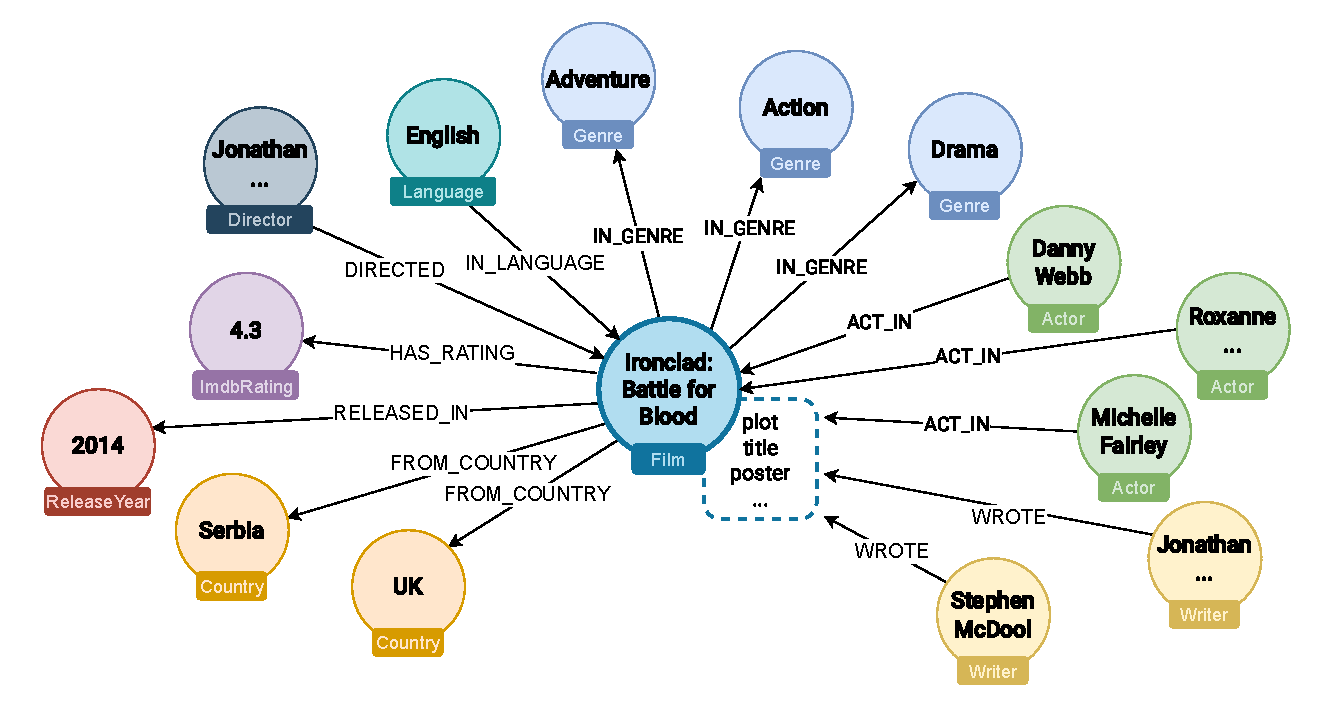
\includegraphics[width=0.85\linewidth]{Chap3/images/KG_node.pdf}
    \caption{Cấu trúc một node Phim (Film) trong Đồ thị tri thức. Node này liên kết trực tiếp với các thuộc tính (Năm, Điểm số, Thể loại) và các thực thể sáng tạo (Đạo diễn, Diễn viên).}
    \label{fig:kg_node}
\end{figure}

Quy trình xây dựng KG gồm ba bước:
\begin{itemize}
    \item \textbf{Tiền xử lý và Chuẩn hóa:} Chuyển đổi dữ liệu thô (năm phát hành, điểm số, thể loại, v.v.) sang định dạng sơ đồ thống nhất, xử lý các trường hợp nhập nhằng và trùng lặp thực thể.
    \item \textbf{Khởi tạo Đồ thị (Graph Construction):} Ánh xạ các thực thể phim và quan hệ vào cơ sở dữ liệu đồ thị Neo4j. Mỗi node Phim (\textit{Film}) được kết nối với các node phụ trợ như Thể loại (\textit{Genre}), Diễn viên (\textit{Actor}), Đạo diễn (\textit{Director}) (xem Hình \ref{fig:kg_node}).
    \item \textbf{Nhúng vector cốt truyện (Plot Embedding):} Gắn kèm vector nhúng dày đặc (dense embeddings) của đoạn tóm tắt cốt truyện trực tiếp vào node Phim tương ứng, cho phép truy vấn độ tương đồng cosine ngay bên trong đồ thị.
\end{itemize}

\section{Tóm tắt hội thoại và xây dựng Hồ sơ sở thích (Dialogue Summarization)}

Ký hiệu hội thoại đa lượt là $C = \{u_1, u_2, \dots, u_T\}$ với $u_t$ là phát ngôn thứ $t$. Mục tiêu của bước này là chưng cất $C$ thành một chuỗi văn bản tự nhiên duy nhất $\hat{P}$, gọi là Hồ sơ sở thích (Preference Profile), tóm tắt toàn bộ nhu cầu người tìm kiếm.

Thay vì dùng phương pháp điền khung (slot-filling) cứng nhắc với các trường có cấu trúc như \textit{likes, dislikes, constraints}, GRACE sử dụng một mẫu lời nhắc cố định \texttt{UserPreference} để buộc LLM sinh ra một đoạn văn xuôi mô tả duy nhất. Cách tiếp cận này tạo ra bản tóm tắt vừa đủ ngắn gọn, vừa dễ đọc, vừa thích hợp cho cả tìm kiếm từ khóa lẫn neo giữ vào KG, đồng thời giữ được tính chịu lỗi cao trước ngôn ngữ đời thường và hội thoại nhiễu.

\textit{Ví dụ từ tập dữ liệu ReDial:} cho đoạn hội thoại $C$ = [\textit{Respondent: "Hi, what kind of movies do you like?"}, \textit{Initiator: "I'm looking for a recommendation, I enjoyed A Nightmare on Elm Street (1984) when I was younger."}, \textit{Respondent: "Oh, you like scary movies?"}], LLM theo mẫu \texttt{UserPreference} sinh ra: $\hat{P}$ = \textit{"The seeker enjoys scary movies, particularly horror classics, and explicitly mentions A Nightmare on Elm Street (1984) as a movie they liked in the past. Their interest suggests a preference for suspenseful, frightening films, which can guide future recommendations."} Kết quả này cho thấy LLM không chỉ ghi nhận thực thể tường minh (tên phim) mà còn suy luận ra đặc trưng thể loại tiềm ẩn (genre affinity) từ ngữ cảnh.

Hồ sơ $\hat{P}$ sau đó được dùng làm đầu vào trực tiếp cho cả ba luồng truy xuất trong §\ref{sec:hybrid_retriever}.

\section{Module Truy xuất Lai (Hybrid Retriever)}\label{sec:hybrid_retriever}

Cơ chế truy xuất của GRACE kết hợp ba luồng độc lập để đảm bảo độ bao phủ (Recall) tối đa cho tập ứng viên, trong đó mỗi luồng bổ trợ cho nhau về loại thông tin khai thác được.

\subsection{Truy xuất ngữ nghĩa (Semantic Search)}
Hồ sơ sở thích được mã hóa thành vector truy vấn dày đặc $\mathbf{q}$, sau đó so sánh với vector cốt truyện $\mathbf{e}_f$ tại mỗi node phim trong KG qua độ tương đồng Cosine:
\begin{equation}
s_f = \cos(\mathbf{q}, \mathbf{e}_f) =
\frac{\mathbf{q} \cdot \mathbf{e}_f}{\lVert \mathbf{q}\rVert_2 \, \lVert \mathbf{e}_f\rVert_2}
\label{eq:similarity}
\end{equation}
trong đó $\lVert \mathbf{x} \rVert_2 = \sqrt{\sum_i x_i^2}$ là chuẩn Euclidean ($\ell_2$). Top-$m$ phim có $s_f$ cao nhất tạo thành tập kết quả $M_{\text{sem}}$. Luồng này đặc biệt hiệu quả khi nhu cầu người dùng mang tính chất thái, chủ đề hoặc cảm xúc khó biểu diễn bằng từ khóa cứng (Hình \ref{fig:semantic_retrieval}).

\begin{figure}[H]
    \centering
    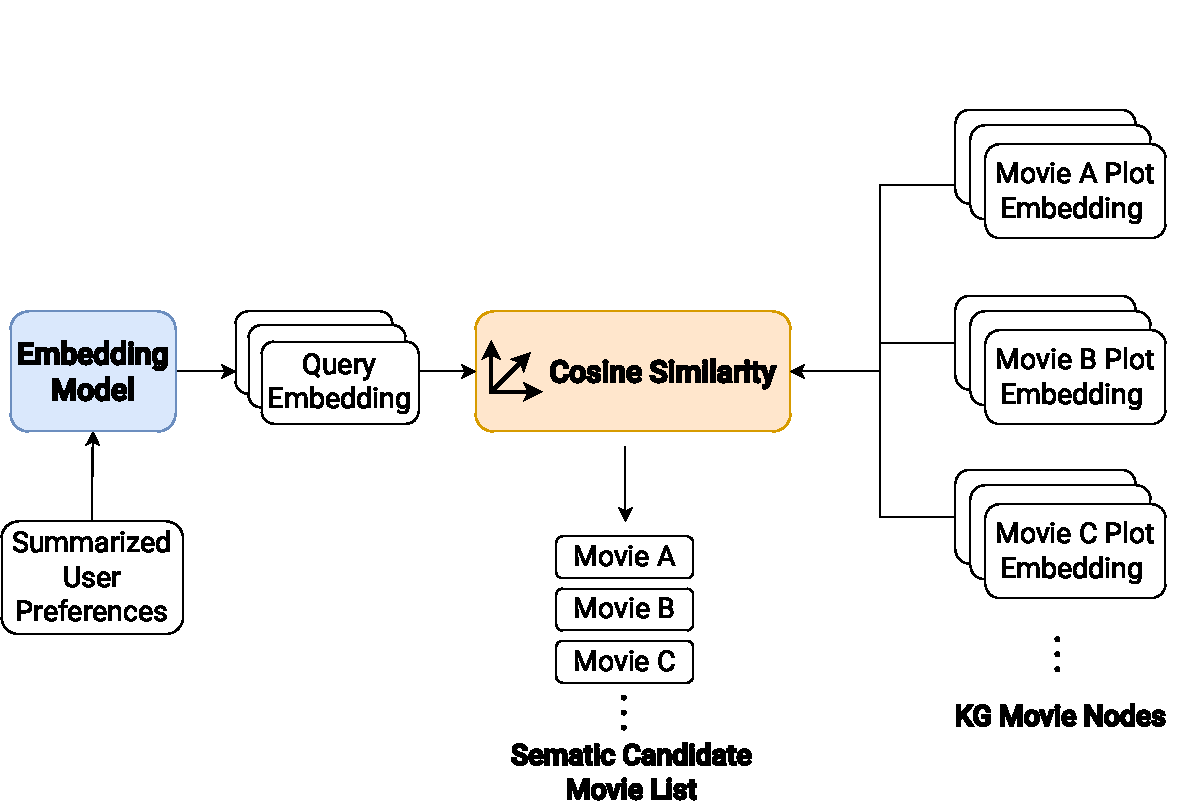
\includegraphics[width=0.85\linewidth]{Chap3/images/sem_retrieval.pdf}
    \caption{Quy trình truy xuất ngữ nghĩa dựa trên phép tính tương đồng Cosine giữa vector của câu truy vấn và vector cốt truyện phim.}
    \label{fig:semantic_retrieval}
\end{figure}

\subsection{Lọc theo nội dung (Content-based Filtering)}
Để thực thi các ràng buộc tường minh, ngữ cảnh hội thoại được chuyển đổi thành tập thể loại chuẩn hóa $G$ thông qua một bộ trích xuất LLM có ràng buộc (constrained LLM extractor), áp dụng ánh xạ từ đồng nghĩa (ví dụ: \textit{"science fiction"} $\mapsto$ \textit{"sci-fi"}), chuẩn hóa không phân biệt chữ hoa/thường, và chấp nhận nhãn ghép (compound labels). Khi $G$ không thể trích xuất đáng tin cậy, một bản đồ dự phòng keyword$\to$genre được dùng để đảm bảo độ phủ.

Mỗi phim $f$ với tập thể loại $\Gamma_f$ được đánh giá theo bộ giá trị xếp hạng từ điển (lexicographic tuple):
\begin{equation}
g_f = \big(|\Gamma_f \cap G|,\, r_f,\, y_f \big)\label{eq:enhanced_content_based}
\end{equation}
trong đó $|\Gamma_f \cap G|$ là số thể loại trùng khớp (ưu tiên tuyệt đối), $r_f$ là điểm IMDb, và $y_f$ là năm phát hành. Cách sắp xếp theo $y_f$ giảm dần mặc định ưu tiên phim mới hơn, một heuristic hợp lý trong phần lớn trường hợp nhưng có thể không phù hợp khi người dùng tìm phim cổ điển. Top-$m$ phim tạo thành tập $M_{\text{con}}$ (Hình \ref{fig:content_retrieval}).

\begin{figure}[H]
    \centering
    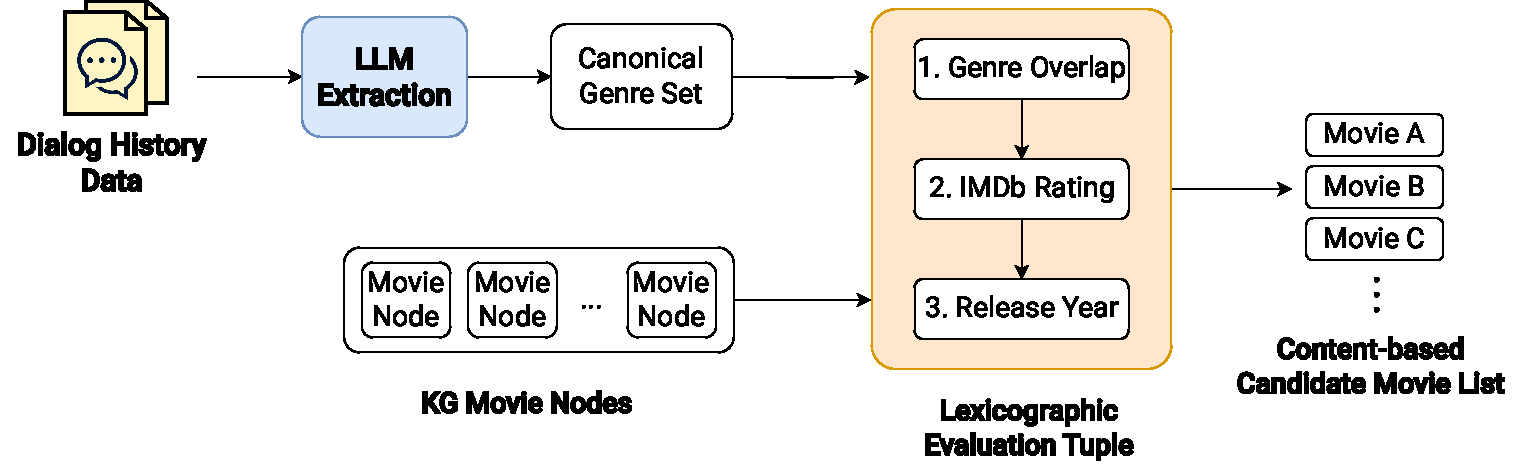
\includegraphics[width=0.85\linewidth]{Chap3/images/con_retrieval.pdf}
    \caption{Cơ chế lọc theo nội dung dựa trên các thuộc tính cứng (Thể loại, Năm sản xuất, Điểm số).}
    \label{fig:content_retrieval}
\end{figure}

\subsection{Mở rộng đồ thị (Graph Expansion - Collaborative)}
Xuất phát từ tập hạt giống (seed set) $L$ gồm các phim người dùng đã đề cập tích cực, thuật toán duyệt đồ thị dọc theo các cạnh liên kết với Diễn viên, Đạo diễn hoặc Biên kịch để tìm phim lân cận. Điểm số cộng tác cho phim ứng viên $f$ được tính:
\begin{equation}
S_{\text{col}}(f) = \sum_{s\in L} c(s,f) \label{eq:connection_count}
\end{equation}
trong đó $c(s,f)$ là số thực thể sáng tạo chia sẻ chung giữa phim hạt giống $s$ và phim ứng viên $f$. Các phim được sắp xếp theo tuple $\big(S_{\text{col}}(f), r_f\big)$ và top-$m$ tạo thành tập $M_{\text{col}}$ (Hình \ref{fig:collaborative_retrieval}).

\begin{figure}[H]
    \centering
    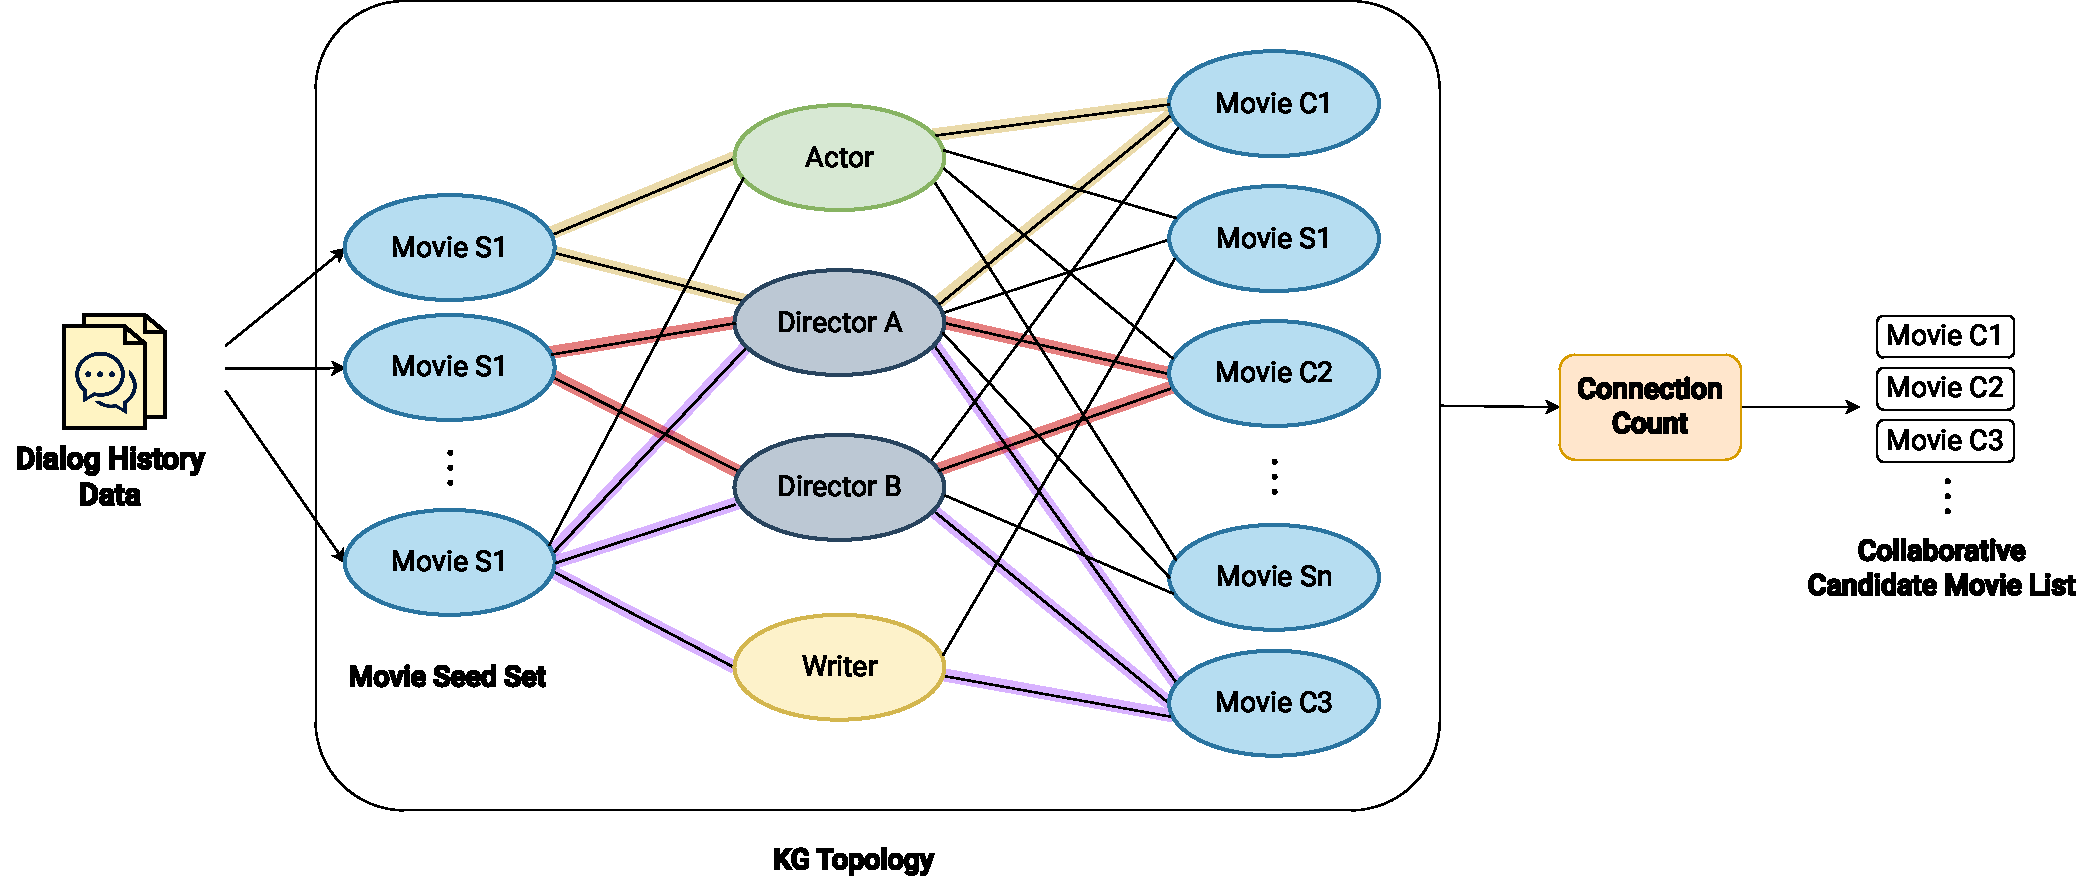
\includegraphics[width=0.85\linewidth]{Chap3/images/col_retrieval.pdf}
    \caption{Thuật toán mở rộng đồ thị dựa trên việc chia sẻ các node đội ngũ sáng tạo (Diễn viên, Đạo diễn).}
    \label{fig:collaborative_retrieval}
\end{figure}

\subsection{Cơ chế hợp nhất (Hybrid Integration)}
Đầu ra từ ba luồng trước tiên được gộp qua cơ chế loại bỏ trùng lặp ổn định (giữ nguyên thứ tự chèn):
\begin{equation}
M = \mathrm{StableDedup}(M_{\text{sem}} \cup M_{\text{con}} \cup M_{\text{col}})\label{eq:hybrid_integration}
\end{equation}
Tiếp theo, một bộ tiền xếp hạng tất định nhẹ (lightweight deterministic pre-ranker) theo thứ tự ưu tiên $(r_f, y_f)$ (điểm IMDb trước, năm phát hành sau) được áp dụng để lọc sơ bộ, loại bỏ ứng viên chất lượng thấp trước khi hợp nhất thứ hạng chính thức.

Các danh sách xếp hạng từ ba luồng sau đó được hợp nhất bằng thuật toán \textit{Weighted Reciprocal Rank Fusion} (WRRF) \cite{cormack2009reciprocal}:
\begin{equation}
\text{WRRF}(f) = \sum_{i \in \{\text{sem}, \text{con}, \text{col}\}} \frac{w_i}{k + \text{rank}_i(f)} \label{eq:wrrf}
\end{equation}
trong đó $w_i$ là trọng số của từng luồng (thực nghiệm: $w_{\text{sem}}=0.4$, $w_{\text{con}}=0.35$, $w_{\text{col}}=0.25$, được chọn để cân bằng giữa mức độ liên quan ngữ nghĩa, độ chính xác schema và đa dạng cộng tác), $\text{rank}_i(f)$ là thứ hạng của phim $f$ trong luồng $i$ (phim không có mặt được gán thứ hạng ảo lớn), và $k=60$ là hằng số làm mượt theo chuẩn RRF.

Đáng lưu ý, các trọng số $w_i$ được xác định thực nghiệm và \textit{cố định trong suốt quá trình vận hành}, bất kể hình thái ngôn ngữ của truy vấn. Đây là giới hạn thiết kế sẽ được phân tích tại §\ref{sec:grace_bottleneck}. Tập ứng viên cuối cùng $M_{\text{final}}$ được sắp xếp giảm dần theo điểm WRRF và chuyển giao cho module Re-ranker.

\section{Module Xếp hạng lại bằng Generative LLM}

Module Re-ranker (Hình \ref{fig:reranker}) nhận vào ba thành phần từ giai đoạn truy xuất: hồ sơ sở thích $\hat{P}$, tập ứng viên $M_{\text{final}}$, và siêu dữ liệu đã làm giàu (cốt truyện, thể loại, diễn viên, điểm số) của từng ứng viên. Cách tiếp cận này neo giữ quyết định của LLM vào thuộc tính thực chứng thay vì chỉ dựa vào ngữ cảnh hội thoại phẳng (flat dialogue context).

\begin{figure}[H]
    \centering
    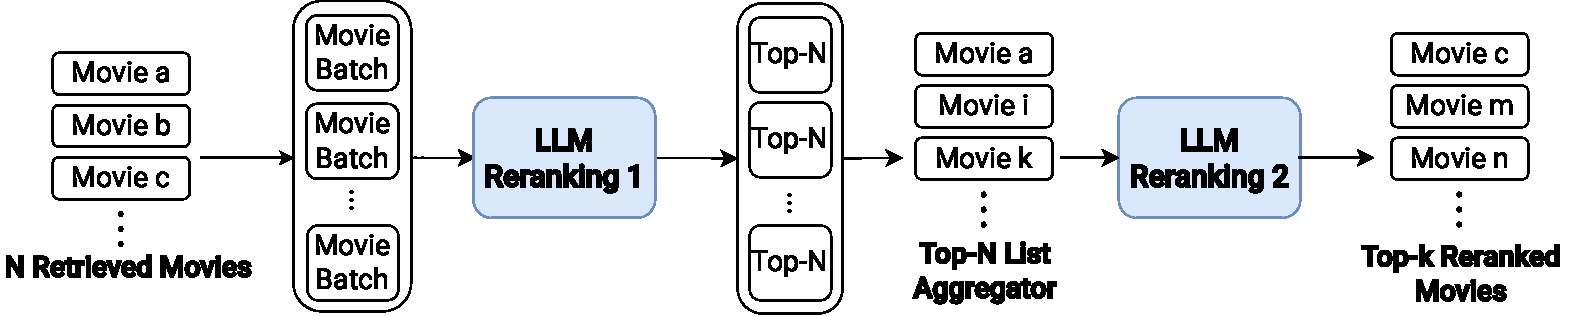
\includegraphics[width=0.85\linewidth]{Chap3/images/reranker.pdf}
    \caption{Kiến trúc Module Xếp hạng lại, sử dụng cơ chế batching để xử lý tập ứng viên lớn thông qua LLM.}
    \label{fig:reranker}
\end{figure}

Để xử lý giới hạn context window, GRACE giới thiệu kỹ thuật \textit{two-stage batching with shortlist fusion} kết hợp \textit{metadata augmentation}: (i) giai đoạn Batch Re-ranking chia $M_{\text{final}}$ thành các lô nhỏ, mỗi lô được LLM xếp hạng độc lập thành một shortlist; (ii) giai đoạn Final Re-ranking hợp nhất các shortlist và thực hiện một lượt đánh giá tổng hợp cuối để chọn ra top-K. Đây là kỹ thuật chưa được kết hợp đồng thời trong các hệ thống CRS trước đó như LLM-ReDial, UniCRS hay G-CRS.

Mô hình xuất ra một JSON object nghiêm ngặt chỉ chứa các phim từ tập ứng viên. Một validator độc lập kiểm tra tuân thủ schema, loại bỏ mục không hợp lệ, giải quyết trường hợp hòa (tie-breaking), và áp dụng cắt ngắn top-$k$ tất định. Cơ chế retry có giới hạn và sửa lỗi nhẹ đảm bảo hệ thống thoái hóa nhẹ nhàng (graceful degradation) thay vì thất bại hoàn toàn khi LLM trả về định dạng sai. Nhờ validator này, kết quả cuối cùng chỉ chứa các phim thuộc tập ứng viên đã được truy xuất từ KG — đảm bảo không có thực thể do LLM tự bịa ra. Giới hạn còn lại là validator chỉ kiểm tra tính hợp lệ schema của đầu ra, không đối chiếu ngược lại ràng buộc cứng của người dùng; điểm nghẽn này được giải quyết ở Chương 4.

\section{Phân tích điểm nghẽn mang tính cấu trúc}\label{sec:grace_bottleneck}

Mặc dù GRACE chứng minh được hiệu quả trong việc loại bỏ ảo giác và đạt kết quả cạnh tranh trên các bộ dữ liệu chuẩn (kết quả chi tiết tại Bảng \ref{tab:baseline_comparison}, Chương 5), kiến trúc Static Pipeline của nó bộc lộ ba điểm nghẽn có tính cấu trúc khi triển khai thực tế:

\begin{enumerate}
    \item \textbf{Tính phi linh hoạt của Pipeline (Pipeline Rigidity):} Luồng xử lý một chiều không có khả năng tự điều chỉnh khi một bước trung gian thất bại. Ví dụ điển hình: nếu LLM trong bước tóm tắt trích xuất nhầm thể loại từ hội thoại (diễn giải "phim căng thẳng" thành \textit{horror} thay vì \textit{thriller}), toàn bộ tập ứng viên từ luồng Content-based sẽ lệch hướng, nhưng pipeline không có cơ chế phát hiện và sửa lỗi này.

    \item \textbf{Thiếu điều phối trọng số động (Lack of Dynamic Weighting):} Trọng số WRRF cố định ($w_{\text{sem}}=0.4$, $w_{\text{con}}=0.35$, $w_{\text{col}}=0.25$) không phản ánh sự khác biệt về ngữ nghĩa giữa các loại truy vấn. Khi người dùng hỏi \textit{"phim gì có cùng diễn viên với Inception?"}, đây là truy vấn thuần đồ thị, do đó trọng số $w_{\text{col}}$ lẽ ra phải chiếm ưu thế tuyệt đối. Ngược lại, với yêu cầu \textit{"phim có không khí như Blade Runner"}, truy xuất ngữ nghĩa mới là kênh hữu ích. Pipeline tĩnh không phân biệt được hai tình huống này.

    \item \textbf{Chi phí và Độ trễ từ Generative LLM:} Việc dùng Generative LLM cho toàn bộ khâu re-ranking gây ra độ trễ đáng kể trong tương tác thời gian thực. Khi tập ứng viên lớn phải qua nhiều lô đánh giá, mỗi lô đều phát sinh một lần gọi API, tích lũy cả về chi phí lẫn latency, đặc biệt bất lợi khi cần phản hồi tức thì trong hội thoại.
\end{enumerate}

\section*{Kết luận chương}

Chương 3 đã phân tích chi tiết từng thành phần kỹ thuật của GRACE: từ cấu trúc KG, cơ chế tóm tắt hội thoại, ba luồng truy xuất lai, cho đến giai đoạn re-ranking bằng Generative LLM. Những thành tựu của GRACE trong việc loại bỏ ảo giác nhờ KG và cơ chế validator là cơ sở kỹ thuật quan trọng được ARGOS kế thừa. Tuy nhiên, ba điểm nghẽn được xác định (pipeline cứng nhắc, trọng số tĩnh và chi phí re-ranking) đặt ra yêu cầu rõ ràng cho kiến trúc kế tiếp: một hệ thống có khả năng tự điều chỉnh chiến lược và phản hồi nội bộ. Đây là nền tảng để Chương 4 trình bày kiến trúc đa tác tử \textbf{ARGOS}.


% ----------------------CHƯƠNG 4----------------------
% !TEX root = ../main.tex
\chapter{Kiến trúc đề xuất: Hệ thống Đa tác tử ARGOS}\label{chap:argos_proposed}

Chương này trình bày thiết kế và cơ chế vận hành của hệ thống \textbf{ARGOS} (Adaptive Reasoning and Graph Orchestration System). Các điểm nghẽn được xác định tại Chương 3 (thiếu cơ chế tự sửa lỗi, thiếu khả năng nới lỏng ràng buộc, và trọng số truy xuất cố định) được giải quyết bằng cách phân tách các chức năng thành năm tác tử chuyên biệt: Profiler, Graph Agent, Orchestrator, Critic và Relaxation Agent. Các tác tử này liên kết với nhau qua các vòng lặp phản hồi dựa trên mô hình ReAct, tạo nên một kiến trúc có khả năng tự phát hiện lỗi, điều chỉnh chiến lược truy xuất và khôi phục hội thoại khi gặp truy vấn quá khắt khe.

\section{Động lực chuyển đổi sang Vòng lặp phản hồi Đa tác tử (Multi-Agent Feedback Loop)}

Pipeline tuyến tính của GRACE xử lý mỗi truy vấn theo một chiều duy nhất: phân tích ý định → truy xuất → xếp hạng. Khi bước nào thất bại (truy vấn đồ thị trả về rỗng, hay toàn bộ ứng viên bị lọc bởi ràng buộc cứng), pipeline dừng lại và trả về kết quả trống mà không có cơ chế khắc phục. Sự vắng mặt của phản hồi nội bộ (internal feedback) khiến lỗi ở bước đầu lan truyền và khuếch đại qua các bước sau.

ARGOS giải quyết bằng mô hình tổ chức khác: mỗi chức năng cốt lõi được giao cho một tác tử chuyên biệt (Profiler, Graph Agent, Orchestrator, Critic, Relaxation) và các tác tử này giao tiếp qua tín hiệu phản hồi thay vì truyền dữ liệu một chiều. Khi Critic Agent phát hiện không đủ kết quả hợp lệ, nó không trả về lỗi mà phát tín hiệu kích hoạt Relaxation Agent, tác tử này tái cấu trúc ý định và khởi động lại vòng truy xuất. Tổng quan kiến trúc được minh họa trong Hình \ref{fig:argos_architecture}.

\begin{figure}[H]
    \centering
    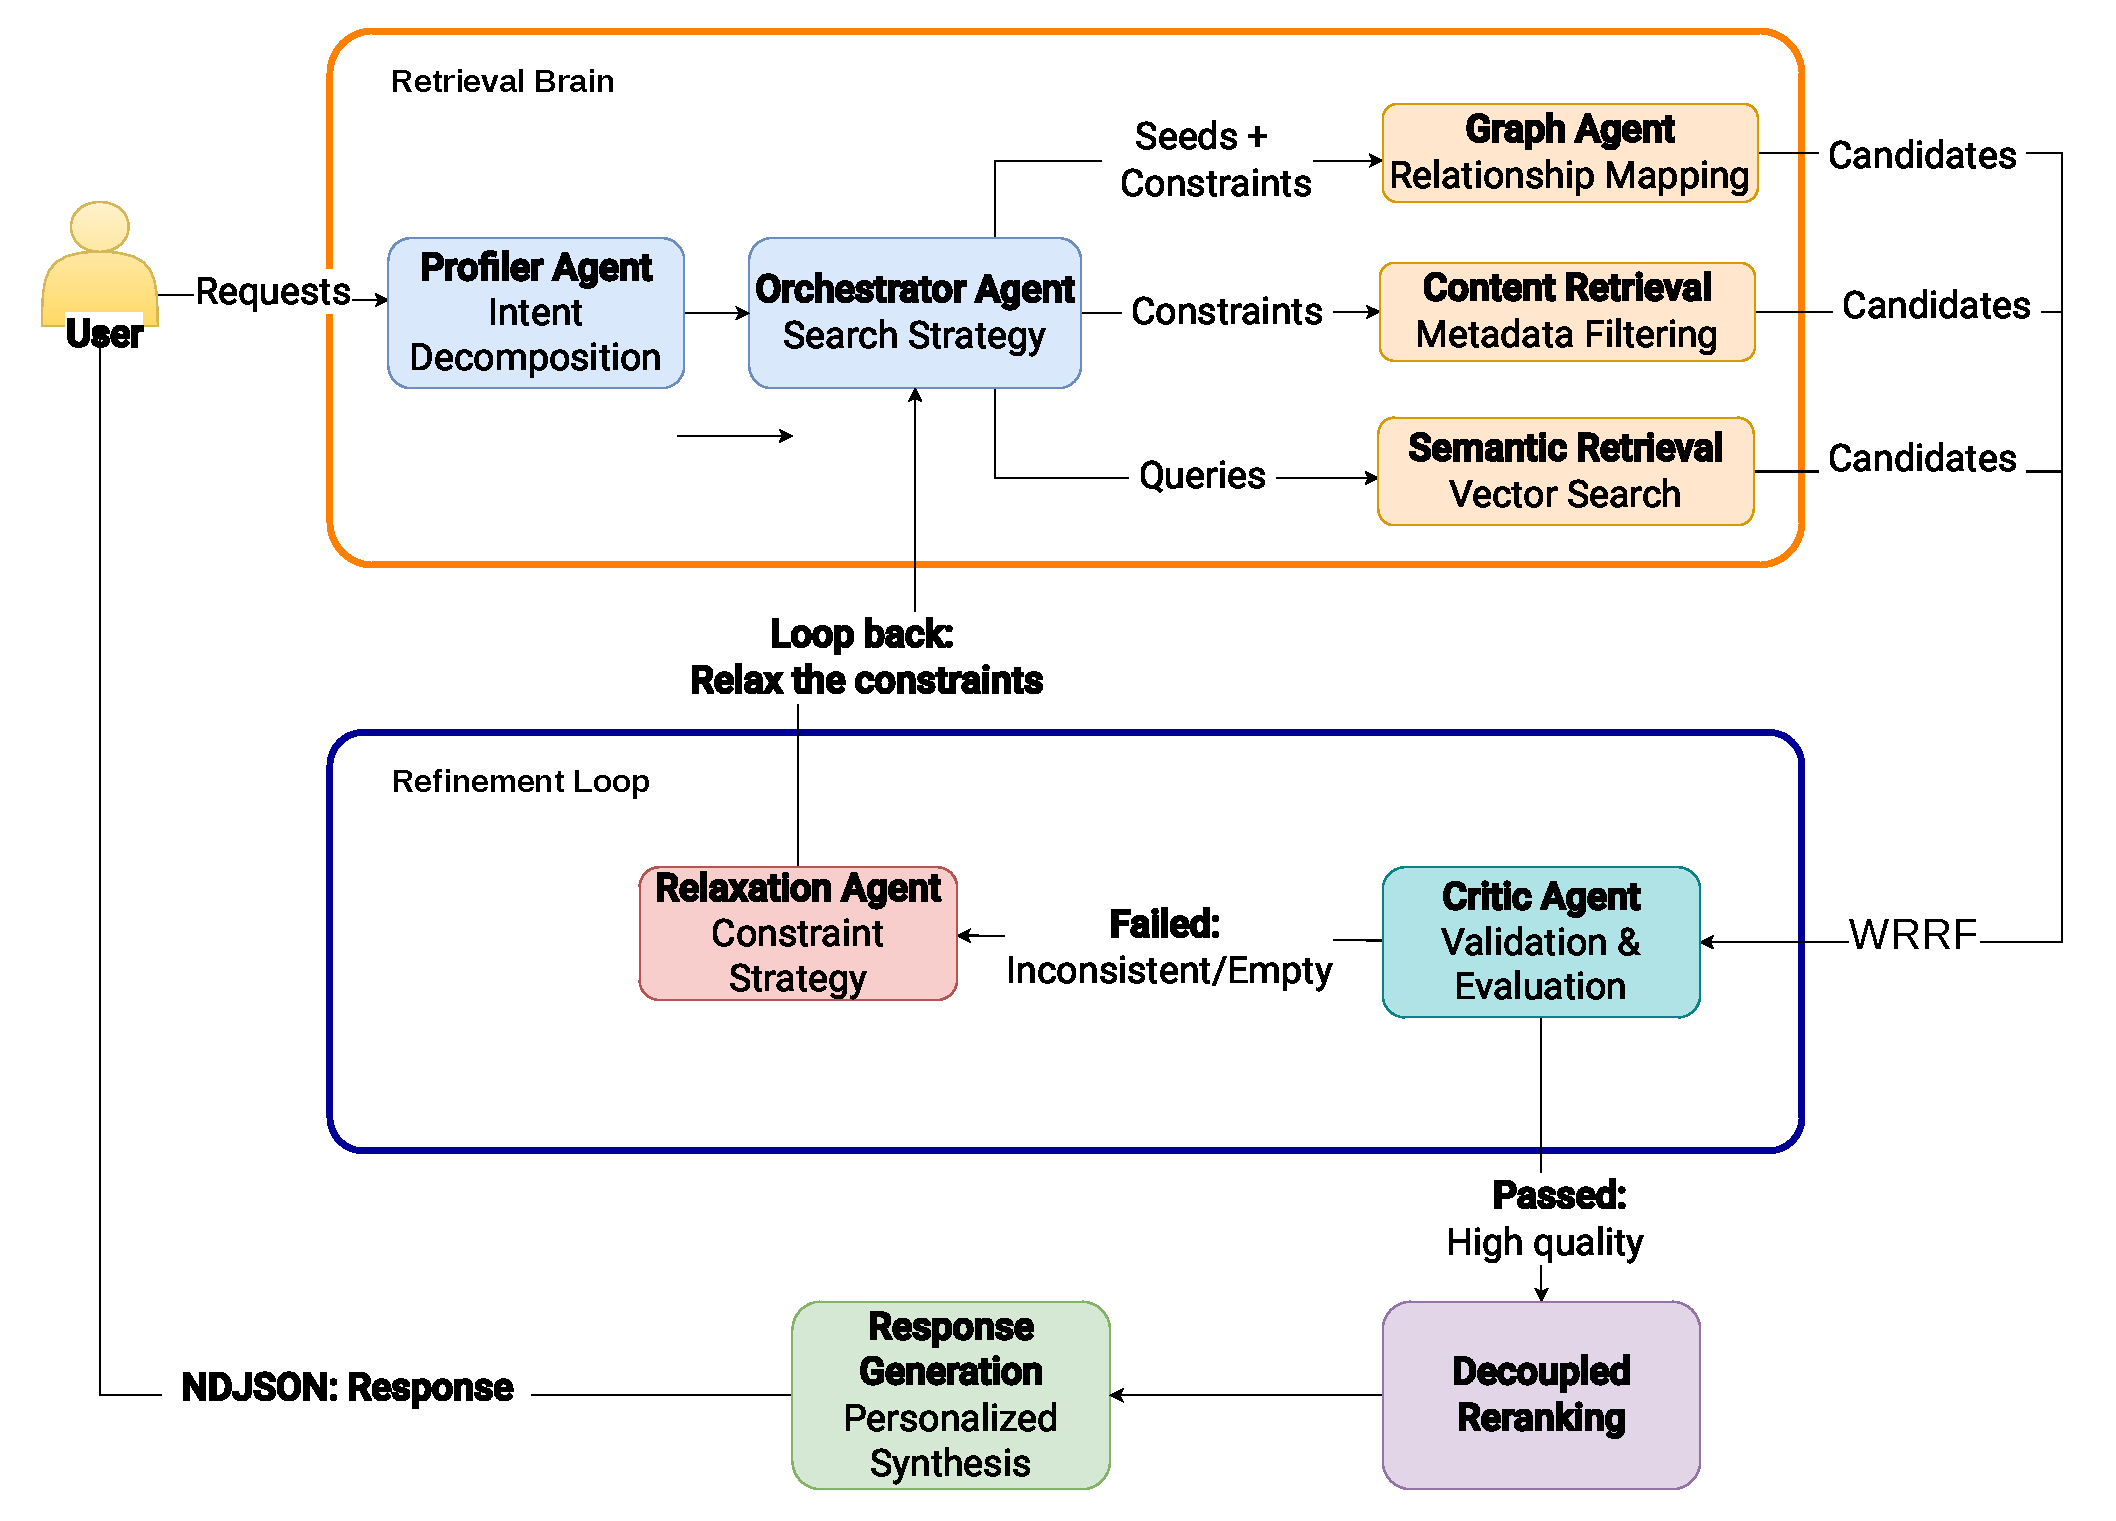
\includegraphics[width=\linewidth]{Chap4/images/argos_architecture.pdf}
    \caption{Kiến trúc tổng quan của hệ thống đa tác tử ARGOS. Khác với kiến trúc tĩnh, ARGOS đưa vào các vòng lặp phản hồi nội bộ (feedback loops) và cơ chế đánh giá lại trọng số động thông qua các Agent chuyên biệt.}
    \label{fig:argos_architecture}
\end{figure}

\section{Tác tử Hồ sơ (Profiler Agent) và Phân rã ý định}

Profiler Agent là tác tử đầu tiên trong chuỗi xử lý, chịu trách nhiệm chuyển hóa yêu cầu ngôn ngữ tự nhiên của người dùng thành các cấu trúc dữ liệu chuẩn hóa (Structured Output) để các tác tử sau có thể sử dụng nhất quán. Quá trình này gồm ba cơ chế cốt lõi, được minh họa tổng quan trong Hình \ref{fig:profiler_agent}.

\begin{figure}[H]
    \centering
    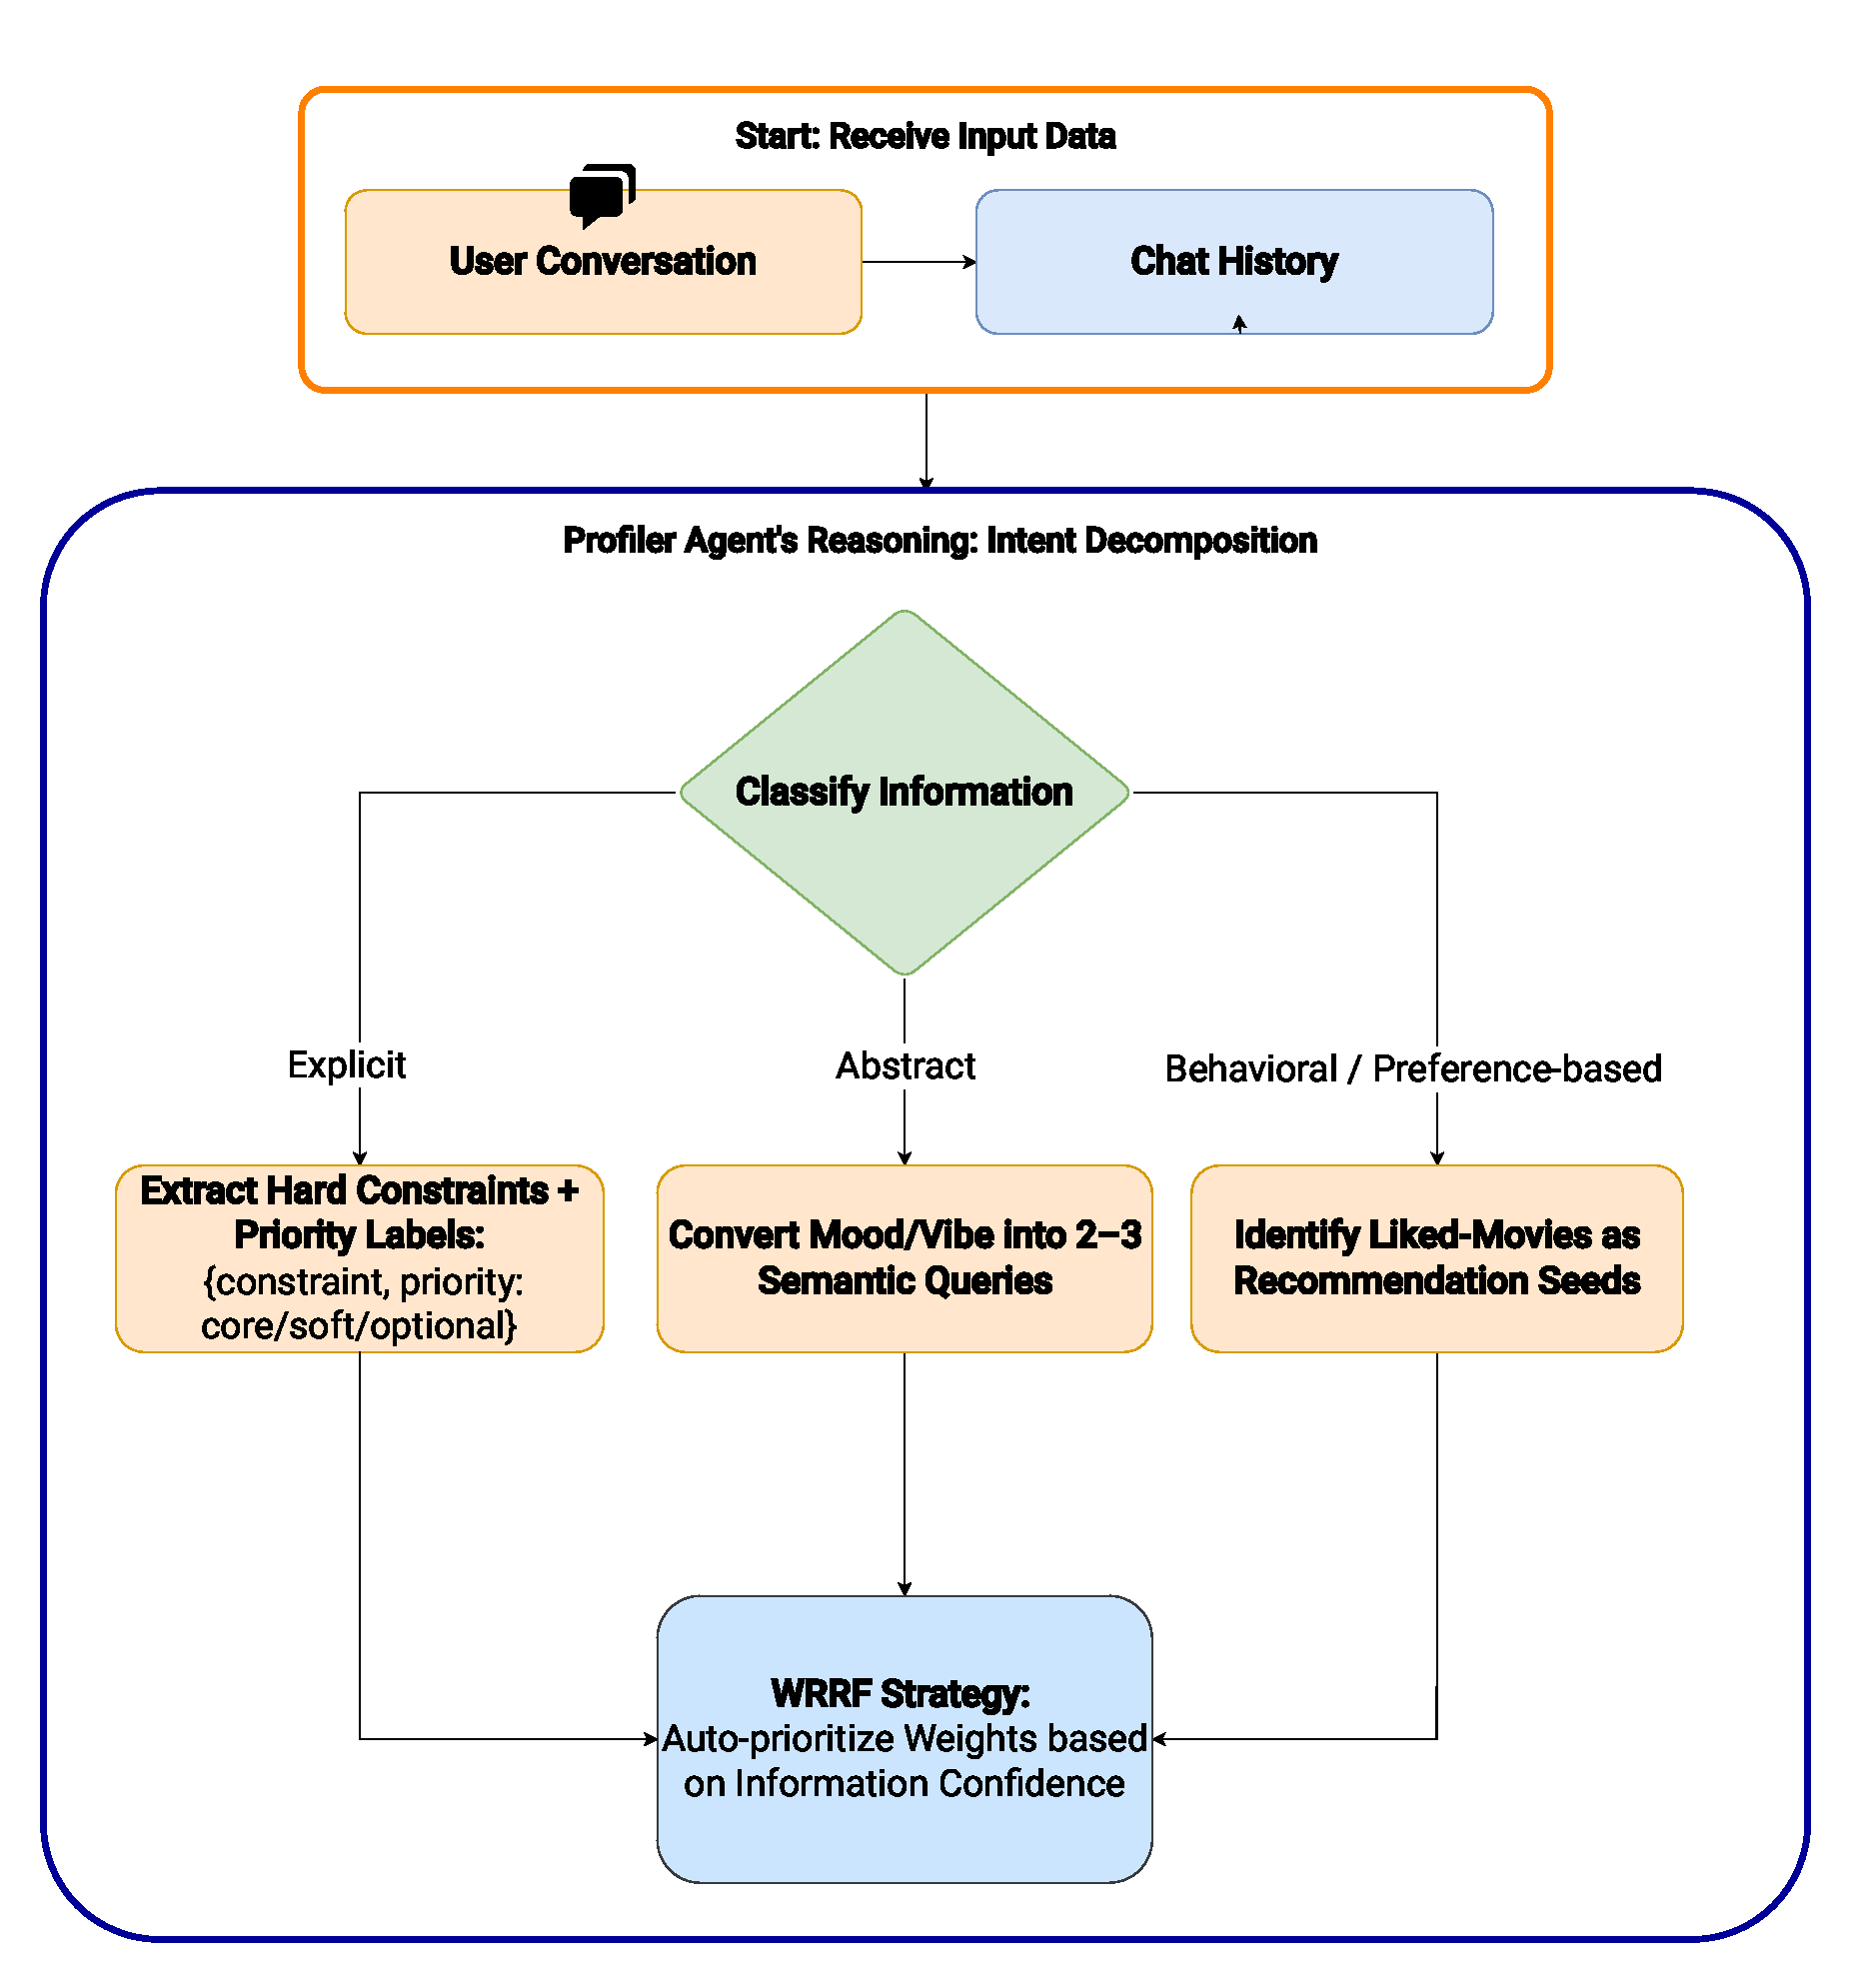
\includegraphics[width=\linewidth]{Chap4/images/profile_agent.pdf}
    \caption{Tổng quan luồng suy luận của Profiler Agent (Intent Decomposition). Từ đầu vào là lượt hội thoại hiện tại và lịch sử chat, tác tử phân loại thông tin thành ba nhánh xử lý độc lập: (1) thông tin \textit{Explicit} được trích xuất thành Ràng buộc cứng (năm, hãng phim, diễn viên); (2) thông tin \textit{Abstract} (cảm xúc, không khí) được chuyển đổi thành 2–3 câu truy vấn ngữ nghĩa; (3) thông tin \textit{Behavioral} (phim đã thích) được xác định làm hạt giống gợi ý (Recommendation Seeds). Ba nhánh hội tụ về bước chiến lược WRRF, nơi trọng số các luồng truy xuất được tự động ưu tiên theo độ tin cậy của từng loại thông tin.}
    \label{fig:profiler_agent}
\end{figure}

Như minh họa trong Hình \ref{fig:profiler_agent}, điểm cốt lõi của Profiler Agent nằm ở bước \textbf{Phân loại thông tin (Classify Information)}: thay vì xử lý đồng nhất toàn bộ phát ngôn người dùng, tác tử nhận diện \textit{bản chất} của từng mảnh thông tin và định tuyến sang pipeline phù hợp. Thông tin tường minh (Explicit) như tên diễn viên, năm phát hành hay hãng sản xuất đi thẳng vào tập Ràng buộc cứng để làm bộ lọc cho Critic Agent ở giai đoạn sau. Thông tin trừu tượng (Abstract) mang tính cảm xúc như "phim buồn" hay "không khí u ám" được diễn giải thành 2–3 câu truy vấn ngữ nghĩa độc lập nhằm khai thác tối đa không gian vector. Thông tin hành vi (Behavioral) — các bộ phim người dùng đã xem và yêu thích — được dùng làm hạt giống cho luồng Collaborative Retrieval. Sau khi cả ba nhánh hoàn tất, Profiler Agent tổng hợp kết quả và xác định bộ trọng số WRRF phù hợp nhất với hình thái truy vấn hiện tại, cung cấp tín hiệu định tuyến cho Orchestrator Agent.

\subsection{Trích xuất thực thể và Ràng buộc cứng (Fact Extraction)}

Nhiệm vụ trọng tâm của Profiler Agent trong giai đoạn này là chuyển hóa các phát ngôn ngôn ngữ tự nhiên vốn có tính đa nghĩa và mơ hồ thành một tập hợp các vị từ logic (logic predicates) xác định. Tác tử tiến hành nhận diện và trích xuất các thông tin định lượng (năm sản xuất, điểm đánh giá) hoặc các thực thể định danh (tên đạo diễn, diễn viên, hãng phim) có độ tin cậy cao từ ngữ cảnh hội thoại hiện tại và lịch sử tương tác.

Quá trình này không chỉ dừng lại ở việc nhận diện thực thể (Entity Recognition) mà còn bao gồm bước chuẩn hóa tri thức (Knowledge Normalization). Profiler Agent đối soát các thực thể thô được trích xuất với lược đồ hệ thống để đảm bảo tính đồng nhất. Các thông tin sau khi chuẩn hóa được hệ thống hóa thành bộ \textbf{Ràng buộc cứng (Hard Constraints)} theo một cấu trúc dữ liệu nghiêm ngặt. Việc sử dụng các mô hình xác thực dữ liệu đảm bảo rằng mọi đầu ra của LLM đều phải tuân thủ một lược đồ JSON (JSON Schema) tiền định, triệt tiêu các sai số về định dạng trong quá trình truyền tin giữa các tác tử. Một ví dụ về cấu trúc ràng buộc cứng được minh họa như sau:

\begin{verbatim}
{
  "genres": ["Action", "Sci-Fi"],
  "directors": ["Christopher Nolan"],
  "release_year_range": [2010, 2020],
  "forbidden_elements": ["Romance"],
  "min_rating": 8.0
}
\end{verbatim}

Điểm khác biệt quan trọng của ARGOS so với các hệ thống RAG thông thường nằm ở vai trò của bộ hồ sơ này. Các ràng buộc cứng đóng vai trò là tiêu chí kiểm định bắt buộc. Trong các khâu kiểm định hậu kỳ (Critic phase), bất kỳ vật phẩm gợi ý nào không thỏa mãn dù chỉ một tiêu chí trong danh sách trên (ví dụ: phim thuộc thể loại Romance dù người dùng đã cấm) sẽ bị loại bỏ ngay lập tức khỏi tập kết quả. Cơ chế này đóng vai trò như một bộ lọc tiền định, bảo vệ hệ thống khỏi các lỗi ảo giác ngữ nghĩa của mô hình ngôn ngữ ở các giai đoạn sau.

Song song với việc trích xuất ràng buộc cứng từ thông tin tường minh, Profiler Agent còn xử lý nhánh thứ ba trong sơ đồ phân loại: thông tin hành vi (Behavioral). Cụ thể, các bộ phim người dùng đã đề cập tích cực trong lịch sử hội thoại (ví dụ: \textit{"tôi rất thích John Wick"}) được nhận diện và đánh dấu là \textbf{hạt giống gợi ý (Recommendation Seeds)}. Tập hạt giống này được chuyển trực tiếp đến Orchestrator Agent để khởi động luồng Collaborative Retrieval — duyệt Đồ thị tri thức để tìm các phim có chung diễn viên, đạo diễn hoặc ekip sáng tạo với các hạt giống đó.


\subsection{Đa dạng hóa ngữ nghĩa (Intent Expansion / Multi-Query)}
Trong các mô hình truy xuất ngữ nghĩa (Dense Retrieval) truyền thống, việc mã hóa toàn bộ truy vấn phức tạp của người dùng vào một vector duy nhất (single embedding vector) thường dẫn đến hiện tượng "sụp đổ ngữ nghĩa" (semantic collapse). Khi một câu lệnh chứa nhiều khái niệm trực giao (orthogonal concepts), không gian vector thường phải lấy trung bình (average out), làm phai nhòa các đặc trưng quan trọng.

Để khắc phục hạn chế này, Profiler Agent triển khai chiến lược \textbf{đa truy vấn (Multi-Query Expansion)}. Thay vì chỉ sử dụng một biểu diễn chung, tác tử phân rã ý định ban đầu thành một tập hợp các góc độ truy vấn độc lập $Q = \{q_1, q_2, \dots, q_n\}$. Các câu truy vấn này khai thác các đặc trưng tiềm ẩn (latent semantic features) riêng biệt như:
\begin{itemize}
    \item \textbf{Cốt truyện và Chủ đề (Plot \& Theme):} Trích xuất nội dung lõi của câu chuyện.
    \item \textbf{Không khí và Cảm xúc (Vibe \& Mood):} Trích xuất sắc thái cảm nhận mà người dùng mong muốn.
    \item \textbf{Bối cảnh và Kỹ thuật điện ảnh (Setting \& Cinematography):} Các yếu tố về hình ảnh, thời đại hoặc phong cách.
\end{itemize}
Điển hình, một yêu cầu phức tạp như "Tôi muốn xem một phim giống John Wick, bối cảnh Châu Á nhưng mang màu sắc buồn bã" sẽ không bị nén thành một vector hỗn độn. Thay vì đó, Profiler phân giải nó thành: $q_1 =$ "hành động nhịp độ cao, sát thủ", $q_2 =$ "bối cảnh Nhật Bản hoặc Hồng Kông", và $q_3 =$ "tâm lý nặng nề, kết cục bi thảm".

Quá trình này giúp mở rộng không gian tìm kiếm đa chiều (multi-dimensional search space), gia tăng đáng kể tỷ lệ bao phủ (Recall) của hệ thống. Cần lưu ý rằng, mặc dù việc phân rã ý định có vẻ giống một phép toán hợp (OR) tại bước truy xuất để tối ưu độ phủ, tính hội tụ và điều kiện giao (AND) của các yêu cầu vẫn được đảm bảo chặt chẽ ở các giai đoạn sau thông qua thuật toán hợp nhất thứ hạng (Fusion) và bước đối soát của Critic Agent.

\subsection{Dự báo chiến lược trọng số động (Dynamic Weighting / Adaptive Routing)}
Trong kiến trúc tĩnh GRACE, việc hợp nhất kết quả từ nhiều luồng dữ liệu (Semantic, Content, Graph) phụ thuộc vào một bộ siêu tham số (hyperparameters) tĩnh. Tuy nhiên, mỗi truy vấn lại yêu cầu một cấu hình khác nhau. Ví dụ, câu hỏi "Phim nào của Christopher Nolan đạo diễn?" mang đậm tính cấu trúc, trong khi câu "Phim nào khiến tôi phải suy ngẫm về nhân sinh?" lại mang đậm tính ngữ nghĩa.

Sau khi hoàn tất bước phân loại thông tin, Profiler Agent tổng hợp kết quả từ cả ba nhánh để xác định bộ trọng số WRRF phù hợp. Nguyên tắc cốt lõi là \textbf{ưu tiên trọng số theo độ tin cậy của thông tin (Information Confidence)}: nhánh nào trích xuất được nhiều thông tin chất lượng cao thì luồng truy xuất tương ứng được khuếch đại. Dựa trên đó, Profiler Agent dự báo một vector phân bố trọng số $\mathbf{w}(C)$ cho các luồng truy xuất theo ngữ cảnh hội thoại $C$:
\begin{equation}
    \mathbf{w}(C) = (w_{\text{sem}}, w_{\text{con}}, w_{\text{col}})^T, \quad \text{với} \quad \sum_{i \in \{\text{sem, con, col}\}} w_i = 1, \quad w_i \in [0, 1]
\end{equation}
Trong đó:
\begin{itemize}
    \item $w_{\text{sem}}$ (Trọng số Ngữ nghĩa - Semantic Weight): Tăng cao khi truy vấn chứa nhiều tính từ mô tả, cảm xúc, hoặc so sánh tương đồng ("giống phim A nhưng buồn hơn").
    \item $w_{\text{con}}$ (Trọng số Nội dung - Content Weight): Được ưu tiên khi người dùng chỉ định rõ các tiêu chí lọc cứng như thể loại, khoảng năm phát hành, hoặc ngưỡng điểm đánh giá (IMDb/Rating).
    \item $w_{\text{col}}$ (Trọng số Đồ thị - Graph Weight): Được kích hoạt khi truy vấn chỉ định rõ các thực thể danh định (Entities) như tên diễn viên, đạo diễn, hãng phim, hoặc khi cần khai thác lịch sử hồ sơ người dùng (User Profile) để mở rộng tìm kiếm.
\end{itemize}
Việc định tuyến linh hoạt (Adaptive Routing) này giúp ARGOS tự động điều phối tài nguyên tìm kiếm, tối ưu hóa sự kết hợp của nhiều nguồn tri thức mà không cần sự can thiệp thủ công của kỹ sư vào mã nguồn. Cơ chế này được minh họa cụ thể trong Hình \ref{fig:adaptive_weighting}.

\begin{figure}[H]
    \centering
    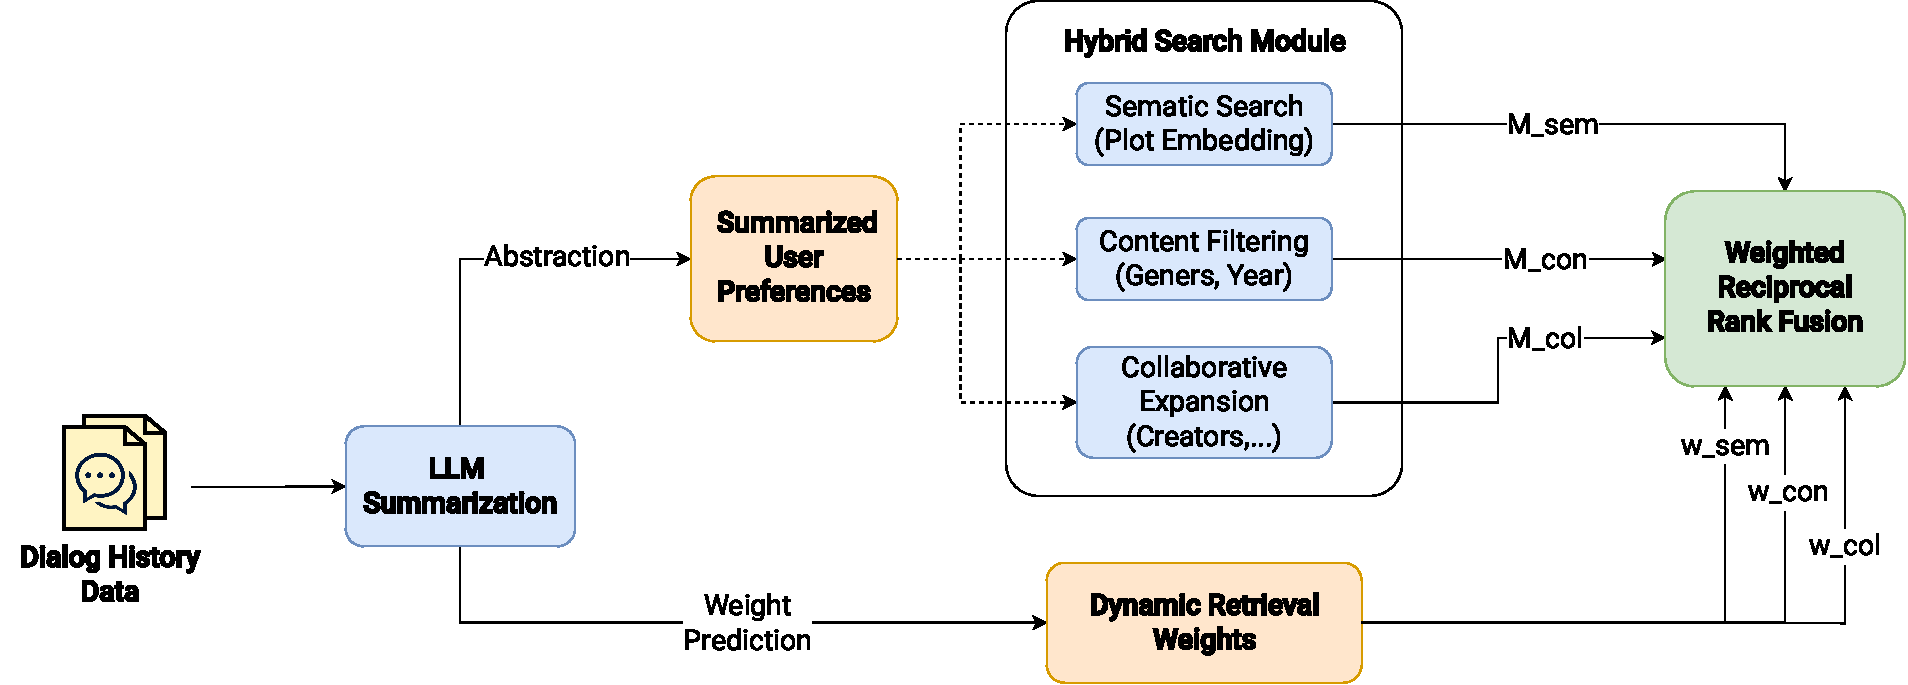
\includegraphics[width=\linewidth]{Chap4/images/adaptive_weighting.pdf}
    \caption{Cơ chế dự báo trọng số động (Dynamic Weight Prediction) do Profiler Agent thực hiện, cung cấp tín hiệu định tuyến cho các luồng truy xuất.}
    \label{fig:adaptive_weighting}
\end{figure}

\section{Tác tử Đồ thị (Graph Agent) với Vòng lặp ReAct}

Tác tử Đồ thị có nhiệm vụ tương tác trực tiếp với cơ sở dữ liệu đồ thị, khai thác cấu trúc đồ thị đa quan hệ (multi-relational graph structure) để định vị các thực thể thông qua các bước nhảy logic (multi-hop reasoning).

\subsection{Nhận thức cấu trúc dữ liệu (Schema-Aware Intelligence)}
Điểm yếu thường thấy khi giao tiếp tự do giữa LLM và cơ sở dữ liệu đồ thị là LLM có xu hướng "ảo giác" ra các nút (nodes) hoặc các mối quan hệ (edges) không hề tồn tại trong cơ sở dữ liệu thực tế. Ví dụ, LLM có thể sinh ra các câu truy vấn đồ thị sai lệch về cấu trúc nút, trong khi đồ thị thực tế chỉ cho phép những liên kết nhất định giữa các thực thể (như Người dùng thich Phim thay vì Người dùng thích Diễn viên). 

Để giải quyết vấn đề này, Graph Agent được trang bị cơ chế \textbf{Nhận thức cấu trúc dữ liệu (Schema-Aware Intelligence)}. Hệ thống liên tục cung cấp cho tác tử một siêu dữ liệu (metadata snapshot) chứa danh sách các nhãn (Labels) và các loại quan hệ (Relationships) hợp lệ. Nhờ sự ràng buộc khắt khe này, tác tử có thể ánh xạ chính xác các nhu cầu trừu tượng của người dùng vào không gian đồ thị. Đồng thời, tác tử được tích hợp khả năng khai thác các phương pháp truy vấn liên kết, cho phép đối chiếu danh sách các phim người dùng đã thích để nội suy các kết nối ẩn về diễn viên hoặc đạo diễn một cách an toàn.

\subsection{Vòng lặp Suy luận và Hành động (Reasoning + Acting)}
Đặc điểm cốt lõi tạo nên sự khác biệt của Graph Agent là việc tích hợp mô hình suy luận ReAct (Reasoning and Acting) \cite{yao2022react}. Khác với các hệ thống chuyển đổi ngôn ngữ sang truy vấn đồ thị (Text-to-Graph Query) thụ động, tác tử vận hành dựa trên một chuỗi các trạng thái động được định nghĩa hình thức tại bước $t$ như sau:
\begin{equation}
    \text{Thought}_t \rightarrow \text{Action}_t (\text{Graph Query}) \rightarrow \text{Observation}_t (\text{DB Result})
\end{equation}

Trong chu trình tối đa 3 lượt (turns), hệ thống tiến hành các bước:
\begin{enumerate}
    \item \textbf{Action:} Tác tử sinh mã truy vấn đồ thị dựa trên ý định đầu vào và sơ đồ cấu trúc.
    \item \textbf{Observation:} Khác biệt với các hệ thống tĩnh thường sụp đổ khi gặp lỗi biên dịch (compile error), Graph Agent thu nhận trực tiếp thông báo lỗi từ hệ quản trị cơ sở dữ liệu hoặc nhận về một danh sách kết quả rỗng (empty list).
    \item \textbf{Thought:} Dựa trên Observation, tác tử tự phân tích nguyên nhân sự cố. Nó nhận thức được rằng trường dữ liệu \texttt{'studio'} bị thiếu và tự động đề xuất giải pháp thay thế, chẳng hạn như chuyển sang tìm kiếm dựa trên \texttt{'production\_company'}.
\end{enumerate}
Cơ chế tự sửa lỗi (Self-Correction) này giúp hệ thống xử lý được các tình huống sai lệch cấu trúc đồ thị (Schema Mismatch) mà không cần lập trình viên viết thêm logic xử lý ngoại lệ cho từng trường hợp cụ thể. Quy trình này được mô phỏng chi tiết trong Hình \ref{fig:graph_agent_react}.


\begin{figure}[H]
    \centering
    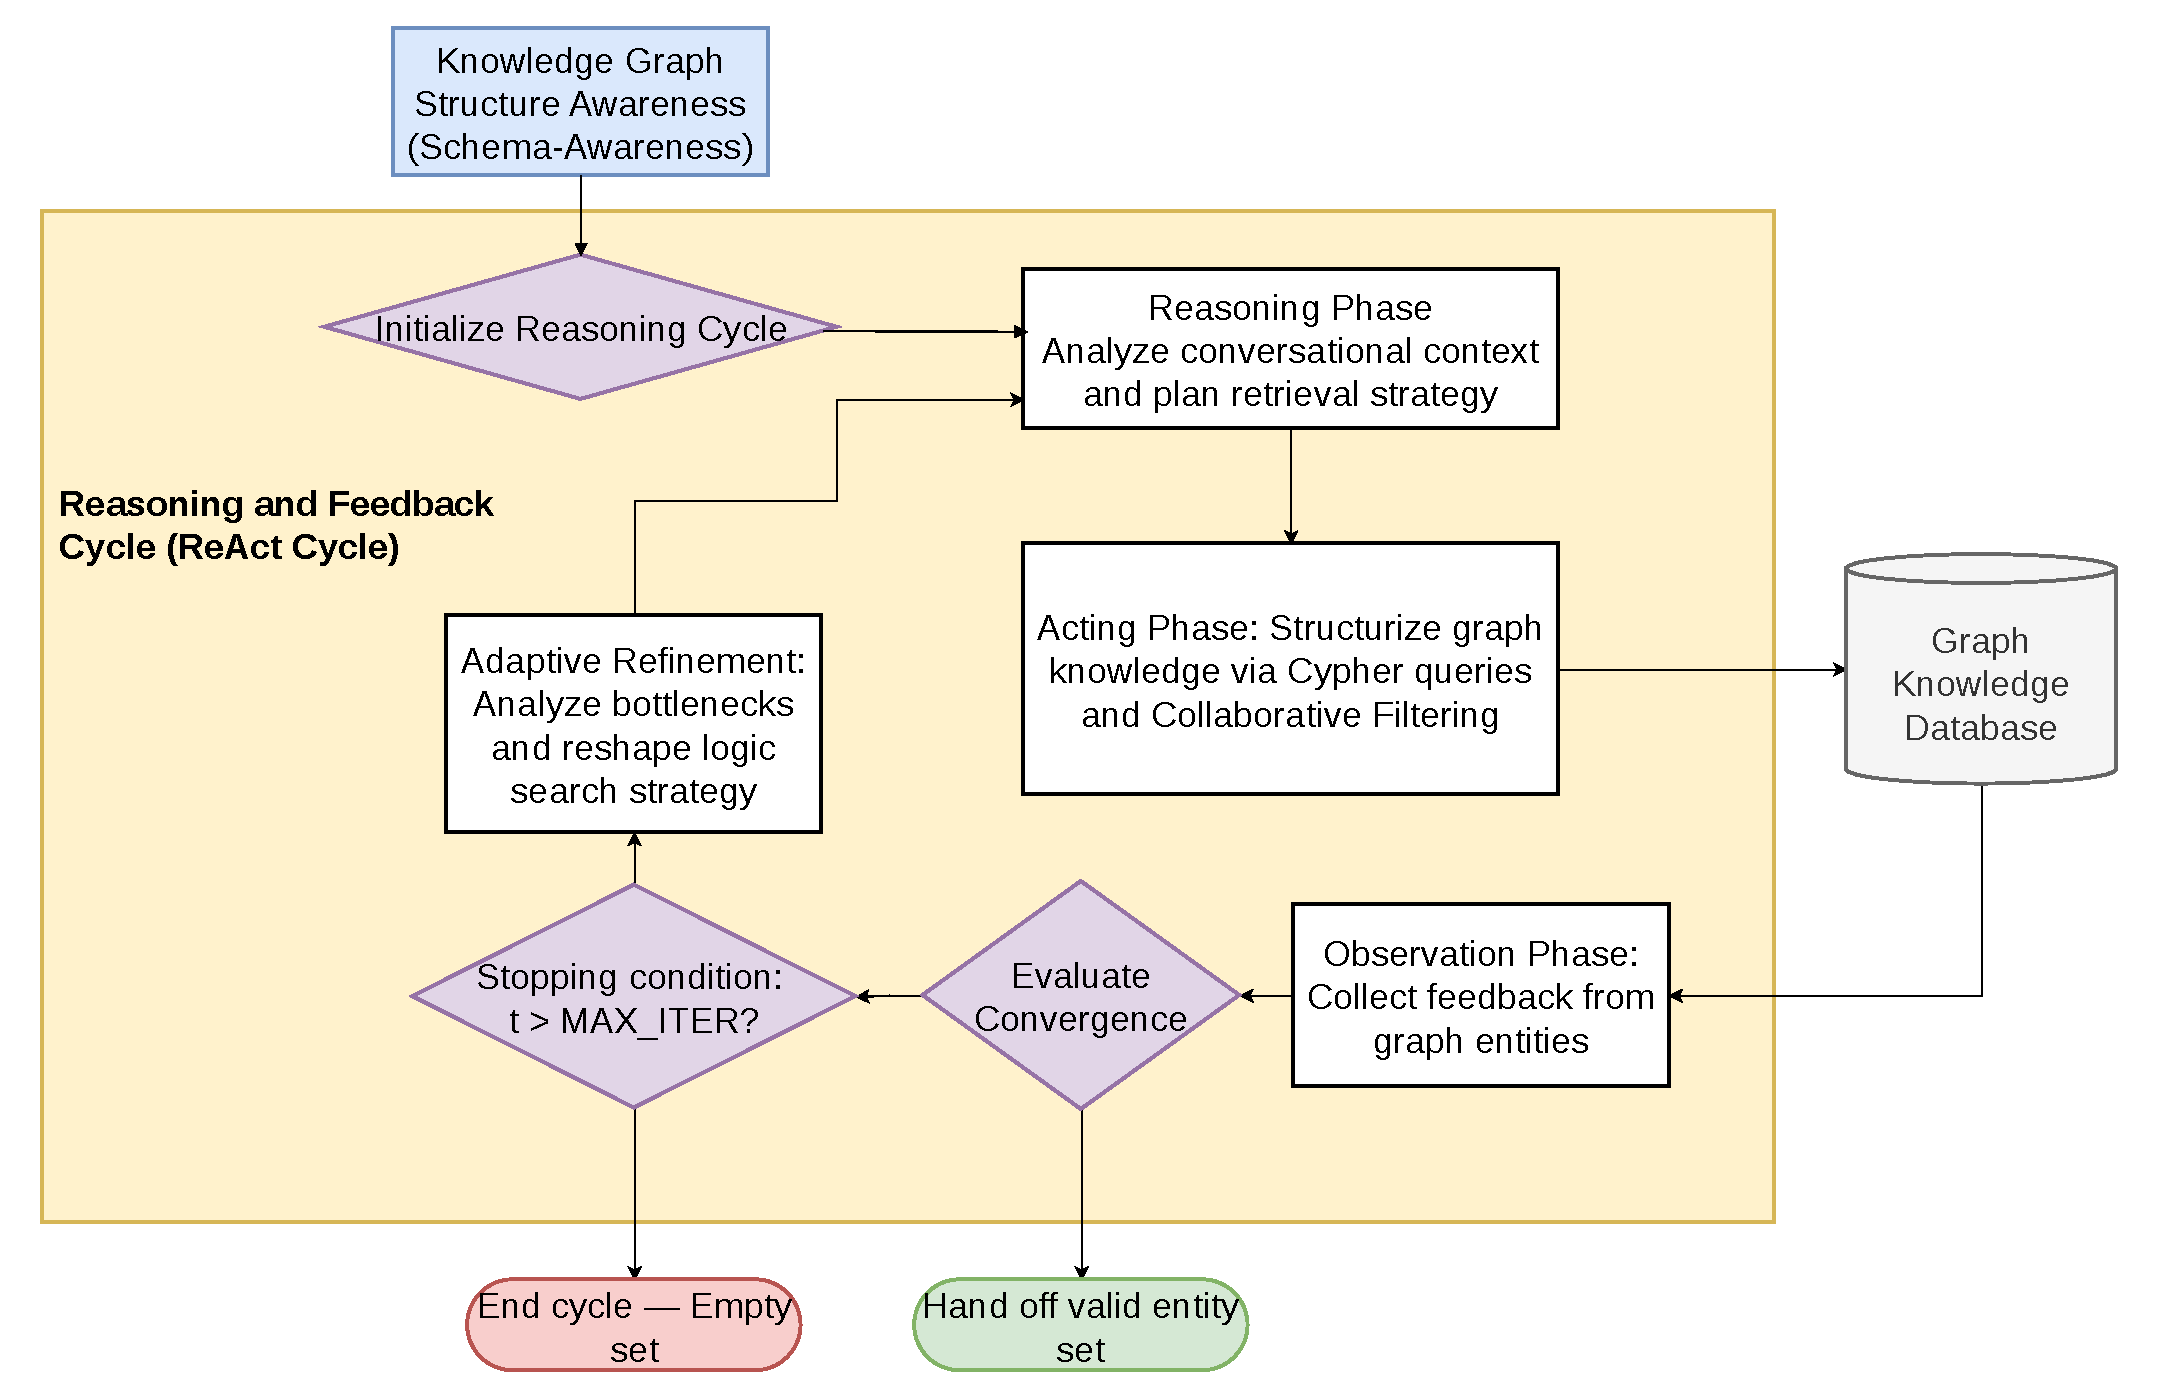
\includegraphics[width=\linewidth]{Chap4/images/graph_agent.pdf}
    \caption{Sơ đồ chu trình suy luận và phản hồi (ReAct Cycle) của Graph Agent. Dựa trên nhận thức về cấu trúc đồ thị (Schema-Awareness), hệ thống tiến hành vòng lặp Suy luận - Hành động - Quan sát, kết hợp cơ chế đánh giá tính hội tụ và tự thích nghi (Refinement) để tối ưu chiến lược truy vấn.}
    \label{fig:graph_agent_react}
\end{figure}

\section{Trung tâm Điều phối (Orchestrator Agent)}

Orchestrator Agent hoạt động như một module điều phối trung tâm, chịu trách nhiệm quản lý tài nguyên và tổng hợp thứ hạng. Hình \ref{fig:orchestrator_strategy} minh họa luồng tư duy và chiến lược tìm kiếm đa luồng của Orchestrator.

\begin{figure}[H]
    \centering
    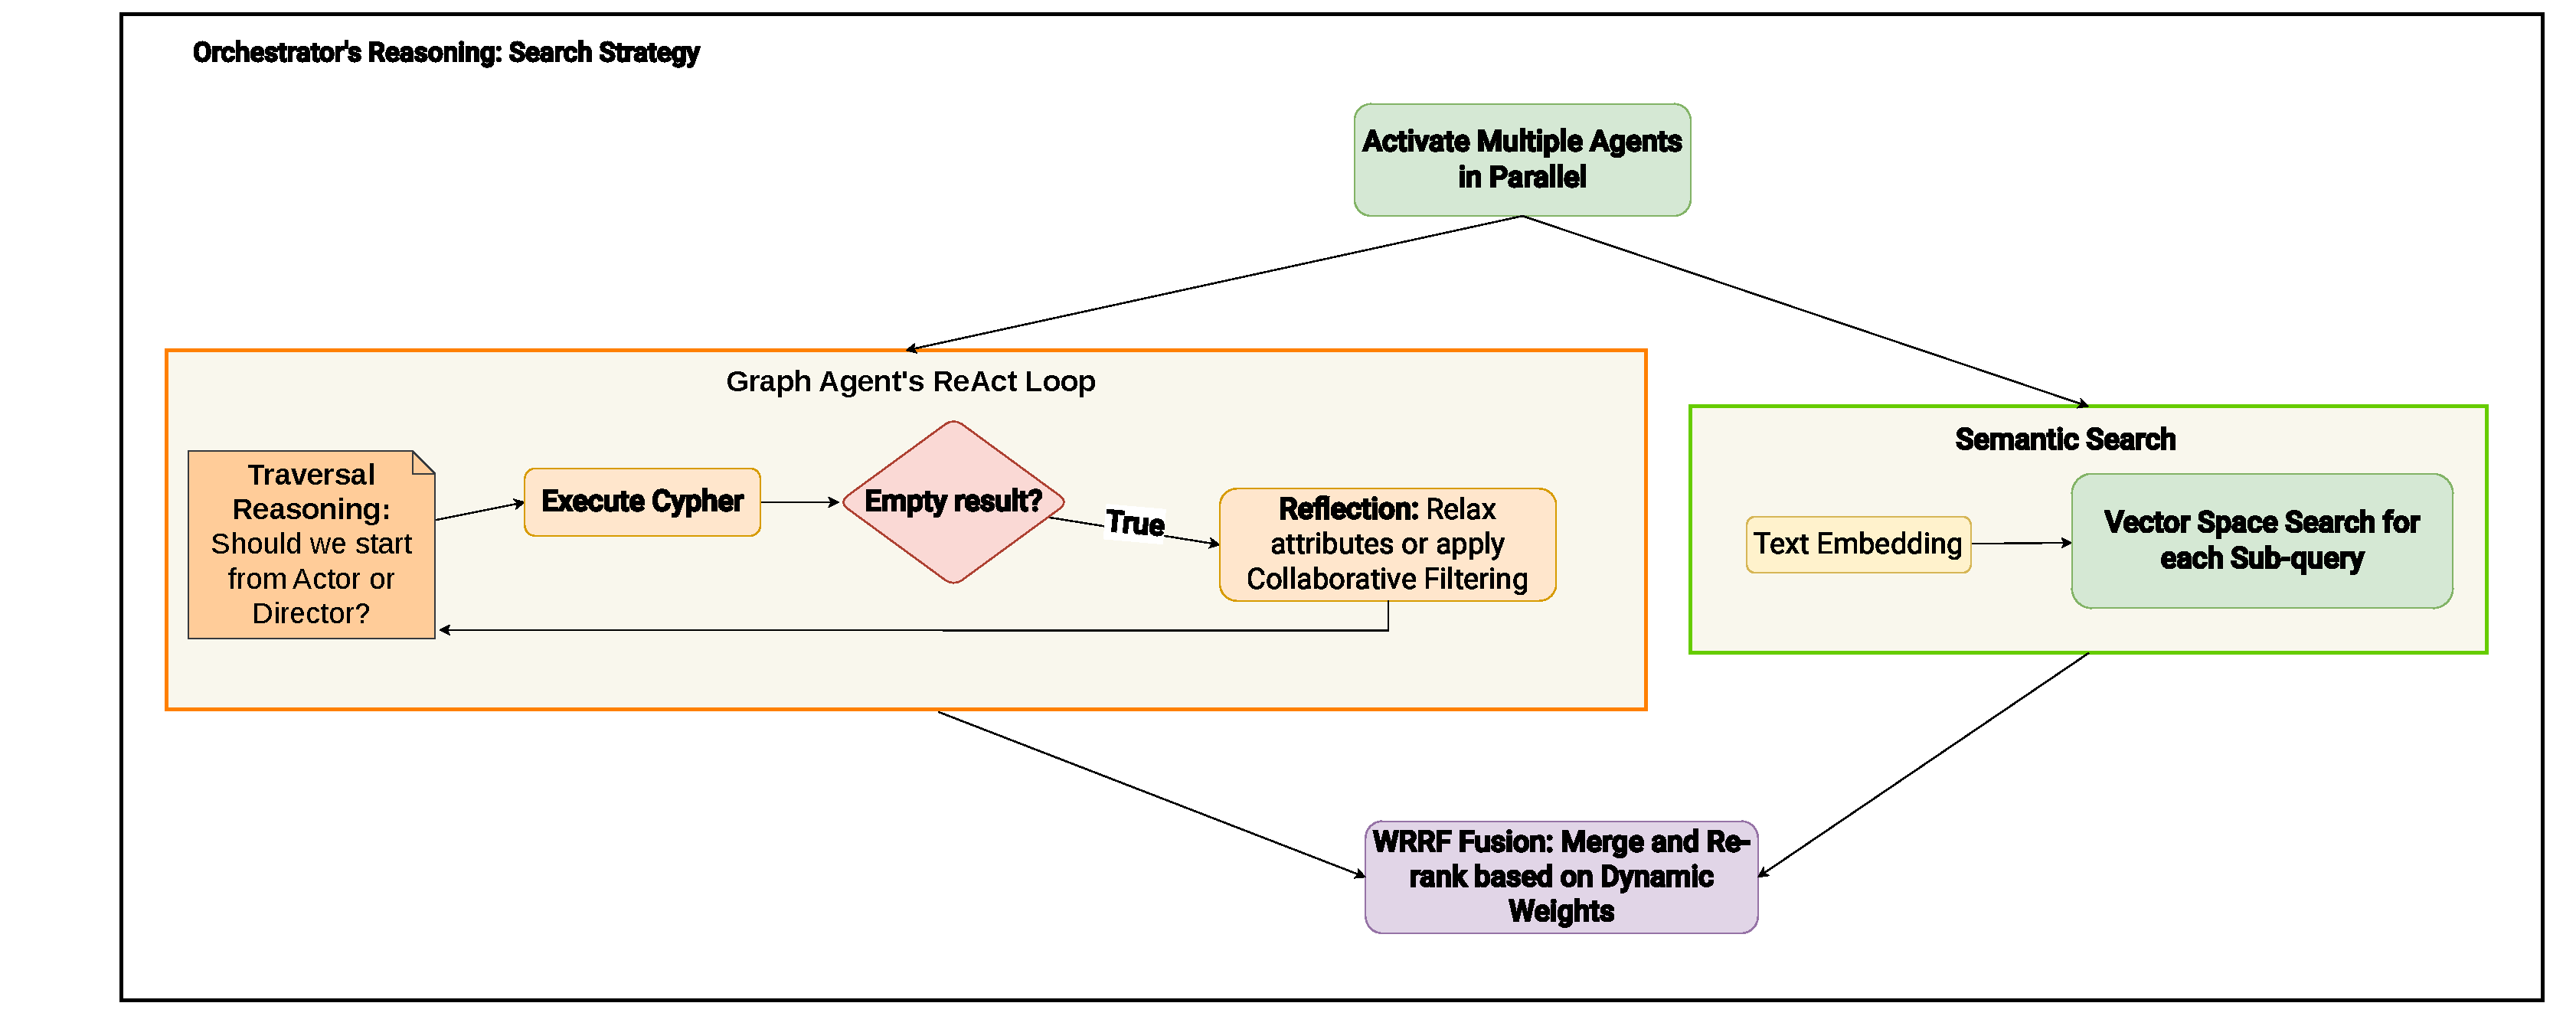
\includegraphics[width=\linewidth]{Chap4/images/Orchestrator.pdf}
    \caption{Chiến lược tìm kiếm đa luồng của Orchestrator Agent. Hệ thống kích hoạt song song Vòng lặp ReAct của Graph Agent và Tìm kiếm Ngữ nghĩa (Semantic Search), sau đó hợp nhất kết quả thông qua thuật toán WRRF Fusion có sử dụng trọng số động.}
    \label{fig:orchestrator_strategy}
\end{figure}

\subsection{Thực thi truy xuất bất đồng bộ (Asynchronous Parallel Execution)}
Khác với mô hình đường ống tuần tự (sequential pipeline), Orchestrator được thiết kế để tối thiểu hóa độ trễ (latency) thông qua kiến trúc lập trình bất đồng bộ (asynchronous programming). Ngay khi Profiler Agent hoàn tất việc phân rã ý định, Orchestrator sẽ kích hoạt đồng thời ba luồng truy xuất độc lập:
\begin{itemize}
    \item \textbf{Semantic Retrieval:} Tìm kiếm trên không gian vector mật độ cao (Dense Vector DB) để nắm bắt ý nghĩa tiềm ẩn.
    \item \textbf{Content Retrieval:} Khớp lệnh chính xác (Exact Match) trên cơ sở dữ liệu quan hệ hoặc hệ thống tìm kiếm văn bản để lọc theo các siêu dữ liệu cứng (metadata).
    \item \textbf{Graph Retrieval:} Thực thi vòng lặp ReAct của Graph Agent trên cơ sở dữ liệu đồ thị để tìm kiếm các thực thể liên kết đa bước.
\end{itemize}
Quá trình xử lý song song này đảm bảo hệ thống có thể quét qua toàn bộ mặt phẳng dữ liệu khổng lồ mà không làm tăng thời gian phản hồi tổng thể (Time-To-First-Token). Điểm nghẽn về tốc độ sẽ chỉ phụ thuộc vào luồng phản hồi chậm nhất (thường là Graph Agent), thay vì tổng thời gian của cả ba luồng cộng lại.

\subsection{Hợp nhất thứ hạng với thuật toán WRRF (Dynamic WRRF)}
Mỗi luồng truy xuất sẽ trả về một danh sách các ứng viên độc lập với thang điểm (score scale) hoàn toàn khác nhau (ví dụ: điểm Cosine Similarity của cơ sở dữ liệu Vector khác biệt hoàn toàn với điểm số cấu trúc của đồ thị). Để đồng bộ hóa, Orchestrator áp dụng thuật toán Hợp nhất Thứ hạng Nghịch đảo có Trọng số (Weighted Reciprocal Rank Fusion - WRRF).

Cho $R_m(i)$ là thứ hạng của vật phẩm $i$ trong danh sách trả về của phương pháp truy xuất $m \in \{\text{sem, con, col}\}$, điểm số cuối cùng của vật phẩm $i$ được tính bằng:
\begin{equation}
    \text{WRRF\_Score}(i) = \sum_{m} \frac{w_m}{k + R_m(i)}
\end{equation}
Trong đó:
\begin{itemize}
    \item $w_m$ là trọng số của phương pháp $m$ do Profiler Agent dự báo theo ngữ cảnh hội thoại tại mỗi lượt. Đây là khác biệt cốt lõi so với GRACE, nơi bộ trọng số được cố định tại $(w_{\text{sem}}, w_{\text{con}}, w_{\text{col}}) = (0.40, 0.35, 0.25)$ cho toàn bộ hệ thống.
    \item $k$ là một hằng số làm mượt (smoothing constant), thường được đặt bằng 60 để ngăn chặn các vật phẩm ở top 1 chiếm ưu thế quá mức.
\end{itemize}
Cơ chế WRRF vinh danh các ứng viên xuất hiện ở phần giao tập hợp (intersection) của nhiều phương pháp tìm kiếm (nghĩa là vừa có ngữ nghĩa tốt, vừa có liên kết đồ thị mạnh). Điều này giải quyết bài toán "điều kiện hợp" (OR) của Multi-Query: một vật phẩm chỉ thỏa mãn $q_1$ sẽ có thứ hạng thấp hơn nhiều so với vật phẩm thỏa mãn đồng thời cả $\{q_1, q_2, q_3\}$. Do đó, WRRF đóng vai trò như một phép toán "giao mềm" (soft AND), định hướng sự hội tụ về phía các kết quả thỏa mãn toàn diện ý định người dùng. Việc áp dụng trọng số động $w_m$ giúp khuếch đại ảnh hưởng của luồng dữ liệu phù hợp nhất với loại truy vấn, từ đó tạo ra một danh sách ứng viên ưu tú mang tính thích ứng cao để chuyển giao cho pha kiểm định.

\section{Tác tử Kiểm định (Critic Agent) - Kiểm soát chất lượng}

Tác tử kiểm định (Critic Agent) đóng vai trò là một cơ chế rà soát độc lập (Quality Gate) trong kiến trúc ARGOS, hoạt động như một đối trọng để kiểm soát tính hợp lệ của danh sách ứng viên do các module truy xuất cung cấp. Cơ chế hoạt động của Critic Agent được minh họa trong Hình \ref{fig:critic_agent}.


\begin{figure}[H]
    \centering
    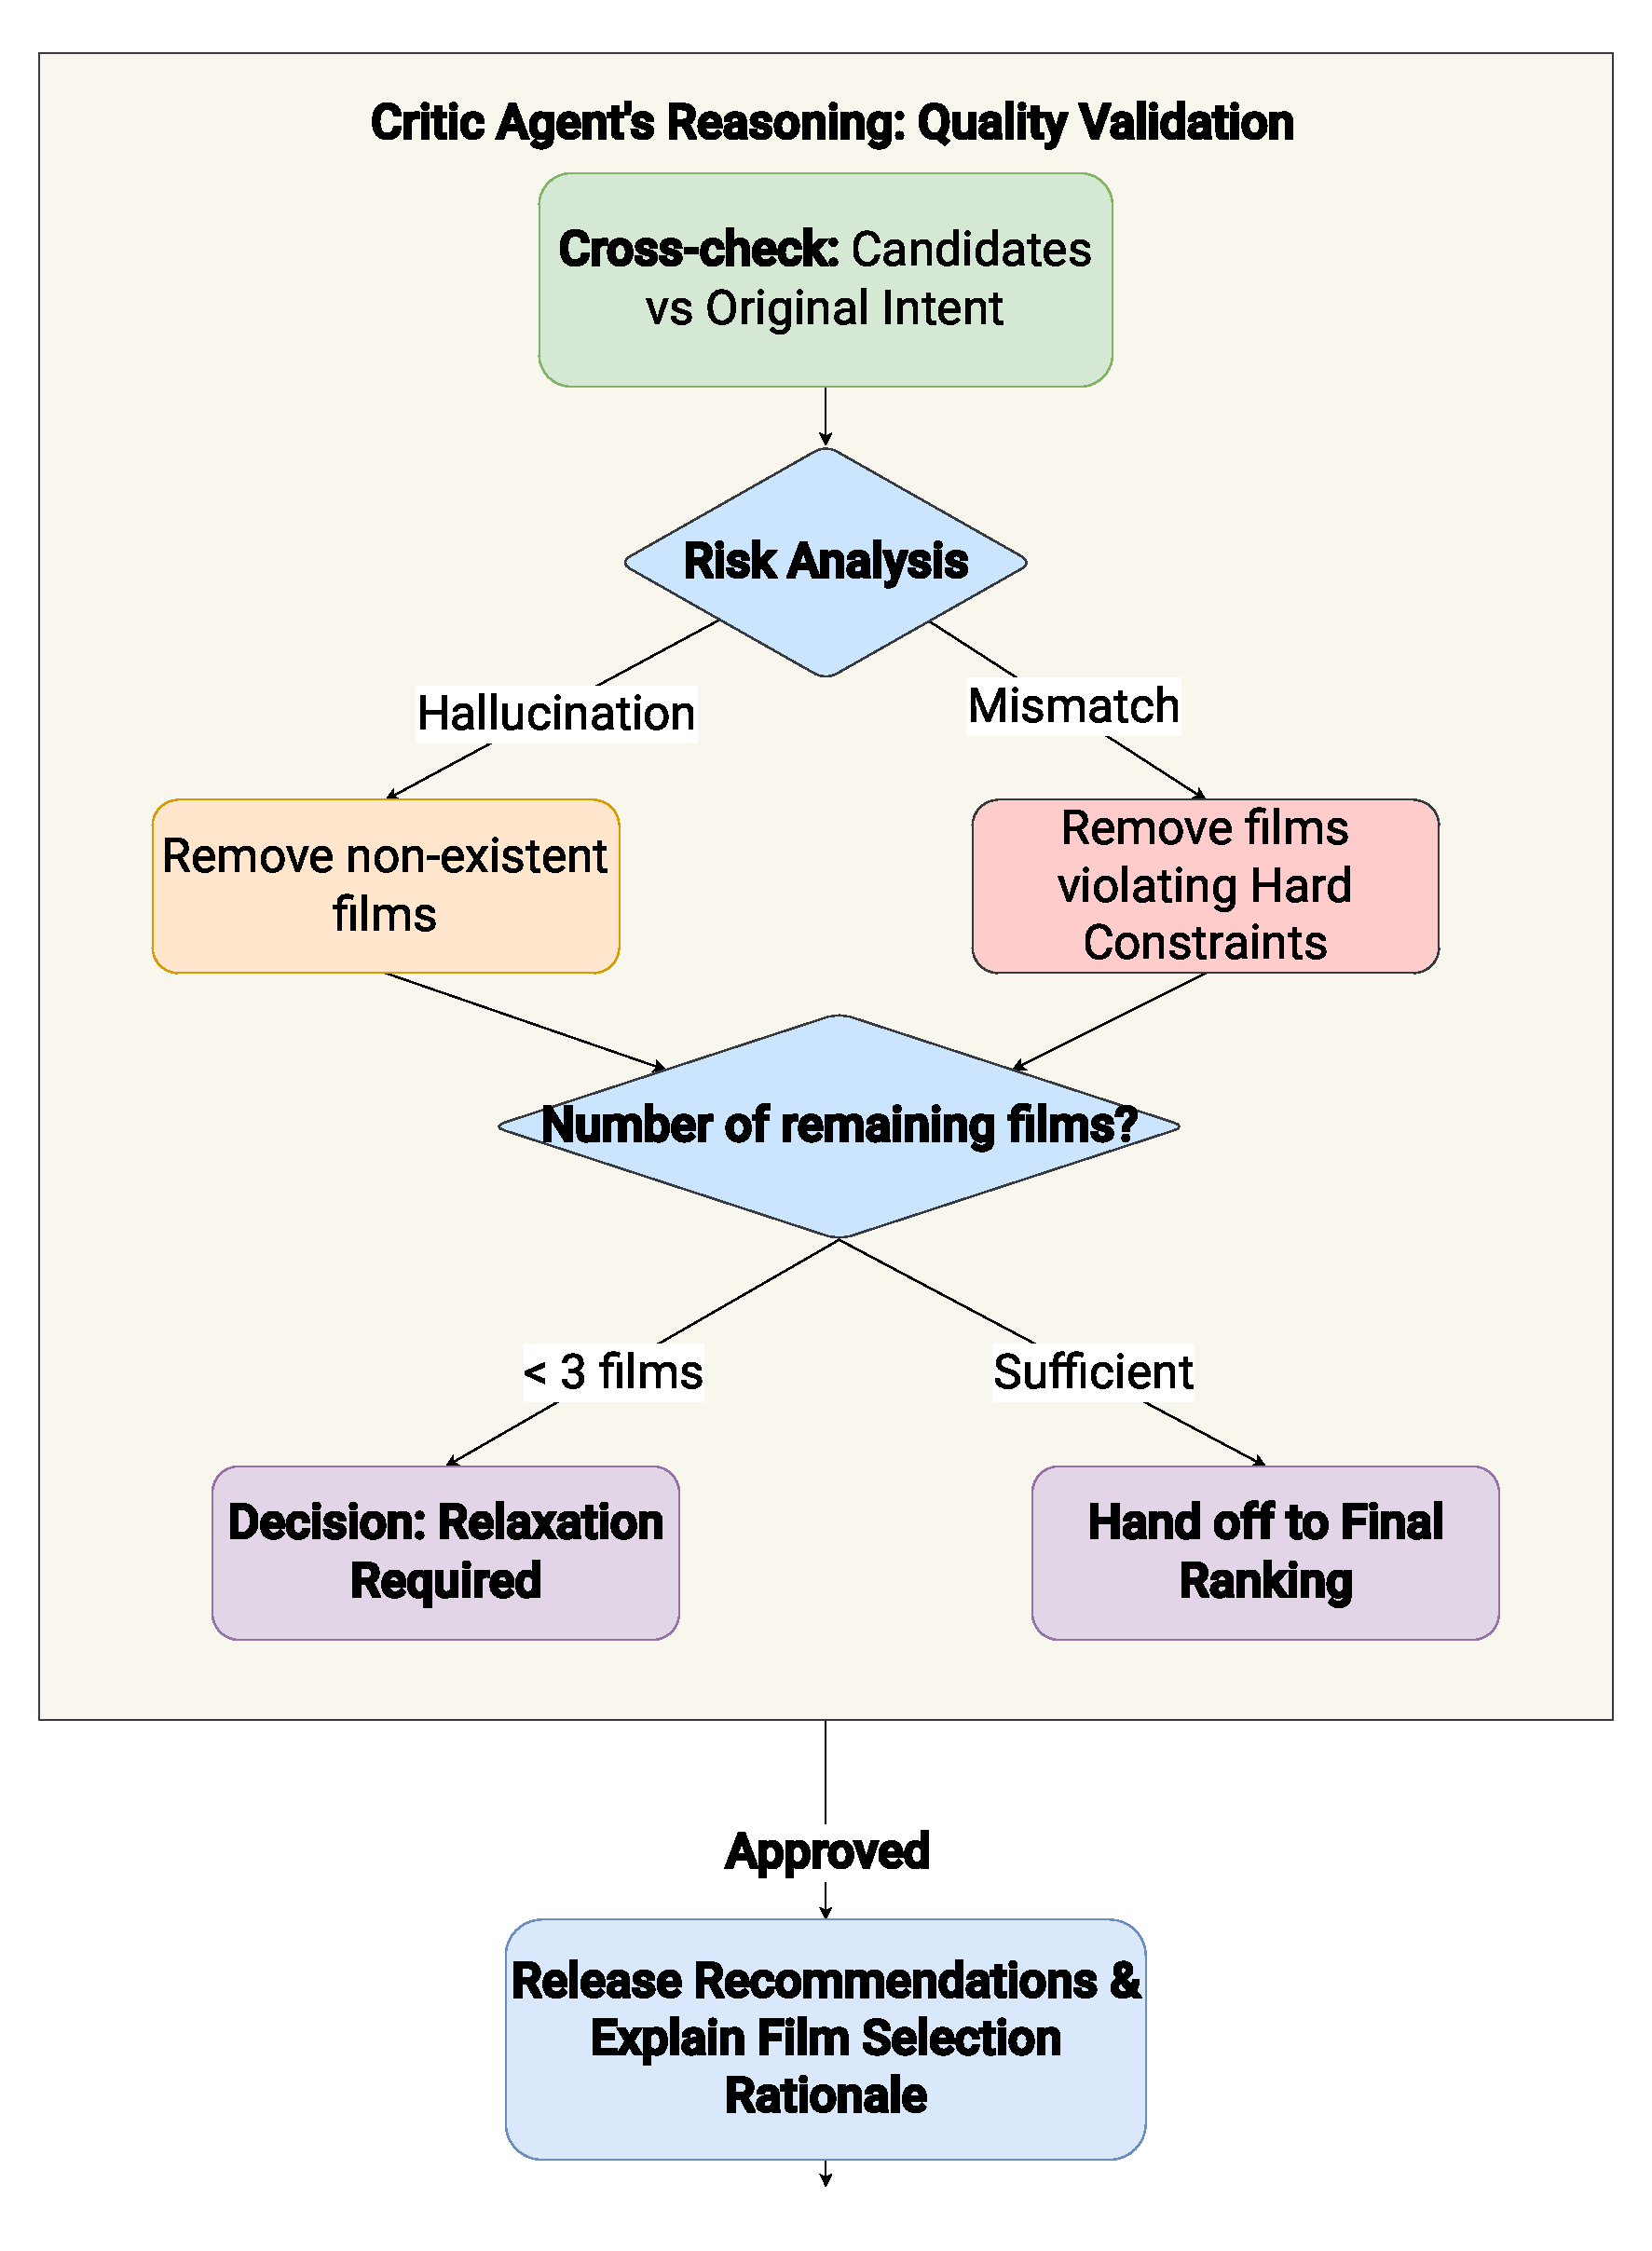
\includegraphics[width=\linewidth]{Chap4/images/critic_agent.pdf}
    \caption{Cơ chế hoạt động của Critic Agent. Tác tử thực hiện đối soát chéo các ứng viên với Ràng buộc cứng (Hard Constraints) và kích hoạt cơ chế phản hồi (Feedback Trigger) nếu số lượng ứng viên hợp lệ không đạt ngưỡng dung sai.}
    \label{fig:critic_agent}
\end{figure}

\subsection{Đối soát chéo và triệt tiêu ảo giác (Anti-Hallucination)}
Trong hệ thống RAG tĩnh, nếu LLM tự "bịa" ra một bộ phim không tồn tại (Fact Confabulation) hoặc đưa ra một phim không khớp với ràng buộc thời gian (Temporal Inconsistency), hệ thống thường chấp nhận và trả về trực tiếp cho người dùng. Điều này làm suy giảm nghiêm trọng độ tin cậy.

Danh sách ứng viên thu thập được từ Orchestrator sẽ trải qua quá trình đối soát nghiêm ngặt bởi Critic Agent. Tác tử thực hiện ánh xạ và so sánh trực tiếp các thuộc tính siêu dữ liệu (metadata) thực tế của từng ứng viên với tập hợp Ràng buộc cứng (Hard Constraints) đã được trích xuất ở pha Profiler. Quá trình này áp dụng logic Boolean chặt chẽ:
\begin{itemize}
    \item \textbf{Xác thực thực thể (Entity Verification):} Kiểm tra xem ID phim có thực sự tồn tại trong cơ sở dữ liệu hay không, loại bỏ hoàn toàn các phim do LLM tưởng tượng ra.
    \item \textbf{Kiểm tra ràng buộc loại trừ (Exclusion Check):} Đảm bảo không có bộ phim nào chứa các nhãn (tags) nằm trong danh sách \texttt{forbidden\_elements}.
    \item \textbf{Đánh giá ngưỡng (Thresholding):} Lọc bỏ các phim có điểm đánh giá (rating) thấp hơn \texttt{min\_rating} do người dùng quy định.
\end{itemize}
Những thực thể vi phạm bất kỳ ràng buộc logic nào sẽ bị loại bỏ không khoan nhượng nhằm bảo toàn chỉ số độ chuẩn xác (Precision) tuyệt đối của hệ thống.

\subsection{Kích hoạt phản hồi và Lập báo cáo lỗi (Feedback Trigger \& Error Reporting)}
Sau khi sàng lọc qua bộ Ràng buộc cứng, hệ thống thu được tập hợp ứng viên hợp lệ $M_{\text{valid}}$. Critic Agent thực hiện kiểm tra điều kiện ngắt quãng dựa trên ngưỡng dung sai $\tau$ (thường thiết lập $\tau = 1$ để đảm bảo ít nhất luôn có 1 kết quả trả về):
\begin{equation}
    \text{Trigger} =
    \begin{cases}
        \text{Accept},               & \text{nếu } |M_{\text{valid}}| \ge \tau \\
        \text{Relaxation\_Required}, & \text{nếu } |M_{\text{valid}}| < \tau
    \end{cases}
\end{equation}

Nếu tín hiệu \texttt{Relaxation\_Required} được phát ra, thay vì chỉ trả về trạng thái thất bại tĩnh (như mã lỗi 404), Critic Agent sẽ đóng vai trò như một kỹ sư kiểm thử (QA Engineer). Nó sẽ tổng hợp một báo cáo phân tích lỗi (Error Report) bằng ngôn ngữ tự nhiên hoặc JSON, chỉ rõ \textit{chính xác ràng buộc nào đã bị vi phạm}. Ví dụ: \textit{"Tìm thấy 5 phim hành động của đạo diễn Nolan, nhưng không có phim nào phát hành sau năm 2020 như yêu cầu."} Báo cáo này là cơ sở dữ liệu đầu vào mang tính sống còn để chuyển giao quyền điều khiển cho pha thỏa hiệp kế tiếp, định hướng cho hệ thống biết cần phải sửa chữa ở đâu.

\section{Tác tử Thỏa hiệp (Relaxation Agent) - Cơ chế tự sửa lỗi}

Trong trường hợp hệ thống không tìm được kết quả hợp lệ do các điều kiện truy vấn quá khắt khe, Relaxation Agent sẽ được kích hoạt để thực thi cơ chế nới lỏng ràng buộc, qua đó duy trì tính liên tục của luồng hội thoại. Hình \ref{fig:relaxation_agent} mô tả quy trình phân tích và tái cấu trúc ý định của tác tử này.


\begin{figure}[H]
    \centering
    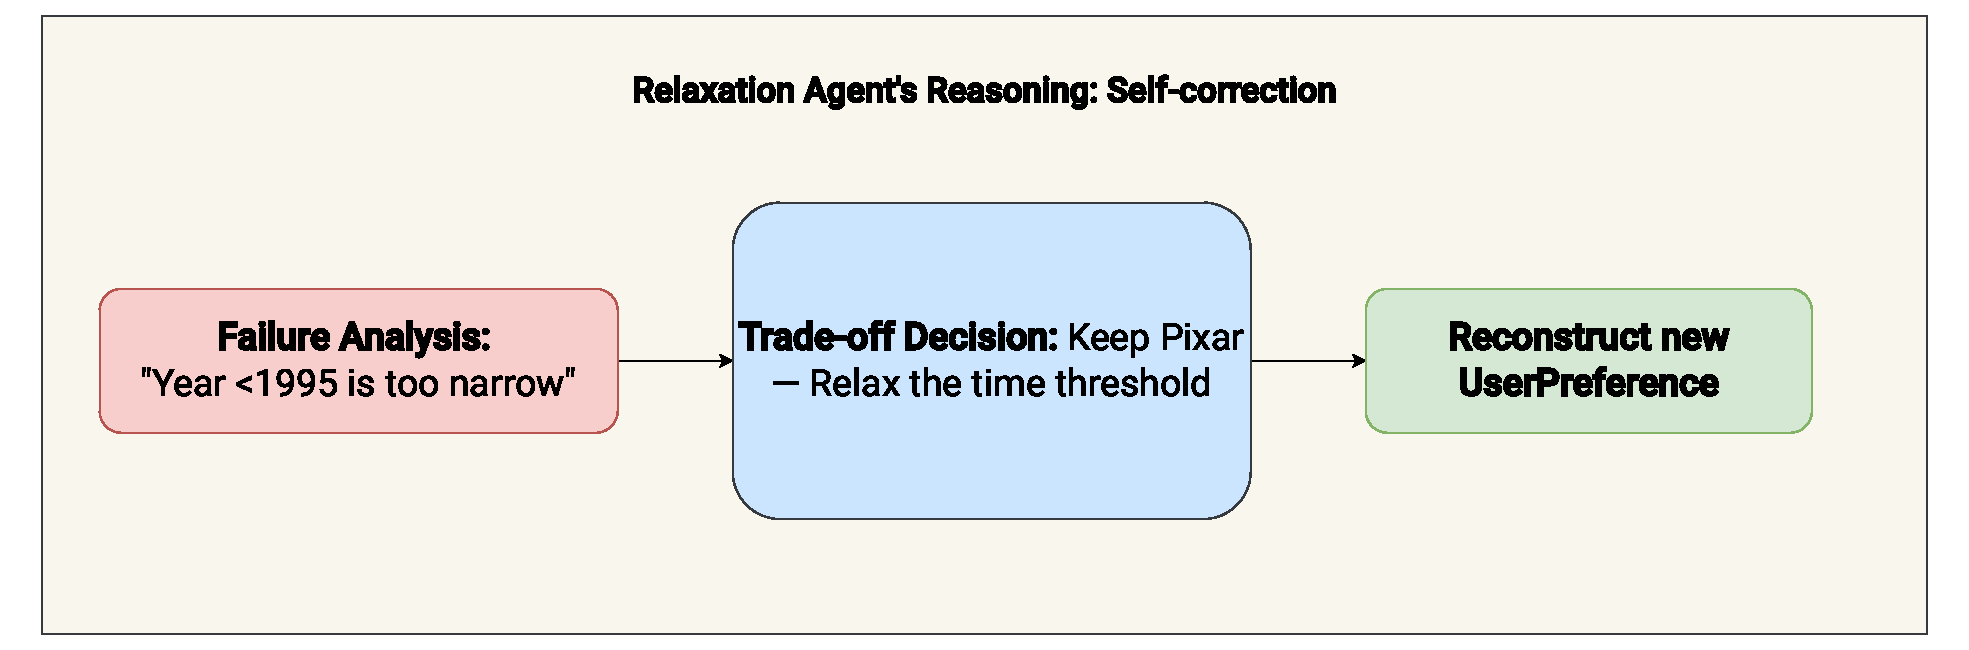
\includegraphics[width=\linewidth]{Chap4/images/relaxation_agent.pdf}
    \caption{Quy trình phân tích điểm nghẽn và tái cấu trúc ý định của Relaxation Agent. Dựa trên phân cấp ưu tiên (Sacrifice Hierarchy), tác tử nới lỏng các điều kiện tìm kiếm và khởi động lại vòng lặp hội thoại mới.}
    \label{fig:relaxation_agent}
\end{figure}

\subsection{Phân tích điểm nghẽn và Phân cấp ưu tiên (Sacrifice Hierarchy)}
Tác tử Thỏa hiệp tiếp nhận Báo cáo lỗi (Error Report) từ Critic Agent và tiến hành Phân tích điểm nghẽn (Bottleneck Analysis). Để hệ thống không rơi vào vòng lặp vô hạn (infinite loop) khi liên tục thử lại cùng một chiến lược thất bại, tác tử được trang bị một bộ nhớ trạng thái ngắn hạn (short-term state memory) để ghi nhận các ràng buộc đã từng được nới lỏng.

Cơ chế cốt lõi của bước này là việc xây dựng một cây \textbf{Phân cấp ưu tiên (Sacrifice Hierarchy)}. Tác tử sử dụng LLM để xác định các đặc trưng nào là "bất khả xâm phạm" (core properties) và đặc trưng nào mang tính thứ cấp (soft properties) dựa trên ngữ cảnh hội thoại. Ví dụ:
\begin{itemize}
    \item \textbf{Cốt lõi (Core):} Thể loại (Genre) thường là yếu tố quyết định. Nếu người dùng muốn xem "Phim Hài", hệ thống không được gợi ý "Phim Kinh dị".
    \item \textbf{Thứ cấp (Soft):} Niên đại phát hành (Release Year) hoặc điểm đánh giá (Rating) có thể được nới lỏng linh hoạt. Biên độ năm có thể được mở rộng từ $[2010, 2020]$ thành $[2005, 2025]$, hoặc hạ ngưỡng \texttt{min\_rating} từ $8.0$ xuống $7.5$.
\end{itemize}
Phương pháp thỏa hiệp tuần tự này dựa trên cơ sở tối ưu hóa hàm thỏa dụng dự kiến (expected utility) của người dùng, đảm bảo rằng kết quả trả về, dù không hoàn hảo 100\%, vẫn bám sát nhất có thể vào ý định gốc.

\subsection{Tái cấu trúc ý định (Intent Reconstruction)}
Sau khi thiết lập phương án thỏa hiệp dựa trên Sacrifice Hierarchy, Relaxation Agent tiến hành \textbf{Tái cấu trúc ý định (Intent Reconstruction)}. Quá trình này bao gồm hai thao tác:
\begin{enumerate}
    \item Khởi tạo lại cấu trúc hồ sơ sở thích (UserPreference JSON) với các ràng buộc đã được nới lỏng.
    \item Cập nhật lại danh sách truy vấn ngữ nghĩa (Multi-Queries) để phù hợp với hướng tiếp cận mới.
\end{enumerate}
Bản thiết kế mới này được đẩy ngược trở lại Orchestrator Agent, tự động kích hoạt vòng lặp tìm kiếm lần thứ hai (Attempt 2). Điểm đặc biệt của kiến trúc đa tác tử ARGOS là khả năng \textbf{tự phục hồi (self-healing)}. Khi kết quả cuối cùng được trả về cho người dùng, hệ thống luôn đính kèm một \textit{diễn giải logic phân nhánh (branching explanation)}, ví dụ: \textit{"Tôi không tìm thấy phim hoạt hình Pixar nào trước năm 1995, nhưng đây là một số tác phẩm xuất sắc của Studio Ghibli trong cùng thời kỳ"}. Cách diễn đạt này thừa nhận minh bạch giới hạn dữ liệu đồng thời vẫn mang lại gợi ý có giá trị, duy trì sự thông suốt của mạch hội thoại (Conversation Flow).

\section{Cải tiến Module Xếp hạng hai giai đoạn (Decoupled Reranking)}
GRACE sử dụng một Generative LLM duy nhất để xếp hạng toàn bộ danh sách ứng viên, hiệu quả nhưng chi phí tính toán tăng nhanh khi số ứng viên lớn. ARGOS cải tiến bằng cách phân tách thành hai giai đoạn, mỗi giai đoạn dùng mô hình phù hợp với yêu cầu tốc độ và độ sâu suy luận riêng biệt.

Sự cần thiết của phương pháp này xuất phát từ hai hạn chế cốt lõi của Generative LLM:
\begin{enumerate}
    \item \textbf{Hiện tượng Lost-in-the-Middle:} Khi đưa một danh sách dài hàng trăm ứng viên vào ngữ cảnh (context window) của LLM, mô hình thường chỉ tập trung vào các kết quả ở đầu và cuối văn bản, bỏ qua các thông tin quan trọng ở giữa.
    \item \textbf{Độ phức tạp tính toán (Computational Complexity):} Việc áp dụng cơ chế Self-Attention trên toàn bộ chuỗi văn bản của hàng trăm siêu dữ liệu phim sẽ dẫn đến phức tạp tính toán bậc hai ($O(N^2)$), tăng đáng kể chi phí API và độ trễ.
\end{enumerate}

Để giải quyết, quy trình Decoupled Reranking được thiết kế như sau:
\begin{itemize}
    \item \textbf{Giai đoạn 1 - Lọc nhanh với Cross-Encoder (SLM Reranker):} Ở giai đoạn này, hệ thống ứng dụng một mô hình ngôn ngữ quy mô nhỏ (Small Language Model - SLM) chuyên dụng cho tác vụ xếp hạng. Khác với Bi-Encoder (tìm kiếm vector) tính toán độc lập điểm số của truy vấn và tài liệu, Cross-Encoder nối trực tiếp truy vấn $q$ và tài liệu $d$ để đánh giá mức độ tương đồng ngữ nghĩa sâu: $\text{Score} = \text{SLM}(q \oplus d)$. Mô hình này đánh giá cực kỳ nhanh danh sách hàng trăm ứng viên thu được từ pha Orchestrator và chỉ giữ lại tập hợp $\text{Top-}20$ sắc bén nhất.
    \item \textbf{Giai đoạn 2 - Suy luận Logic với Generative LLM:} Danh sách $\text{Top-}20$ đã được tinh gọn sẽ được chuyển giao cho LLM cấu trúc lớn (Large Language Model) để thực hiện suy luận logic cuối cùng. Tại đây, LLM không chỉ đối sánh ngữ nghĩa mà còn cân nhắc tính đa dạng (Diversity), sự bất ngờ (Serendipity) và lịch sử hội thoại để chọn lọc ra $\text{Top-}5$ kết quả xuất sắc nhất trình bày cho người dùng.
\end{itemize}
Cải tiến này khai thác tối đa lợi thế tốc độ của mô hình truy xuất chuyên dụng (SLM) đồng thời bảo toàn năng lực biện luận bậc cao của mô hình sinh ngôn ngữ (LLM). Việc thiết lập $K_1 = 20$ và $K_2 = 5$ là điểm cân bằng giữa tỷ lệ bao phủ (Recall) và thời gian phản hồi, được xác nhận qua phân tích thực nghiệm tại Chương 5. Quy trình xếp hạng hai giai đoạn này được tổng quát hóa trong Hình \ref{fig:argos_reranker}.


\begin{figure}[H]
    \centering
    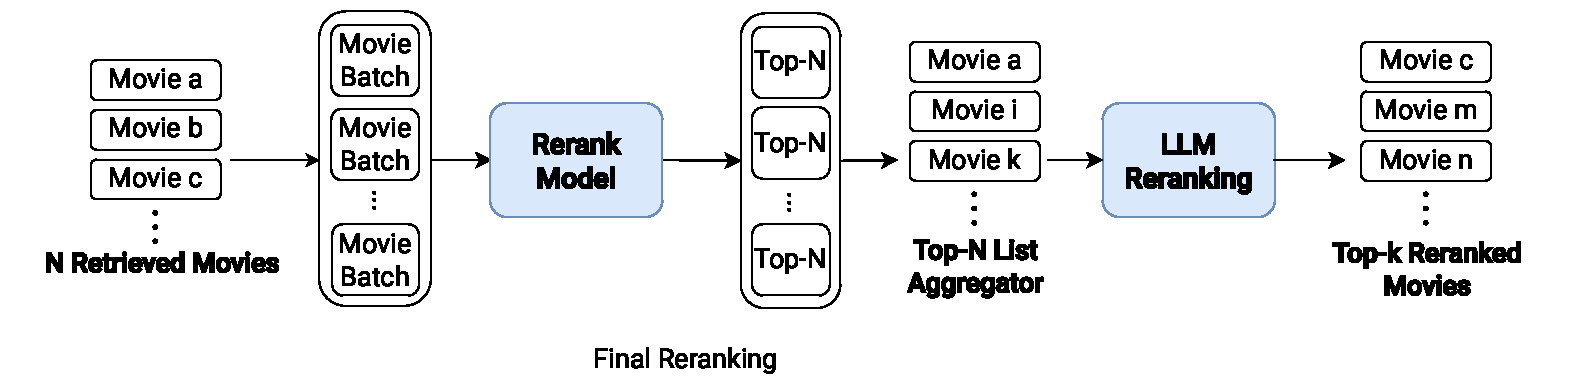
\includegraphics[width=\linewidth]{Chap4/images/Reranker.pdf}
    \caption{Quy trình xếp hạng hai giai đoạn (2-stage Reranking). Hệ thống kết hợp mô hình Rerank chuyên dụng để lọc nhanh danh sách ứng viên, sau đó tận dụng LLM để đánh giá sâu logic và đưa ra kết quả cuối cùng.}
    \label{fig:argos_reranker}
\end{figure}

\subsection{Sinh phản hồi hội thoại (Dialogue Response Generation)}
Sau khi Decoupled Reranking hoàn tất, danh sách $\text{Top-}5$ ứng viên cùng lịch sử hội thoại $C_t$ được chuyển giao cho Generative LLM để sinh phản hồi ngôn ngữ tự nhiên. Thay vì chỉ liệt kê tên phim, LLM tổng hợp lý do gợi ý từ các đặc trưng đã trích xuất (thể loại, đạo diễn, bầu không khí), tạo ra phản hồi cá nhân hóa và có thể giải thích được (Explainable Recommendation). Nếu Relaxation Agent đã nới lỏng một ràng buộc trong lượt truy xuất, thông tin về thỏa hiệp đó được đưa vào prompt để LLM sinh diễn giải phù hợp, ví dụ: \textit{"Không tìm thấy phim của Nolan phát hành sau 2020, nhưng đây là ba tác phẩm mang phong cách tương tự gần nhất."}\ Cơ chế này khép kín toàn bộ luồng xử lý của ARGOS từ ý định người dùng đến phản hồi hội thoại cuối cùng.

\section*{Kết luận chương}

Chương 4 đã trình bày chi tiết về thiết kế cấu trúc và luồng vận hành của hệ thống đa tác tử ARGOS. Bằng cách thay thế mô hình đường ống tĩnh một chiều, ARGOS xây dựng một quy trình cộng tác phân tán: bắt đầu từ khâu phân rã ý định và dự báo trọng số của \textit{Profiler Agent}, quá trình suy luận cấu trúc của \textit{Graph Agent}, khả năng điều phối của \textit{Orchestrator Agent}, cho đến các cơ chế kiểm soát chất lượng chặt chẽ của \textit{Critic Agent} và \textit{Relaxation Agent}. Cấu trúc này, khi kết hợp cùng phương pháp Xếp hạng hai giai đoạn (Decoupled Reranking), nhằm mục tiêu tối ưu hóa sự cân bằng giữa tính chính xác và độ trễ tính toán. Hiệu năng thực tiễn của kiến trúc này sẽ được định lượng và phân tích chi tiết thông qua các bài toán đánh giá thực nghiệm trong Chương 5.

% ----------------------CHƯƠNG 5----------------------
\chapter{Thiết lập và Kết quả Thực nghiệm}\label{chap:experiments}

Chương này trình bày chi tiết về quy trình thiết lập môi trường, các thước đo đánh giá và kết quả thực nghiệm của hệ thống ARGOS trên hai bộ dữ liệu ReDial và INSPIRED. Bên cạnh các phân tích định lượng nhằm so sánh hiệu năng với mô hình tiền đề GRACE và các hệ thống hiện đại (SOTA), chương này cung cấp các nghiên cứu tình huống (Case Studies) nhằm minh họa tính linh hoạt và khả năng xử lý suy luận của kiến trúc đa tác tử trong các kịch bản hội thoại thực tế.

\section{Thiết lập thí nghiệm}

\subsection{Tập dữ liệu ReDial và INSPIRED}
Hệ thống được đánh giá trên hai bộ dữ liệu chuẩn mực trong lĩnh vực Hệ thống gợi ý hội thoại (CRS):
\begin{itemize}
    \item \textbf{ReDial (Recommendation Dialogues) \cite{li2018towards}:} Chứa khoảng 10.000 đoạn hội thoại quy mô lớn, được sử dụng để đánh giá độ chính xác cốt lõi của khả năng truy xuất và sự phù hợp của các gợi ý.
    \item \textbf{INSPIRED \cite{hayati-etal-2020-inspired}:} Một tập dữ liệu chuyên biệt gồm 1.001 đoạn hội thoại, được thiết kế để kiểm tra khả năng duy trì mạch đối thoại tự nhiên, có chiến lược và mang tính xã hội cao của hệ thống.
\end{itemize}

\subsection{Cấu hình hệ thống và Phương pháp đánh giá}

Đồ thị tri thức được xây dựng trên Neo4j 5.15.0, sử dụng các phép toán \texttt{MERGE} lũy đẳng để đảm bảo không trùng lặp nút.

\textbf{Lựa chọn mô hình.}
\begin{itemize}
    \item \textbf{Gemini 2.0 Flash} (\texttt{temperature = 0.0}): Được dùng cho toàn bộ các tác vụ suy luận: Profiler Agent, Graph Agent, Critic Agent, Relaxation Agent và sinh phản hồi cuối. Nhiệt độ $0.0$ tối đa hóa tính xác định (determinism), giảm rủi ro hallucination trong môi trường yêu cầu đầu ra có cấu trúc JSON.
    \item \textbf{Cohere Rerank 4 Pro} (qua AWS Bedrock, model ID: \texttt{cohere.rerank-v3-5:0}): Cross-Encoder chuyên dụng cho Stage 1 của Decoupled Reranking, cho phép đánh giá tương đồng ngữ nghĩa sâu mà không cần tăng ngữ cảnh LLM.
    \item \textbf{\texttt{text-embedding-3-large}} ($d = 3072$): Mô hình nhúng vector của OpenAI, dùng cho Semantic Retrieval và xây dựng chỉ mục vector ChromaDB.
\end{itemize}

\textbf{Siêu tham số hệ thống.}
Bảng \ref{tab:hyperparams} tổng hợp các siêu tham số chính được cố định trong suốt quá trình thực nghiệm.

\begin{table}[H]
    \caption{Siêu tham số hệ thống ARGOS}
    \label{tab:hyperparams}
    \centering
    \begin{tabular}{lll}
        \toprule
        \textbf{Thành phần} & \textbf{Tham số} & \textbf{Giá trị} \\
        \midrule
        WRRF & Hằng số làm mượt $k$ & 60 \\
        WRRF & Trọng số mặc định $(w_{\text{sem}}, w_{\text{con}}, w_{\text{col}})$ & $(0.40,\ 0.30,\ 0.30)$ \\
        Orchestrator & Số ứng viên mỗi luồng $n$ & 20 \\
        Reranker Stage 1 & Kích thước batch $B$ & 100 \\
        Reranker Stage 1 & Shortlist mỗi batch $h$ & 20 \\
        Reranker Stage 2 & Kết quả cuối $K_2$ & 5 \\
        Graph Agent & Số lượt ReAct tối đa & 3 \\
        Critic Agent & Số ứng viên tối đa mỗi lần đánh giá & 50 \\
        Relaxation Agent & Số lần thử tối đa & 2 \\
        \bottomrule
    \end{tabular}
\end{table}

\textbf{Chiến lược lấy mẫu và kiểm định thống kê.}
Mô hình tiền đề GRACE được đánh giá trên toàn bộ (100\%) tập kiểm thử để thiết lập mốc tham chiếu chính xác khi so sánh với các mô hình SOTA đã công bố. Do giới hạn về tần suất gọi API và chi phí suy luận của hệ thống đa tác tử, ARGOS được đánh giá trên tập mẫu ngẫu nhiên đồng nhất gồm \textbf{20\%} dữ liệu kiểm thử (tương đương $\sim 925$ hội thoại trên ReDial). Kích thước mẫu này đảm bảo biên độ sai số dưới $\pm 3.0\%$ ở độ tin cậy 95\%. Kết quả được chia thành 5 tập con (5-fold cross-validation offline) để thực hiện kiểm định t-test, xác nhận các cải thiện đạt mức ý nghĩa thống kê ($p < 0.05$).

\textbf{Mã nguồn mở.}
Toàn bộ mã nguồn, kịch bản thực nghiệm và dữ liệu được công bố tại \url{https://github.com/DatPhan06/GRACE} để cộng đồng có thể kiểm chứng và tái lập kết quả.

\section{Kết quả đánh giá hệ thống}

\subsection{Khẳng định năng lực của kiến trúc tiền đề (GRACE vs. SOTA)}

Bảng \ref{tab:baseline_comparison} tóm tắt hiệu năng của kiến trúc tiền đề GRACE so với các hệ thống hiện đại (SOTA). Dữ liệu thực nghiệm cho thấy GRACE mang lại sự cải thiện toàn diện trên nhiều khía cạnh:

\textbf{So sánh với các Baseline CRS truyền thống:}
GRACE thể hiện sự vượt trội rõ rệt so với các mô hình dựa trên RNN hoặc mạng nơ-ron đồ thị sơ khai (như KGSF, CR-Walker, và KERL). Trong khi các hệ thống cũ bị giới hạn bởi khả năng hiểu ngôn ngữ tự nhiên kém và cách tích hợp đồ thị nông (shallow integration), luồng truy xuất lai (hybrid retrieval) của GRACE có khả năng nắm bắt các kết nối đa bước (multi-hop) phức tạp, dẫn đến độ phủ (Recall) cao hơn hẳn ở mọi ngưỡng cắt.

\textbf{So sánh với các Baseline dựa trên LLM (Prompting):}
Kiến trúc đề xuất cho thấy hiệu suất cao hơn so với cả mô hình Zero-shot/Few-shot và các hệ thống tăng cường tri thức tiêu chuẩn. Các mô hình Zero-shot như LLM-ReDial ghi nhận mức Recall thấp do rủi ro phát sinh ảo giác (hallucination). Các phương pháp như UniCRS hay MESE cải thiện được tính thực tế nhưng bị giới hạn ở các truy vấn đồ thị đơn bước. Việc xây dựng cơ chế đối soát kết quả với Neo4j đã giúp GRACE loại bỏ hiệu quả thông tin sai lệch. Cụ thể, Recall@10 trên ReDial đạt 0.302, cao hơn đáng kể so với mức 0.256 của mô hình MESE.

\textbf{So sánh với các Hệ thống tinh chỉnh (Fine-Tuned Frameworks):}
Khi đối chiếu với các hệ thống được tối ưu hóa qua quá trình huấn luyện như DCRS, GRACE duy trì mức hiệu suất ổn định dù sử dụng phương pháp \textit{không cần huấn luyện} (training-free). DCRS ghi nhận mức cao hơn tại Recall@1, chủ yếu do sự tương đồng mật thiết (overfit) với phân phối dữ liệu của tập huấn luyện. Tuy nhiên, GRACE thể hiện khả năng tổng quát hóa tốt hơn khi đánh giá ở các ngưỡng sâu trên ReDial (Recall@50 đạt 0.527 so với 0.439 của DCRS) và duy trì mức hiệu năng ổn định trên tập INSPIRED.

\begin{table}[H]
    \caption{Hiệu năng của Mô hình tiền đề (GRACE) so với các hệ thống SOTA trên toàn bộ tập dữ liệu (100\%). Các kết quả tốt nhất được in đậm, và tốt thứ hai được gạch chân.}
    \label{tab:baseline_comparison}
    \centering
    \resizebox{\textwidth}{!}{%
        \begin{tabular}{llcccccccc}
            \toprule
             &                                                   & \multicolumn{4}{c}{\textbf{ReDial (100\% Data)}} & \multicolumn{4}{c}{\textbf{INSPIRED (100\% Data)}}                                                                                           \\
            \cmidrule(lr){3-6} \cmidrule(lr){7-10}
             & \multirow{2}{*}{\textbf{Mô hình}}                 & \multicolumn{4}{c}{\textbf{Recall@K}}            & \multicolumn{4}{c}{\textbf{Recall@K}}                                                                                                        \\
            \cmidrule(lr){3-6} \cmidrule(lr){7-10}
             &                                                   & \textbf{K=1}                                     & \textbf{K=5}                                       & \textbf{K=10}  & \textbf{K=50}
             & \textbf{K=1}                                      & \textbf{K=5}                                     & \textbf{K=10}                                      & \textbf{K=50}                                                                           \\
            \midrule
            \multirow{5}{*}{\rotatebox[origin=c]{90}{CRS}}
             & ReDial \cite{li2018towards}                       & 0.023                                            & -                                                  & 0.129          & 0.287          & 0.003             & -                 & 0.117 & 0.285 \\
             & KBRD \cite{chen-etal-2019-towards}                & 0.033                                            & -                                                  & 0.175          & 0.343          & 0.058             & -                 & 0.146 & 0.207 \\
             & KGSF \cite{zhou2020improvingcrs}                  & 0.035                                            & -                                                  & 0.177          & 0.362          & 0.058             & -                 & 0.165 & 0.256 \\
             & CR-Walker \cite{ma2021crwalker}                   & 0.037                                            & -                                                  & 0.176          & 0.371          & -                 & -                 & -     & -     \\
             & KERL \cite{Qiu_2025}                              & 0.056                                            & -                                                  & 0.217          & 0.426          & \underline{0.106} & -                 & \underline{0.281} & \underline{0.439} \\

            \midrule
            \multirow{9}{*}{\rotatebox[origin=c]{90}{LLM}}
             & LLM-ReDial (Zero-shot) \cite{liang-etal-2024-llm} & -                                                & 0.010                                              & 0.010          & 0.015          & -                 & -                 & -     & -     \\
             & LLM-ReDial (Few-shot) \cite{liang-etal-2024-llm}  & -                                                & 0.010                                              & 0.015          & 0.020          & -                 & -                 & -     & -     \\
             & LLM-ZCR \cite{he2023largelanguagemodels}          & 0.032                                            & \underline{0.102}                                  & -              & -              & 0.062             & \underline{0.128} & -     & -     \\
             & UniCRS \cite{Wang_2022}                           & 0.051                                            & -                                                  & 0.224          & 0.428          & 0.094             & -                 & 0.250 & 0.410 \\
             & MESE \cite{yang-etal-2022-improving}              & 0.056                                            & -                                                  & \underline{0.256}          & \underline{0.455}          & 0.048             & -                 & 0.135 & 0.301 \\

             & PECRS \cite{ravaut-etal-2024-parameter}           & 0.058                                            & -                                                  & 0.225          & 0.416          & 0.057             & -                 & 0.179 & 0.337 \\
             & G-CRS \cite{qiu2025graphragllm}                   & -                                                & -                                                  & 0.244          & 0.426          & -                 & -                 & 0.254 & 0.420 \\
             & DCRS \cite{dao2024broadening}                     & \textbf{0.076}                                   & -                                                  & 0.253          & 0.439          & 0.093             & -                 & 0.226 & 0.414 \\
             & COLA \cite{Lin_Wang_Li_2023}                      & 0.048                                            & -                                                  & 0.221          & 0.426          & -                 & -                 & -     & -     \\
            \midrule
            \multirow{1}{*}{\rotatebox[origin=c]{90}{Ours}}
             & \textbf{GRACE (Baseline)}                         & \underline{0.062}                                & \textbf{0.151}                                     & \textbf{0.302} & \textbf{0.527}
             & \textbf{0.116}                                    & \textbf{0.183}                                   & \textbf{0.307}                                     & \textbf{0.446}                                                                          \\
            \bottomrule
        \end{tabular}%
    }
\end{table}

\subsection{Đánh giá so sánh nội bộ: GRACE (Static) và ARGOS (Đa tác tử)}
\label{subsec:argos_ablation}

Đánh giá so sánh nội bộ được thực hiện trên tập mẫu 20\% nhằm phân tích định lượng giá trị của việc chuyển đổi sang kiến trúc đa tác tử. Bảng \ref{tab:argos_internal} chỉ ra rằng hệ thống ARGOS đã khắc phục các giới hạn của kiến trúc tĩnh truyền thống và gia tăng đáng kể các chỉ số đánh giá.

\textbf{Đánh giá Định lượng (Quantitative Improvement):}
Trên tập ReDial, ARGOS ghi nhận sự cải thiện ở mọi ngưỡng đo lường: chỉ số Recall@10 tăng từ 0.300 lên 0.385 và Recall@50 tăng từ 0.525 lên 0.625. Xu hướng tương tự cũng được thể hiện trên tập INSPIRED, với Recall@1 tăng từ 0.115 lên 0.145. Cụ thể, tại ngưỡng Top-1 trên tập ReDial, hệ thống ARGOS đạt 0.105, cao hơn so với mô hình tinh chỉnh tham số DCRS (0.076 trên 100\% dữ liệu); lưu ý rằng hai kết quả này được đánh giá trên kích thước tập kiểm thử khác nhau nên chỉ mang tính tham khảo định hướng. Các kiểm định thống kê cho thấy sự khác biệt này đạt mức ý nghĩa cao ($p < 0.01$), minh chứng cho tính hợp lý của phương pháp luận Đa tác tử.

\textbf{Phân tích Cấu trúc và Sự Đánh đổi (Architectural Trade-offs \& Gains):}
Sự cải thiện hiệu năng xuất phát từ việc thay thế quy trình tích hợp tĩnh (Static Integration) bằng \textbf{Cơ chế phân bổ trọng số động nhận thức ngữ cảnh} kết hợp với \textbf{Vòng lặp ReAct}. Trái ngược với công thức WRRF với trọng số cố định trong kiến trúc tiền đề, mô hình ARGOS sử dụng Profiler Agent để dự báo và tối ưu hóa phân phối trọng số cho các luồng truy xuất ở từng lượt thoại, từ đó làm gia tăng tỷ lệ trúng đích của các ứng viên nạp vào vùng nhớ đệm (Pool).

\textbf{Vai trò của Đánh giá và Thỏa hiệp (Critic \& Relaxation):}
Cơ chế "kiểm định" (Critic) và "thỏa hiệp" (Relaxation) cung cấp giải pháp cho các truy vấn chứa yêu cầu mâu thuẫn. Khi không có ứng viên nào đáp ứng toàn bộ bộ tiêu chí, hệ thống sẽ tự động nới lỏng các ràng buộc thứ cấp theo mức ưu tiên để duy trì tính liên tục thay vì phản hồi lỗi. 

Bên cạnh đó, quy trình Xếp hạng hai giai đoạn (Decoupled Reranking) tích hợp với mô hình Cross-Encoder đã giảm tải khối lượng tính toán trực tiếp cho mô hình ngôn ngữ lớn sinh văn bản. Kiến trúc đa tác tử đảm bảo đạt được tính chính xác cao đồng thời giữ vững độ trễ (latency) ở mức cho phép cho một hệ thống tương tác thực tế.

\begin{table}[H]
    \caption{Đánh giá nội bộ: So sánh hiệu năng giữa GRACE (Dòng chảy tĩnh) và ARGOS (Hệ thống Đa tác tử) trên tập mẫu 20\% có tính ý nghĩa thống kê ($p < 0.05$).}
    \label{tab:argos_internal}
    \centering
    \begin{tabular}{lcccccccc}
        \toprule
        \multirow{2}{*}{\textbf{Kiến trúc}} & \multicolumn{4}{c}{\textbf{ReDial (20\% Sample)}} & \multicolumn{4}{c}{\textbf{INSPIRED (20\% Sample)}}                                                                   \\
        \cmidrule(lr){2-5} \cmidrule(lr){6-9}
                                            & \textbf{K=1}                                      & \textbf{K=5}                                        & \textbf{K=10}  & \textbf{K=50}
                                            & \textbf{K=1}                                      & \textbf{K=5}                                        & \textbf{K=10}  & \textbf{K=50}                                  \\
        \midrule
        GRACE (Baseline)                    & 0.063                                             & 0.149                                               & 0.300          & 0.525          & 0.115 & 0.181 & 0.305 & 0.444 \\
        \textbf{ARGOS (Đa tác tử)}          & \textbf{0.105}                                    & \textbf{0.225}                                      & \textbf{0.385} & \textbf{0.625}
                                            & \textbf{0.145}                                    & \textbf{0.235}                                      & \textbf{0.365} & \textbf{0.515}                                 \\
        \bottomrule
    \end{tabular}
\end{table}

\section{Nghiên cứu tình huống (Case Studies)}

Bên cạnh các đánh giá định lượng, các nghiên cứu tình huống sau đây sẽ làm rõ cơ chế tương tác giữa các tác tử trong hệ thống ARGOS nhằm giải quyết các trường hợp mà mô hình tĩnh (GRACE) gặp hạn chế.

\subsection{Đa truy vấn: Khám phá các mối liên hệ ẩn (Hidden Relational Gems)}
\textbf{Truy vấn người dùng:} \textit{"Tôi muốn xem phim gì đó giống John Wick nhưng bối cảnh phải ở Châu Á và có màu sắc kiếm hiệp hoài cổ."}
\begin{itemize}
    \item \textbf{Hệ thống tĩnh:} Thực hiện một truy vấn duy nhất với cụm từ khóa "John Wick Asia martial arts". Hệ quả là không gian vector bị dịch chuyển về hướng các bộ phim hành động hiện đại của Châu Á (ví dụ: \textit{The Raid}), bỏ qua yếu tố "kiếm hiệp hoài cổ".
    \item \textbf{Hệ thống ARGOS (Tác tử Hồ sơ):} Tác tử tự động phân rã ý định thành 3 truy vấn con độc lập: (1) \textit{"Fast-paced gun-fu like John Wick"}, (2) \textit{"Wuxia aesthetic martial arts movie"}, và (3) \textit{"Asian setting action choreography"}. Quá trình tìm kiếm song song cho phép hệ thống xác định điểm giao thoa và đề xuất các tác phẩm phù hợp như \textit{Shadow (2018)} của Trương Nghệ Mưu hoặc \textit{Blade of the Immortal}. Cơ chế này đóng vai trò quan trọng trong việc gia tăng chỉ số Recall.
\end{itemize}

\subsection{Tác tử Đồ thị (Graph Agent): Nội suy thông tin từ dữ liệu khuyết thiếu}
\textbf{Truy vấn người dùng:} \textit{"Tìm phim của hãng A24 sản xuất nhé."}
\begin{itemize}
    \item \textbf{Hệ thống tĩnh:} Trình tạo mã Cypher sinh lệnh \texttt{MATCH (f:Film \{studio: "A24"\})}. Tuy nhiên, schema cơ sở dữ liệu không lưu trữ thuộc tính \texttt{studio}. Lệnh truy vấn trả về rỗng và hệ thống không thể xử lý tiếp.
    \item \textbf{Hệ thống ARGOS (Tác tử Đồ thị):} Tác tử thực thi mô hình ReAct. Lượt 1: Truy vấn \texttt{studio} không thành công. Lượt 2 (Tư duy logic): Tác tử nhận diện sự thiếu hụt của trường dữ liệu và lập kế hoạch thay thế, dựa trên Schema-Aware Intelligence, nó xác định KG có quan hệ \texttt{(:Director)-[:DIRECTED]->(:Movie)}, và sử dụng tri thức ngữ cảnh (từ LLM) rằng A24 gắn liền với các đạo diễn như Ari Aster hoặc Robert Eggers để xây dựng điều kiện lọc mới. Lượt 3 (Hành động): Tác tử sinh lệnh Cypher tìm phim theo danh sách đạo diễn và trả về \textit{Hereditary}, \textit{The Lighthouse}. Ví dụ này minh họa sự kết hợp giữa cấu trúc KG và suy luận LLM để bù đắp dữ liệu khuyết thiếu.
\end{itemize}

\subsection{Tác tử Kiểm định (Critic Agent): Cơ chế triệt tiêu ảo giác}
\textbf{Truy vấn người dùng:} \textit{"Phim hoạt hình nhẹ nhàng cho trẻ em, có robot giống Wall-E nhé."}
\begin{itemize}
    \item \textbf{Hệ thống tĩnh:} Từ khóa "robot" có thể khiến cơ chế truy xuất ngữ nghĩa vô tình đưa \textit{The Terminator} vào danh sách ứng viên. Do thiếu sự kiểm soát độc lập, mô hình xếp hạng có thể ưu tiên ứng viên này do điểm tương đồng vector cao.
    \item \textbf{Hệ thống ARGOS (Tác tử Kiểm định):} Tác tử nhận diện mâu thuẫn logic: \textit{"Yêu cầu nhấn mạnh đối tượng 'trẻ em', trong khi The Terminator được dán nhãn R. Vi phạm Ràng buộc cứng (Hard Constraint) về đối tượng khán giả"}. Tác tử ngay lập tức thanh lọc kết quả này, chỉ giữ lại các lựa chọn an toàn như \textit{Big Hero 6} hoặc \textit{Next Gen}, đảm bảo tính chuẩn xác (Precision) của hệ thống.
\end{itemize}

\subsection{Tác tử Thỏa hiệp (Relaxation Agent): Điều chỉnh ý định truy vấn}
\textbf{Truy vấn người dùng:} \textit{"Tìm phim kinh dị thuần túy của đạo diễn Christopher Nolan."}
\begin{itemize}
    \item \textbf{Hệ thống tĩnh:} Do Christopher Nolan chưa từng đạo diễn phim kinh dị (Horror) thuần túy, hệ thống trả về kết quả rỗng hoặc đề xuất một phim hành động ngẫu nhiên mà không kèm theo giải thích hợp lý.
    \item \textbf{Hệ thống ARGOS (Tác tử Thỏa hiệp):} Tác tử Kiểm định báo cáo kết quả rỗng. Tác tử Thỏa hiệp kích hoạt cơ chế nới lỏng: \textit{"Đặc trưng 'Christopher Nolan' là sở thích cốt lõi (Core intent) không thể thay thế. Có thể nới lỏng giới hạn 'Horror' sang 'Thriller' (giật gân), vốn là thế mạnh của vị đạo diễn này"}. Hệ thống tái cấu trúc truy vấn và đề xuất các bộ phim như \textit{Memento} hay \textit{The Prestige}, kèm theo lời diễn giải: \textit{"Mặc dù Nolan không đạo diễn phim kinh dị, nhưng đây là những tác phẩm giật gân có yếu tố u tối tiêu biểu của ông..."}. Cơ chế này đảm bảo duy trì mạch hội thoại liên tục và cung cấp trải nghiệm tối ưu cho người dùng.
\end{itemize}

\section*{Kết luận chương}

Chương 5 trình bày các kết quả phân tích định lượng và định tính về hiệu suất của hệ thống ARGOS. Bằng việc thực nghiệm trên hai bộ dữ liệu ReDial và INSPIRED, hệ thống thể hiện sự cải thiện rõ rệt so với cả mô hình tiền đề GRACE và các mô hình yêu cầu tinh chỉnh tham số phức tạp (training-based models). Các nghiên cứu tình huống thực tiễn đã minh họa cụ thể luồng xử lý và khả năng tự động phân giải, suy luận đồ thị, và quản lý ràng buộc thông minh. Các kết quả thực chứng này đóng vai trò cơ sở để tiến tới tổng kết khóa luận và đề xuất những định hướng nghiên cứu sâu hơn trong chương kế tiếp.


% ----------------------CHƯƠNG 6----------------------
\chapter*{Kết luận}\label{chap:conclusion}
\addcontentsline{toc}{chapter}{Kết luận}

Chương này tổng kết những đóng góp khoa học và kỹ thuật cốt lõi của hệ thống ARGOS, đánh giá các hạn chế còn tồn tại và đề xuất các hướng phát triển tiếp theo.


\section{Tổng kết các đóng góp}
Khóa luận đã đề xuất và hiện thực hóa hệ thống gợi ý hội thoại ARGOS (Adaptive Reasoning and Graph Orchestration System), chuyển đổi từ kiến trúc dòng chảy tĩnh của mô hình tiền đề GRACE sang mô hình đa tác tử có vòng lặp phản hồi. Thông qua việc phân tích và giải quyết các điểm nghẽn cụ thể của pipeline tĩnh, nghiên cứu đã xác nhận tính hiệu quả của kiến trúc đa tác tử trong bài toán gợi ý hội thoại.

Những đóng góp cốt lõi của khóa luận bao gồm:
\begin{enumerate}
  \item \textbf{Thiết lập mốc hiệu năng mới:} Trên tập mẫu đánh giá, ARGOS vượt qua mô hình tiền đề GRACE trên toàn bộ các ngưỡng đo lường của cả hai bộ dữ liệu ReDial và INSPIRED, đồng thời đạt kết quả cạnh tranh so với các mô hình tinh chỉnh hàng đầu như DCRS, đáng chú ý ở cả ngưỡng Top-1 lẫn ngưỡng sâu Top-50.
  \item \textbf{Khắc phục điểm nghẽn của Pipeline tĩnh:} Bằng cách thiết lập vòng lặp phản hồi đa tác tử, ARGOS đã biến quá trình gợi ý thành một tiến trình nhận thức linh hoạt, có khả năng tự đánh giá và điều hướng chiến lược (ReAct) thông qua việc phân bổ Trọng số động.
  \item \textbf{Giảm thiểu ảo giác và tăng độ tin cậy:} \textit{Critic Agent} hoạt động như một cổng kiểm định độc lập, đối chiếu trực tiếp với Đồ thị tri thức để loại bỏ phần lớn các thực thể không tồn tại và các ứng viên vi phạm ràng buộc cứng do người dùng đặt ra.
  \item \textbf{Cải thiện sự thông suốt của mạch hội thoại:} \textit{Relaxation Agent} giải quyết tình huống kết quả rỗng đối với các yêu cầu quá khắt khe, thông qua cơ chế tự động nới lỏng ràng buộc theo phân cấp ưu tiên và diễn giải logic, giúp duy trì mạch hội thoại liên tục mà không cần can thiệp từ người dùng.
  \item \textbf{Tối ưu hóa độ trễ:} Kiến trúc Decoupled Reranking (dùng Cross-Encoder chuyên dụng cho lọc nhanh và LLM chỉ ở bước suy luận cuối) giảm đáng kể khối lượng tính toán so với việc dùng LLM cho toàn bộ quá trình xếp hạng, giúp duy trì độ trễ chấp nhận được dù kiến trúc đa tác tử yêu cầu nhiều lần gọi mô hình.
\end{enumerate}

\section{Hạn chế còn tồn tại}
Bên cạnh các kết quả đạt được, nghiên cứu ghi nhận một số hạn chế kỹ thuật cần tiếp tục giải quyết:
\begin{itemize}
  \item \textbf{Sự phụ thuộc vào cấu trúc Đồ thị tri thức:} Sức mạnh của luồng truy xuất lai bị ràng buộc chặt chẽ bởi mật độ và chất lượng của cơ sở dữ liệu Neo4j. Các truy vấn có thể bị giảm hiệu năng nếu dữ liệu nền tảng bị thiếu khuyết hoặc nhiễu.
  \item \textbf{Xử lý các truy vấn cảm xúc trừu tượng (Vague Preference Resolution):} Với các yêu cầu quá mơ hồ hoặc mang tính chủ quan cao (ví dụ: "một bộ phim để khóc dưới mưa"), việc trích xuất thực thể cấu trúc gặp khó khăn, buộc hệ thống phải phụ thuộc nặng nề vào luồng truy xuất ngữ nghĩa (Semantic) và đôi khi làm tăng độ nhiễu của không gian ứng viên.
  \item \textbf{Khoảng trống ngữ nghĩa (Zero-Shot Semantic Gap):} Hệ thống duy trì triết lý không huấn luyện, phụ thuộc vào kiến thức nền của LLM và Reranker. Điều này tạo ra khoảng cách nhất định khi ánh xạ ngôn ngữ hội thoại linh hoạt của người dùng sang cấu trúc siêu dữ liệu cứng nhắc của đồ thị, đặc biệt với các truy vấn dùng từ ngữ không phổ biến hoặc mang tính địa phương.
  \item \textbf{Chi phí API từ các mô hình nền tảng:} Dù đã sử dụng các phiên bản tối ưu (Gemini 2.0 Flash), kiến trúc đa tác tử vẫn đòi hỏi thực thi nhiều lệnh gọi API, gây ra rào cản chi phí vận hành nếu muốn triển khai hoàn toàn miễn phí trên quy mô lớn.
\end{itemize}

\section{Hướng phát triển tương lai}
Từ các hạn chế trên, một số hướng phát triển tiếp theo được xác định:
\begin{itemize}
  \item \textbf{Tối ưu hóa Prompt và triển khai SLMs (Open-weight SLMs):} Chuyển dịch sang các mô hình ngôn ngữ nhỏ gọn mã nguồn mở (như LLaMA-3 8B) triển khai cục bộ, kết hợp tối ưu hóa prompt tự động (như DSPy) thay vì phụ thuộc vào API thương mại. Hướng này giảm đáng kể chi phí vận hành trong khi vẫn duy trì triết lý không huấn luyện (training-free).
  \item \textbf{Làm giàu Ontology cho Đồ thị (Schema Enrichment):} Thay vì tinh chỉnh tham số mô hình học sâu, hướng đi tương lai sẽ tập trung vào việc thiết kế lại mô hình đồ thị tri thức. Bổ sung các nút (nodes) mang đặc tính trừu tượng như "nhịp độ", "bầu không khí", "tông màu" để giúp hệ thống Graph RAG dễ dàng "hiểu" các truy vấn cảm xúc hơn.
  \item \textbf{Mở rộng Đa phương thức (Multimodal Inputs):} Bổ sung khả năng nhận diện hình ảnh (poster phim) hoặc âm thanh (nhạc phim) để làm phong phú thêm ngữ cảnh hội thoại, hỗ trợ tốt hơn cho việc phân tích các "truy vấn cảm xúc trừu tượng".
  \item \textbf{Cập nhật Đồ thị tri thức theo thời gian thực:} Xây dựng một Maintenance Agent chuyên thu thập phản hồi từ người dùng và tự động bổ sung các cạnh hoặc nút mới vào Neo4j, giúp đồ thị tri thức cải thiện liên tục mà không cần tái xây dựng thủ công.
\end{itemize}

\section{Danh mục các công trình khoa học đã công bố}

Các nghiên cứu cốt lõi về thiết kế mô hình tiền đề, thuật toán và một phần kết quả thực nghiệm trình bày trong khóa luận này đã được đúc kết và công bố thành công trên diễn đàn khoa học quốc tế:

\begin{itemize}
  \item Tien-Dat Phan, Vy-Anh Tran, Bao-Long Hoang, Thi-Minh-Ngoc Truong, and Thi-Hau Nguyen. \textit{GRACE: A Knowledge Graph--Enhanced Conversational Recommendation System via Retrieval-Augmented Generation}. In Proceedings of the International Symposium on Information and Communication Technology (SOICT 2025) \cite{phan2025grace}.

\end{itemize}

% ----------------------TÀI LIỆU THAM KHẢO----------------------
% \bibliographystyle{plain}
% \bibliography{references}
\renewcommand{\bibname}{Danh mục tham khảo}
{\small
	\bibliographystyle{unsrt}
	\bibliography{references}
}

\end{document}